\documentclass{beamer}
\usepackage{alltt}
\usepackage{tikz}
\usepackage{pgfplots}
\usetikzlibrary{matrix}
\usetikzlibrary{trees}
\usetikzlibrary{calc}
\usetikzlibrary{shapes.geometric}
\usepackage{tikz-qtree}
\usepackage{tikzsymbols}
\usepackage{cancel}
\usepackage{subcaption}
\PassOptionsToPackage{obeyspaces}{url}
\usepackage{hyperref}
\usepackage{adjustbox}
\usepackage{cleveref}


\usetheme{Hannover}
%\setbeamertemplate{footline}[frame number]
\useoutertheme{infolines}
\setbeamertemplate{headline}{}

\newcommand{\racket}{\texttt{Racket}}
\newcommand{\drr}{\texttt{DrRacket}}
\newcommand{\fsm}{\texttt{FSM}}
\newcommand{\ide}{\texttt{IDE}}
\newcommand{\api}{\texttt{API}}
\newcommand{\arrow}{\(\rightarrow\)}
\newcommand{\dotss}{\(\ldots\)}
\newcommand{\vdotss}{\(\vdots\)}
\newcommand{\elist}{\texttt{\textquotesingle{()}}}
\newcommand{\logand}{\texttt{\(\wedge\)}}
\newcommand{\logor}{\texttt{\(\vee\)}}
%\newcommand{\emptyset}{\texttt{\(\varnothing\)}}
\newcommand{\sig}{\texttt{\(\Sigma\)}}
\newcommand{\delt}{\texttt{\(\delta\)}}
\newcommand{\sigsig}{\texttt{\(\Sigma\) = \{a b\}}}
\newcommand{\gam}{\texttt{\(\Gamma\)}}
\newcommand{\ep}{\texttt{\(\epsilon\)}}
\newcommand{\quot}{\texttt{\textquotesingle{}}}
\newcommand{\dquot}{\texttt{"}}
\newcommand{\qquot}{\texttt{\textasciigrave{}}}
\newcommand{\lambexpr}{\texttt{$\lambda$}-expression}
\newcommand{\lamb}{\texttt{$\lambda$}}
\newcommand{\accept}{\texttt{\textquotesingle{}accept}}
\newcommand{\reject}{\texttt{\textquotesingle{}reject}}
\newcommand{\dfa}{\texttt{dfa}}
\newcommand{\ndfa}{\texttt{ndfa}}
\newcommand{\pda}{\texttt{pda}}
\newcommand{\tm}{\texttt{tm}}
\newcommand{\mttm}{\texttt{mttm}}
\newcommand{\step}{\texttt{$\vdash$}}
\newcommand{\steps}{\texttt{$\vdash^*$}}
\newcommand{\gstep}{\texttt{$\rightarrow$}}
\newcommand{\gsteps}{\texttt{$\rightarrow^+$}}
\newcommand{\utm}{\texttt{UTM}}
\newcommand{\ctm}{\texttt{ctm}}
\newcommand{\ci}{\texttt{ci}}
\newcommand{\ffbox}[1]{%
  {% open a group for a local setting
   \setlength{\fboxsep}{-2\fboxrule}% the rule will be inside the box boundary
   \fbox{\hspace{1.2pt}\strut#1\hspace{1.2pt}}% print the box, with some padding at the left and right
  }% close the group
}
\newcommand{\ets}{\texttt{$\epsilon$}-transitions}
\newcommand{\et}{\texttt{$\epsilon$}-transition}
\newcommand{\rg}{\texttt{rg}}
\newcommand{\cfg}{\texttt{cfg}}
\newcommand{\csg}{\texttt{csg}}
\newcommand{\p}{$\mathcal{P}$}
\newcommand{\np}{$\mathcal{NP}$}

\definecolor{darkgreen}{RGB}{102,170,102}
\definecolor{ao}{rgb}{0.0, 0.5, 0.0}

\begin{document}

\title{Part IV: Context-Sensitive Languages}
%\subtitle{Using Beamer}
\author{Dr. Marco T. Moraz\'{a}n}
\institute{Seton Hall University}
\date{}

\begin{frame}
\titlepage
\end{frame}

\begin{frame}
\frametitle{Outline}
\tableofcontents
\end{frame}

\section{Turing Machines}

\begin{frame}[fragile]
\frametitle{Turing Machines}
%\framesubtitle{HOMEWORK}
\begin{scriptsize}
\begin{itemize}
\item<1-> \pda{}s replace \ndfa{}s

\item<1-> No \pda{} can decide \texttt{L = \{a$^n$b$^n$c$^n$ $|$ n$\geq$0\}}

\item<1-> We need a more powerful model

\item<2-> The new computation model will not be replaced by a more powerful model 

\item<2-> The new model is called a \emph{Turing machine} named after its inventor Alan Turing. 
    
\item<2-> Differences:
 \begin{itemize}
   \item<2-> head may move right or left on the input 
   
   \item<2-> may write mutate the tape
 \end{itemize}
 
 

\item<3-> Shall do much more than simply decide a language 

\item<3-> Shall also compute the value of functions

\item<4-> It is theorized that a Turing machine can compute anything that is computable
    
\item<4-> In this sense, Turing machines are more powerful than any computer in existence today

\end{itemize}
\end{scriptsize}
\end{frame}

\begin{frame}[fragile]
\frametitle{Turing Machines}
%\framesubtitle{HOMEWORK}
\begin{scriptsize}
\begin{itemize}
\item<1->  A Turing machine language recognizer is an instance of:
\begin{alltt}
     (make-tm K \sig R S F Y)
\end{alltt}

\item<2-> \texttt{R} is a transition function

\item<2-> We shall relax this condition and allow \texttt{R} to be a transition relation

\item<3-> A deterministic Turing machine language recognizer requires two final states usually named \texttt{Y} and \texttt{N}
    
\item<3-> When a Turing machine reaches a final state it halts and performs no more transitions

\item<4-> Two special symbols that may appear of the input tape: \texttt{LM} and \texttt{BLANK} (both \fsm{} constants)
    
\item<4-> A Turing machine rule, \texttt{tm}-rule, is an element of:
\begin{alltt}
     (list (list N a) (list M A))
\end{alltt}

\item<4-> \texttt{N} is non-halting state

\item<4-> \texttt{a}$\in$\{\sig{} $\cup$ \{\texttt{LM} \texttt{BLANK}\}\}, 

\item<4-> \texttt{M}$\in$\texttt{K} 

\item<4-> \texttt{A} is an \texttt{action}$\in$\{\sig{} $\cup$ \{\texttt{RIGHT} \texttt{LEFT}\}
     
\item<4-> If \texttt{A}$\in$\sig{} then the machine writes \texttt{A} in the tape position under the tape's head
    
\item<5-> When \texttt{LM} is read the \texttt{tm} must move the tape's head right (regardless of the state it is in)
    
\item<5-> May not overwrite \texttt{LM}

\item<5-> The \texttt{tm} cannot ``fall off" the left end of the input tape

\end{itemize}
\end{scriptsize}
\end{frame}


\begin{frame}[fragile]
\frametitle{Turing Machines}
%\framesubtitle{HOMEWORK}
\begin{scriptsize}
\begin{figure}[t!]
     \centering
     \begin{subfigure}[b]{0.99\textwidth}
         \centering
         \includegraphics[scale=0.15]{tm-config.jpg}
         %\caption{A \tm{} non-halting configuration.}
         \label{tm-config1}
     \end{subfigure}
     \hfill\\
     \begin{subfigure}[b]{0.99\textwidth}
         \centering
         \includegraphics[scale=0.15]{tm-halt-config.jpg}
         %\caption{A \tm{} halting configuration.}
         \label{tm-config2}
     \end{subfigure}
\end{figure}

\begin{itemize}
\item<1-> A Turing machine configuration is a triple: \texttt{(state natnum tape)}
    
\item<1-> Only the ``touched" part of the tape is displayed

\item<1-> The touched part of the input tape includes the left-end marker and anything specified in the initial tape value including blanks
    
\item<2-> \Cref{tm-config1} displays the \fsm{} control view visualization for \texttt{(S 2 (@ a a a))}

\item<2-> \Cref{tm-config2} displays the \fsm{} control view visualization for \texttt{(Y 4 (@ a a a \_)}.

\end{itemize}
\end{scriptsize}
\end{frame}


\begin{frame}[fragile]
\frametitle{Turing Machines}
%\framesubtitle{HOMEWORK}
\begin{scriptsize}
\begin{itemize}
\item<1-> A computation, \texttt{C$_{i}$} \steps \ \texttt{C$_{j}$}, is valid for \texttt{M} if and only if \texttt{M} can move from \texttt{C$_i$} to \texttt{C$_{j}$} using zero or more transitions
    
\item<2-> A word, \texttt{w}, is accepted by a \tm{} language recognizer if it reaches the final accepting state

\item<2-> Otherwise, \texttt{w} is rejected

\item<3-> A Turing machine language recognizer's execution may be observed using \texttt{sm-visualize}
    
\item<3-> As you may already suspect, the execution may only be visualized when the given word is in the machine's language
    
\item<4-> State invariant predicates take as input the ``touched" part of the input tape and the position, \texttt{i}, of the input tape's next element to read
    
\item<4-> The predicate asserts a condition about the touched input that must hold which may or may not be in relation to the head's position 
    
\item<4-> For language recognizers, it is important to remember that when the machine's head is at position \texttt{i} the tape element at \texttt{i} has not been read. 
    
\item<4-> Finally, to add a blank to the input you type \texttt{BLANK} in the tape input box in the left column.

\end{itemize}
\end{scriptsize}
\end{frame}


\begin{frame}[fragile]
\frametitle{Turing Machines}
%\framesubtitle{HOMEWORK}
\begin{scriptsize}
\begin{itemize}
\item<1-> \texttt{L = a$^*$}

\item<2-> Name: \texttt{a*} \ \ \ \sig{} = \texttt{\{a b\}}

\item<2-> 
\begin{alltt}
     ;; PRE: tape = LMw \(\wedge\) i = 0
\end{alltt}

\item<3-> Tests
\begin{alltt}
     ;; Tests for a*
     (check-equal? (sm-apply a* \qquot{}(,LM a a a b a a)) \quot{}reject)
     (check-equal? (sm-apply a* \qquot{}(,LM b a a)) \quot{}reject)
     (check-equal? (sm-apply a* \qquot{}(,LM)) \quot{}accept)
     (check-equal? (sm-apply a* \qquot{}(,LM a a a)) \quot{}accept)
\end{alltt}

\end{itemize}
\end{scriptsize}
\end{frame}


\begin{frame}[fragile]
\frametitle{Turing Machines}
%\framesubtitle{HOMEWORK}
\begin{scriptsize}
\begin{itemize}
\item<1-> Remain in its starting state as long as it has only read \texttt{a}s
    
\item<1-> If a blank is read then it may move to the final accepting state 
\item<1-> If a \texttt{b} is read then the machine may move to the final rejecting state
    
\item<2->
\begin{alltt}
     ;; States (i = head's position)
     ;;   S: tape[1..i-1] only contains a\textrm{s}, starting state
     ;;   Y: tape[i] = BLANK and tape[1..i-1] only contains \textrm{a}s,
     ;;      final state
     ;;   N: tape[i] is b, final state
\end{alltt}

\item<3-> Transition function
\begin{alltt}
     ((S a) (S ,RIGHT))
     ((S b) (N b))
     ((S ,BLANK) (Y ,BLANK))
\end{alltt}

\end{itemize}
\end{scriptsize}
\end{frame}


\begin{frame}[fragile]
\frametitle{Turing Machines}
%\framesubtitle{HOMEWORK}
\begin{scriptsize}
\begin{itemize}
\item<1-> Implementation
\begin{alltt}
     ;; States (i = head's position)
     ;;   S: tape[1..i-1] only contains as, starting state
     ;;   Y: tape[i] = BLANK and tape[1..i-1] only contains as, final state
     ;;   N: tape[1..i-1] contains a b, final state

     ;; L = a*
     ;; PRE: tape = LMw_ AND i = 0
     (define a* (make-tm \quot{}(S Y N)
                         \quot{}(a b)
                         \qquot{}(((S a) (S ,RIGHT))
                           ((S b) (N b))
                           ((S ,BLANK) (Y ,BLANK)))
                         \quot{}S
                         \quot{}(Y N)
                         \quot{}Y))

     ;; Tests for a*
     (check-equal? (sm-apply a* \qquot{}(,LM a a a b a a)) \quot{}reject)
     (check-equal? (sm-apply a* \qquot{}(,LM b a a)) \quot{}reject)
     (check-equal? (sm-apply a* \qquot{}(,LM)) \quot{}accept)
     (check-equal? (sm-apply a* \qquot{}(,LM a a a)) \quot{}accept)
\end{alltt}

\end{itemize}
\end{scriptsize}
\end{frame}


\begin{frame}[fragile]
\frametitle{Turing Machines}
%\framesubtitle{HOMEWORK}
\begin{tiny}
\begin{itemize}
\item<1-> S-INV
\begin{alltt}
     ;; tape natnum \arrow Boolean
     ;; Purpose: Everything in tape[1..i-1] is an a
     (define (S-INV t i)
       (or (= i 0) (andmap (\lamb (s) (eq? s \quot{}a)) (take (rest t) (sub1 i)))))
     ;; Tests for S-INV
     (check-equal? (S-INV \qquot{}(,LM b ,BLANK) 2) \#f)
     (check-equal? (S-INV \qquot{}(,LM a a b a a) 4) \#f)
     (check-equal? (S-INV \qquot{}(,LM b) 1) \#t)
     (check-equal? (S-INV \qquot{}(,LM a ,BLANK) 2) \#t)
     (check-equal? (S-INV \qquot{}(,LM a a a a ,BLANK) 5) \#t)
\end{alltt}

\item<2->
\begin{alltt}
     ;; tape natnum \arrow Boolean
     ;; Purpose: Everything in tape[1..i-1] is an a \(\wedge\)
     ;;          tape[i] = BLANK
     (define (Y-INV t i)
       (and (eq? (list-ref t i) BLANK)
            (andmap (\lamb (s) (eq? s \quot{}a)) (take (cdr t) (sub1 i)))))
     ;; Tests for Y-INV
     (check-equal? (Y-INV \qquot{}(,LM b ,BLANK) 2) \#f)
     (check-equal? (Y-INV \qquot{}(,LM a b a ,BLANK) 4) \#f)
     (check-equal? (Y-INV \qquot{}(,LM ,BLANK) 1) \#t)
     (check-equal? (Y-INV \qquot{}(,LM a a a ,BLANK) 4) \#t)
\end{alltt}

\item<3-> N-INV
\begin{alltt}
     ;; tape natnum \arrow Boolean
     ;; Purpose: Determine that tape[i] = b
     (define (N-INV t i) (eq? (list-ref t i) \quot{}b))
     ;; Tests for N-INV
     (check-equal? (N-INV \qquot{}(,LM ,BLANK) 1) \#f)
     (check-equal? (N-INV \qquot{}(,LM a a ,BLANK) 3) \#f)
     (check-equal? (N-INV \qquot{}(,LM a b a b ,BLANK) 4) \#t)
     (check-equal? (N-INV \qquot{}(,LM b b b) 2) \#t)
     (check-equal? (N-INV \qquot{}(,LM a a a a b ,BLANK) 5) \#t)
\end{alltt}

\end{itemize}
\end{tiny}
\end{frame}


\begin{frame}[fragile]
\frametitle{Turing Machines}
%\framesubtitle{HOMEWORK}
\begin{scriptsize}
\begin{itemize}
\item<1->
\begin{theorem}
\label{tm-a*-thm}
State invariants hold when a* is applied to w.
\end{theorem}

The proof, as before, is done by induction on, \texttt{n}, the number of steps taken by \texttt{a*}

\item<2->
\begin{proof}
\mbox{}\\

\noindent \underline{Base case}: n = 0\\
If no steps are taken a* must be in S and by precondition the head's tape position must be 0. Thus, S-INV holds.
\end{proof}

\end{itemize}
\end{scriptsize}
\end{frame}


\begin{frame}[fragile]
\frametitle{Turing Machines}
%\framesubtitle{HOMEWORK}
\begin{tiny}
\begin{itemize}
\item<1->
\begin{proof}
\noindent \underline{Inductive Step}:\\
Assume: State invariants hold for a computation of length n = k
  Show: State invariants hold for a computation of length n = k + 1
\end{proof}

\item<2->
\begin{proof}
\noindent Observe that n = k + 1 means that w $\neq$ EMP. Let w = xcy, such that x,y$\in$\sig$^*$, $|$x$|$=k, and c$\in$\{\sig{} $\cup$ \{\texttt{BLANK}\}\}. The first k + 1 steps may be described as follows:\\
\begin{alltt}
     (S 0 xcy) \steps{} (S i cy) \step{} (B j y), where B\(\in\)\{S Y N\}
\end{alltt}
That is, the first k elements of w are traversed in S. Traversing the k + 1 element is done in one step that may take the machine to any state. We must show that the state invariants hold for k + 1 transition.  We make an argument for each rule that may be used:
\end{proof}

\item<3->
\begin{proof}
\noindent \underline{((S @) (S R))}: By inductive hypothesis, S-INV holds. Using this rule moves the head from position 0 to position 1. Observe that [1..0] is empty and, therefore, everything in that tape interval is an \texttt{a}. Thus, S-INV holds after using this rule.
\end{proof}

\item<4->
\begin{proof}
\noindent \underline{((S a) (S R))}: By inductive hypothesis, S-INV holds. Using this rule moves the head one position to the right from i to i+1. The inductive hypothesis informs us that all tape elements in [1..i-1] are \texttt{a}. The use of this rule means that the tape's i$^{\textrm{th}}$ element is \texttt{a}. This means that all tape elements in [1..i] are \texttt{a}. Thus, S-INV holds after using this rule.
\end{proof}

\item<5->
\begin{proof}
\noindent \underline{((S b) (N b))}: By inductive hypothesis, S-INV holds. Using this rule moves the machine to N without moving the head from position i and leaving the tape unchanged. This means that the tape's i$^{\textrm{th}}$ element is \texttt{b}. Thus, N-INV holds.
\end{proof}

\item<6->
\begin{proof}
\noindent \underline{((S BLANK) (Y BLANK))}: By inductive hypothesis, S-INV holds. Using this rule moves the machine to Y without moving the head from position i and leaving the tape unchanged. This means that after using this rule the tape's elements in positions [1..i-1] are \texttt{a} and that the i$^{\textrm{th}}$ element is \texttt{BLANK}. Thus, Y-INV holds. $\qed$
\end{proof}

\end{itemize}
\end{tiny}
\end{frame}


\begin{frame}[fragile]
\frametitle{Turing Machines}
%\framesubtitle{HOMEWORK}
\begin{tiny}
\begin{itemize}
\item<1-> 
\begin{theorem}
L = L(a*)
\end{theorem}
As before, the proof is divided into two lemmas.

\item<2->
\begin{lemma}
w $\in$ L $\Leftrightarrow$ w $\in$ L(a*)
\end{lemma}

\begin{proof}
\mbox{}\\
\noindent ($\Rightarrow$) Assume w $\in$ L. This means w consists of 0 or more \texttt{a}s. Given that the state invariants always hold, the only state that \texttt{a*} may be in after consuming w is \texttt{Y}. Thus, w $\in$ L(a*).\\

\noindent ($\Leftarrow$) Assume w $\in$ L(a*). Given that state invariants always hold, this means that w contains only \texttt{a}s. Therefore, w $\in$ L. $\qed$
\end{proof}

\item<3->
\begin{lemma}
w $\notin$ L $\Leftrightarrow$ w $\notin$ L(a*)
\end{lemma}

\begin{proof}
\mbox{}\\
\noindent ($\Rightarrow$) Assume w $\notin$ L. This means w contains a \texttt{b}. Given that the state invariants always hold, \texttt{a*} cannot be in \texttt{Y} after consuming w. Thus, w $\notin$ L(a*).\\

\noindent ($\Leftarrow$) Assume w $\notin$ L(a*). Given that state invariants always hold, this means that w contains a \texttt{b}. Therefore, w $\notin$ L. $\qed$
\end{proof}

\end{itemize}
\end{tiny}
\end{frame}

\begin{frame}[fragile]
\frametitle{Turing Machines}
%\framesubtitle{HOMEWORK}
\begin{scriptsize}
\begin{itemize}
\item<1-> HOMEWORK: 1--3

\end{itemize}
\end{scriptsize}
\end{frame}

\begin{frame}[fragile]
\frametitle{Turing Machines}
%\framesubtitle{HOMEWORK}
\begin{scriptsize}
\begin{itemize}
\item<1-> Let's now design a nondeterministic Turing machine

\item<1-> The transition relation does not have to be a function

\item<2-> \texttt{L = a$^{\texttt{*}} \ \cup$ a$^{\texttt{*}}$b}

\item<3-> Name: \texttt{a*Ua*b} \ \ \ \sigsig{}
\begin{alltt}
     ;; PRE: tape = LMw AND i = 1
\end{alltt}

\item<4-> Tests
\begin{alltt}
     ;; Tests for a*Ua*b
     (check-equal? (sm-apply a*Ua*b \qquot{}(,LM b b)     1) \quot{}reject)
     (check-equal? (sm-apply a*Ua*b \qquot{}(,LM a a b a) 1) \quot{}reject)
     (check-equal? (sm-apply a*Ua*b \qquot{}(,LM ,BLANK)  1) \quot{}accept)
     (check-equal? (sm-apply a*Ua*b \qquot{}(,LM a b)     1) \quot{}accept)
     (check-equal? (sm-apply a*Ua*b \qquot{}(,LM a a a)   1) \quot{}accept)
     (check-equal? (sm-apply a*Ua*b \qquot{}(,LM a a a b) 1) \quot{}accept)
\end{alltt}

\end{itemize}
\end{scriptsize}
\end{frame}

\begin{frame}[fragile]
\frametitle{Turing Machines}
%\framesubtitle{HOMEWORK}
\begin{scriptsize}
\begin{itemize}
\item<1-> When the machine starts in \texttt{S} nothing has been read

\item<1-> If the input word is empty the machine moves to accept

\item<2-> If the first element is an \texttt{a} then the machine nondeterministically moves to a state \texttt{A} to read \texttt{a$^*$} or to a state \texttt{B} to read \texttt{a$^*$b}
    
\item<3-> Upon reading \texttt{a$^*$} in \texttt{A} the machine may accept
    
\item<3-> Upon reading \texttt{a$^*$b} in \texttt{B} the machine moves to state \texttt{C} to determine if the end of the input word has been reached and then moves to either accept or reject

\item<4-> From \texttt{C} the machine may accept upon reading a blank and reject otherwise.

\item<5->
The states may documented as follows:
\begin{alltt}
     ;; States (i is the position of the head)
     ;;   S: no tape elements read, starting sate
     ;;   A: tape[1..i-1] has only a
     ;;   B: tape[1..i-1] has only a
     ;;   C: tape[1..i-2] has only a and tape[i-1] = b
     ;;   Y: tape[i] = BLANK and tape[1..i-1] in a* or a*b,
     ;;      final accepting state
     ;;   N: tape[1..i-1] != a* nor a*b, final state
\end{alltt}

\end{itemize}
\end{scriptsize}
\end{frame}

\begin{frame}[fragile]
\frametitle{Turing Machines}
%\framesubtitle{HOMEWORK}
\begin{scriptsize}
\begin{itemize}
\item<1-> Transition relation
\begin{alltt}
     ((S ,BLANK) (Y ,BLANK))
     ((S a) (A ,RIGHT))
     ((S a) (B ,RIGHT))
     ((S b) (C ,RIGHT))
\end{alltt}

\item<2->
\begin{alltt}
     ((A a) (A ,RIGHT))
     ((A ,BLANK) (Y ,BLANK))
\end{alltt}

\item<3->
\begin{alltt}
     ((B a) (B ,RIGHT))
     ((B b) (C ,RIGHT))
\end{alltt}

\item<4->
\begin{alltt}
     ((C a) (N ,RIGHT))
     ((C b) (N ,RIGHT))
     ((C ,BLANK) (Y ,BLANK)))
\end{alltt}

\end{itemize}
\end{scriptsize}
\end{frame}

\begin{frame}[fragile]
\frametitle{Turing Machines}
%\framesubtitle{HOMEWORK}
\begin{tiny}
\begin{itemize}
\item<1-> Implementation
\begin{alltt}
     ;; States (i is the position of the head)
     ;;   S: no tape elements read, starting sate
     ;;   A: tape[1..i-1] has only a
     ;;   B: tape[1..i-1] has only a
     ;;   C: tape[1..i-2] has only a and tape[i-1] = b
     ;;   Y: tape[i] = BLANK and tape[1..i-1] = a* or a*b,
     ;;      final accepting state
     ;;   N: tape[1..i-1] != a* or a*b, final state
     ;; L = a* U a*b     PRE: tape = LMw AND i = 1
     (define a*Ua*b (make-tm \quot{}(S A B C Y N)
                             \qquot{}(a b)
                             \qquot{}(((S ,BLANK) (Y ,BLANK))
                               ((S a) (A ,RIGHT))
                               ((S a) (B ,RIGHT))
                               ((S b) (C ,RIGHT))
                               ((A a) (A ,RIGHT))
                               ((A ,BLANK) (Y ,BLANK))
                               ((B a) (B ,RIGHT))
                               ((B b) (C ,RIGHT))
                               ((C a) (N a))
                               ((C b) (N b))
                               ((C ,BLANK) (Y ,BLANK)))
                             \quot{}S
                             \quot{}(Y N)
                             \quot{}Y))
     ;; Tests for a*Ua*b
     (check-equal? (sm-apply a*Ua*b \qquot{}(,LM b b) 1)     \quot{}reject)
     (check-equal? (sm-apply a*Ua*b \qquot{}(,LM a a b a) 1) \quot{}reject)
     (check-equal? (sm-apply a*Ua*b \qquot{}(,LM b) 1) 'accept)
     (check-equal? (sm-apply a*Ua*b \qquot{}(,LM ,BLANK) 1)  \quot{}accept)
     (check-equal? (sm-apply a*Ua*b \qquot{}(,LM a b) 1)     \quot{}accept)
     (check-equal? (sm-apply a*Ua*b \qquot{}(,LM a a a) 1)   \quot{}accept)
     (check-equal? (sm-apply a*Ua*b \qquot{}(,LM a a a b) 1) \quot{}accept)
\end{alltt}

\end{itemize}
\end{tiny}
\end{frame}

\begin{frame}[fragile]
\frametitle{Turing Machines}
%\framesubtitle{HOMEWORK}
\begin{tiny}
\begin{itemize}
\item<1->
\begin{alltt}
;; tape natnum \arrow Boolean    Purpose: Determine that no tape elements read
(define (S-INV t i) (= i 1))
\end{alltt}

\item<2->
\begin{alltt}
;; tape natnum \arrow Boolean   Purpose: Determine that tape[1..i-1] only has a
(define (A-INV t i)
  (and (>= i 2)  (andmap (\lamb{} (s) (eq? s \quot{}a)) (take (rest t) (sub1 i)))))
\end{alltt}

\item<3->
\begin{alltt}
;; tape natnum \arrow Boolean   
;; Purpose: Determine that tape[1..i-2] has only a and tape[i-1] = b
(define (C-INV t i)
  (and (>= i 2) 
       (andmap (\lamb{} (s) (eq? s \quot{}a)) (take (rest t) (- i 2)))
       (eq? (list-ref t (sub1 i)) \quot{}b)))
\end{alltt}

\item<4->
\begin{alltt}
;; tape natnum \arrow Boolean
;; Purpose: Determine that tape[i] = BLANK and tape[1..i-1] = a* or 
;;          tape[1..i-1] = a*b
(define (Y-INV t i)
  (or (and (= i 2) (eq? (list-ref t (sub1 i)) BLANK))
      (andmap (\lamb{} (s) (eq? s \quot{}a)) (take (rest t) (sub1 i)))
      (let* [(front (takef (rest t) (\lamb (s) (eq? s \quot{}a))))
             (back (takef (drop t (add1 (length front)))
                          (\lamb (s) (not (eq? s BLANK)))))]
        (equal? back \quot{}(b))))))
\end{alltt}

\item<5->
\begin{alltt}
;; tape natnum \arrow Boolean   Purpose: Determine that tape[1..i-1] != a* or a*b
(define (N-INV t i)
  (and (not (andmap (\lamb (s) (eq? s \quot{}a))
                    (take (rest t) (sub1 i))))
       (let* [(front (takef (rest t) (\lamb (s) (eq? s \quot{}a))))
              (back (takef (drop t (add1 (length front)))
                           (\lamb (s) (not (eq? s BLANK)))))]
         (not (equal? back \quot{}(b))))))
\end{alltt}

\end{itemize}
\end{tiny}
\end{frame}

\begin{frame}[fragile]
\frametitle{Turing Machines}
%\framesubtitle{HOMEWORK}
\begin{tiny}
\begin{itemize}
\item<1-> 
\begin{theorem}
\label{tm-a*-thm}
State invariants hold when a*Ua*b is applied to w.
\end{theorem}

The proof, as before, is done by induction on, \texttt{n}, the number of steps taken by \texttt{a*Ua*b}. Let \texttt{a*Ua*b} = \texttt{(make-tm K \sig{} R S F Y)}.

\begin{proof}
\begin{itemize}
\item<2-> \tiny \noindent \underline{Base case}: n $=$ 0\\
If no steps are taken a*Ua*b may only be in S. By precondition, the head's position is 1. This means S-INV holds.\\
\end{itemize}
\end{proof}

\end{itemize}
\end{tiny}
\end{frame}



\begin{frame}[fragile]
\frametitle{Turing Machines}
%\framesubtitle{HOMEWORK}
\begin{tiny}
\begin{proof}
\begin{itemize}
\item<1-> \noindent \underline{Inductive Step}:\\
Assume: State invariants hold for a computation of length n = k\\
  Show: State invariants hold for a computation of length n = k + 1\\

\item<2-> \noindent Let w = xcy, such that x,y$\in$\sig$^*$, $|$x$|$=k, and c$\in$\{\sig{} $\cup$ \{BLANK\}\}. The first k + 1 steps:\\
\begin{alltt}
   (S 1 xcy) \steps{} (U r xcy) \step{} (V s xcy), where V\(\in\)K \(\wedge\) U\(\in\)K-\{N Y\}
\end{alltt}

\item<2-> That is, the first k transitions take the machine to state U and move the head to position r without changing the contents of the tape
    
\item<2-> The k + 1 transition takes the machine to state V and leaves the head in position s without changing the contents of the tape
    
\item<2-> We must show that the state invariant holds for the k + 1 transition
    
\item<2-> Note that a rule of the form ((I @) (I ,RIGHT)) is never used because the machine never moves left and by precondition the head starts in position 1  

\end{itemize}
\end{proof}

\end{tiny}
\end{frame}

\begin{frame}[fragile]
\frametitle{Turing Machines}
%\framesubtitle{HOMEWORK}
\begin{scriptsize}
\begin{proof}

We make an argument for each rule that may be used:\\

\begin{itemize}
\item<1-> \tiny \noindent \underline{((S ,BLANK) (Y ,BLANK))}: By inductive hypothesis, S-INV holds. This means that before using this rule nothing has been read from the input word because the head is in position 1. Reading the blank means the input word is empty. Thus, Y-INV holds.\\

\item<2-> \tiny \noindent \underline{((S a) (A ,RIGHT))}: By inductive hypothesis, S-INV holds. This means that before using this rule nothing has been read from the input word because the head is in position 1. Using this rule means that the read part of the input word only contains \texttt{a} and that the head moves to position 2. Therefore, A-INV holds. \\

\item<3-> \tiny \noindent \underline{((S a) (B ,RIGHT))}: By inductive hypothesis, S-INV holds. This means that before using this rule nothing has been read from the input word because the head is in position 1. Using this rule means that the read part of the input word only contains \texttt{a} and that the head moves to position 2. Therefore, B-INV holds. \\

\item<4-> \tiny \noindent \underline{((S b) (C ,RIGHT))}: By inductive hypothesis, S-INV holds. This means that before using this rule nothing has been read from the input word because the head is in position 1. Using this rule means that the read part of the input word only contains \texttt{b} and that the head moves to position 2. Therefore, C-INV holds. \\

\item<5-> \tiny \noindent \underline{((A a) (A ,RIGHT))}: By inductive hypothesis, A-INV holds. This means that the read part of the input word is a member of \texttt{a$^{\texttt{*}}$} and that, the head's position, i $\geq$ 2. Reading the \texttt{a} means the read part of the input word continues to be a member of \texttt{a$^{\texttt{*}}$} and i $\geq$ 2 continues to hold. Thus, A-INV holds.\\

\item<6-> \tiny \noindent \underline{((A ,BLANK) (Y ,BLANK))}: By inductive hypothesis, A-INV holds. This means that the read part of the input word is a member of \texttt{a$^{\texttt{*}}$}. Reading a blank means the input word is a member of \texttt{a$^{\texttt{*}}$}. Thus, Y-INV holds.

\end{itemize}
\end{proof}
\end{scriptsize}
\end{frame}

\begin{frame}[fragile]
\frametitle{Turing Machines}
%\framesubtitle{HOMEWORK}
\begin{scriptsize}
\begin{proof}
\begin{itemize}
\item<1-> \tiny \noindent \underline{((B a) (B ,RIGHT))}: By inductive hypothesis, B-INV holds. This means that the read part of the input word is a member of \texttt{a$^{\texttt{*}}$} and that, the head's position, i $\geq$ 2. Reading the \texttt{a} and moving the head right means the read part of the input word continues to be a member of \texttt{a$^{\texttt{*}}$} and i $\geq$ 2 continues to hold. Thus, B-INV holds.\\

\item<2-> \tiny \noindent \underline{((B b) (C ,RIGHT))}: By inductive hypothesis, B-INV holds. This means that the read part of the input word is a member of \texttt{a$^{\texttt{*}}$} and, the head's position, i $\geq$ 2. Reading a \texttt{b} means the read part of the input word is a member of \texttt{a$^{\texttt{*}}$b} and that i $\geq$ 2 continues to hold. Thus, C-INV holds.\\

\item<3-> \tiny \noindent \underline{((C a) (N ,RIGHT))}: By inductive hypothesis, C-INV holds. This means that the read part of the input word is a member of \texttt{a$^{\texttt{*}}$b}. Reading an \texttt{a} means the input word is not a member of \texttt{a$^{\texttt{*}}$} nor \texttt{a$^{\texttt{*}}$b}. Thus, N-INV holds.\\

\item<4-> \tiny \noindent \underline{((C b) (N ,RIGHT))}: By inductive hypothesis, C-INV holds. This means that the read part of the input word is a member of \texttt{a$^{\texttt{*}}$b}. Reading an \texttt{b} means the input word is not a member of \texttt{a$^{\texttt{*}}$} nor \texttt{a$^{\texttt{*}}$b}. Thus, N-INV holds.\\

\item<5-> \tiny \noindent \underline{((C ,BLANK) (Y ,BLANK))}: By inductive hypothesis, C-INV holds. This means that the read part of the input word is a member of \texttt{a$^{\texttt{*}}$b}. Reading a blank means the input word is a member of \texttt{a$^{\texttt{*}}$b}. Thus, Y-INV holds.

\end{itemize}
\end{proof}
\end{scriptsize}
\end{frame}

\begin{frame}[fragile]
\frametitle{Turing Machines}
%\framesubtitle{HOMEWORK}
\begin{tiny}
\begin{theorem}
L = L(a*Ua*b)
\end{theorem}

\begin{itemize}
\item<2-> 
\begin{lemma}
w $\in$ L $\Leftrightarrow$ w $\in$ L(a*Ua*b)
\end{lemma}

\item<3->
\begin{proof}
\mbox{}\\
\noindent ($\Rightarrow$) Assume w $\in$ L. This means that w $\in$ a$^*$ or w $\in$ a$^*$b. Given that state invariants always hold, a*Ua*b must halt in Y after reading w. Thus, w $\in$ L(a*Ua*b).\\

\noindent ($\Leftarrow$) Assume w $\in$ L(a*Ua*b). This means that a*Ua*b halts in Y after consuming w. Given that the invariants always hold, w $\in$ a$^*$ or w $\in$ a$^*$b. Thus, w $\in$ L. 
\end{proof}

\item<2->
\begin{lemma}
w $\notin$ L $\Leftrightarrow$ w $\notin$ L(a*Ua*b)
\end{lemma}

\item<4->
\begin{proof}
\mbox{}\\
\noindent ($\Rightarrow$) Assume w $\notin$ L. This means that w $\notin$ a$^*$ and w $\notin$ a$^*$b. Given that state invariants always hold, a*Ua*b does not halt in Y after reading w. Thus, w $\notin$ L(a*Ua*b).\\

\noindent ($\Leftarrow$) Assume w $\notin$ L(a*Ua*b). This means that a*Ua*b does not halt in Y after reading w. Given that state invariants always hold, this means that w $\notin$ a$^*$ and w $\notin$ a$^*$b. Thus, w $\notin$ L. 
\end{proof}

\end{itemize}
\end{tiny}
\end{frame}

\begin{frame}[fragile]
\frametitle{Turing Machines}
\framesubtitle{HOMEWORK}
\begin{scriptsize}
\begin{itemize}
\item<1-> HOMEWORK: 4--6

\end{itemize}
\end{scriptsize}
\end{frame}

\begin{frame}[fragile]
\frametitle{Turing Machines}
%\framesubtitle{HOMEWORK}
\begin{scriptsize}
\begin{itemize}
\item<1-> You may suspect that \tm{}s can decide any regular language

\item<1-> We ought to design and implement a constructor for \tm{}s that takes as input a \dfa{} and decides the given \dfa{}'s language
    
\item<2-> Think of a \dfa{} as a \tm{} that never moves left and that never writes to the tape.

\item<2-> A Turing machine may simulate a \dfa{} rule:
\begin{alltt}
     ((state\(\sb{1}\) symbol) (state\(\sb{2}\) RIGHT))
\end{alltt}

\item<3-> Handling a \dfa{}'s final states requires a little care

\item<3-> We cannot simply make every final state in the \dfa{} a final state in the constructed \tm{}
    
\item<3-> Need a mechanism for the constructed \tm{} to move to its accepting final state when the \dfa{} would be in a final state with no more input to consume
    
\item<4-> The \tm{} needs transition rules from every \dfa{} final state on \texttt{BLANK} to the \tm{}'s final accepting state

\end{itemize}
\end{scriptsize}
\end{frame}

\begin{frame}[fragile]
\frametitle{Turing Machines}
%\framesubtitle{HOMEWORK}
\begin{tiny}
\begin{itemize}
\item<1-> 
\begin{alltt}
;; DFA for testing
;; L(M) = ab*
(define M (make-dfa \quot{}(S F) \quot{}(a b) \quot{}S \quot{}(F) \quot{}((S a F) (F b F))))
\end{alltt}

\item<3->
\begin{alltt}
;; dfa \arrow tm
;; Purpose: Build a tm for the language of the given dfa
(define (dfa2tm m)
  (let [(accept-state (gen-state (sm-states m)))]\textcolor{darkgreen}{new state-generating function}
\end{alltt}

\item<4->
\begin{alltt}
    (make-tm (cons accept-state (sm-states m))
             (sm-sigma m)
\end{alltt}

\item<5->
\begin{alltt}
             (append (map (\lamb (f) (list (list f BLANK)
                                  (list accept-state BLANK)))
                          (sm-finals m))
                     (map (\lamb (r) (list (list (first r) (second r))
                                  (list (third r) RIGHT)))
                          (sm-rules m)))
\end{alltt}

\item<6->
\begin{alltt}
             (sm-start m)
             (list accept-state)
             accept-state)))
\end{alltt}

\item<2->
\begin{alltt}
;; Tests for dfa2tm
(define M-tm (dfa2tm M))
(check-equal? (sm-apply M \elist) (sm-apply M-tm \qquot{}(,LM)))
(check-equal? (sm-apply M \quot{}(b b)) (sm-apply M-tm \qquot{}(,LM b b)))
(check-equal? (sm-apply M \quot{}(a b b a a)) (sm-apply M-tm \qquot{}(,LM a b b a a)))
(check-equal? (sm-apply M \quot{}(a)) (sm-apply M-tm \qquot{}(,LM a)))
(check-equal? (sm-apply M \quot{}(a b)) (sm-apply M-tm \qquot{}(,LM a b)))
(check-equal? (sm-apply M \quot{}(a b b)) (sm-apply M-tm \qquot{}(,LM a b b)))
(check-equal? (sm-apply M \quot{}(a b b b b b)) (sm-apply M-tm \qquot{}(,LM a b b b b b)))
\end{alltt}

\end{itemize}
\end{tiny}
\end{frame}

\begin{frame}[fragile]
\frametitle{Turing Machines}
%\framesubtitle{HOMEWORK}
\begin{scriptsize}
\begin{itemize}
\item<1-> HOMEWORK: 8--9

\end{itemize}
\end{scriptsize}
\end{frame}

\begin{frame}[fragile]
\frametitle{Turing Machines}
%\framesubtitle{HOMEWORK}
\begin{scriptsize}
\begin{itemize}
\item<1-> \tm{}s can perform computations that neither \dfa{}s nor \pda{}s can perform

\item<1-> \texttt{L} = \texttt{a$^{\texttt{n}}$b$^{\texttt{n}}$c$^{\texttt{n}}$}
    
\item<2-> The input word is preceded by a blank and the head starts on this blank

\item<3-> Three phases:
\begin{enumerate}
  \item Determine if word is empty. If so, move to accept
  \item Determine if the word is in \texttt{a$^{\texttt{*}}$b$^{\texttt{*}}$c$^{\texttt{*}}$}. If not, halt and reject
  \item Check that there are an equal number of \texttt{a}s, \texttt{b}s, and \texttt{c}s
\end{enumerate}

\end{itemize}
\end{scriptsize}
\end{frame}

\begin{frame}[fragile]
\frametitle{Turing Machines}
%\framesubtitle{HOMEWORK}
\begin{tiny}
\begin{itemize}
\item<1-> Algorithm
\begin{enumerate}
  \item<1-> \tiny The machine starts with the head in position 1 that must be a blank.

  \item<2-> \tiny The machine moves the head to the right to determine if the input word is empty. If the input word is empty then the machine moves to accept. Otherwise, it determines if the input word is in \texttt{a$^{\texttt{+}}$b$^{\texttt{+}}$c$^{\texttt{+}}$}.

  \item<3-> \tiny If the input word is not empty, the machine
    \begin{enumerate}
      \item<3-> \tiny Tries to read \texttt{a}s before a \texttt{b}. If a \texttt{c} or a blank are read then the machine halts and rejects.

      \item<3-> \tiny tries to read \texttt{b}s before a \texttt{c}. If a blank or an \texttt{a} is read then the machine halts and rejects.

      \item<3-> \tiny tries to read \texttt{c}s before a blank. If an \texttt{a} or a \texttt{b} is read then the machine halts and rejects.

      \item<4-> \tiny The machine moves the head to position 1.

      \item<5-> \tiny The machine skips \texttt{x}s to the right until it reaches an \texttt{a}.

      \item<6-> \tiny The machine substitutes an \texttt{a} and nondeterministically decides to either:
        \begin{alltt}
          1a. Substitute a \texttt{b}.
          1b. Substitute a \texttt{c} and loop.
        or
          2a. Substitute the last \texttt{b}.
          2b. Substitute the last \texttt{c}.
          2c. Move the head to the right.
          2d. Move to accept if a blank is read.
        \end{alltt}
    \end{enumerate}
\end{enumerate}

\item<6-> Suggests that 14 states are needed: one for each step outlined and a final accepting state
    
\end{itemize}
\end{tiny}
\end{frame}

\begin{frame}[fragile]
\frametitle{Turing Machines}
%\framesubtitle{HOMEWORK}
\begin{tiny}
\begin{itemize}
\item<1-> Start
\begin{alltt}
     ;; S: i = 1 \(\wedge\) tape[i] = BLANK, starting state
\end{alltt}

\item<2-> Input is empty
\begin{alltt}
     J: i = 2 AND tape[i-1] = BLANK
\end{alltt}

\item<3-> Determine if in \texttt{a$^{\texttt{*}}$b$^{\texttt{*}}$c$^{\texttt{*}}$}
\begin{alltt}
     A: tape[2..i-1] = a\(\sp{+}\) \(\wedge\) i > 2
     B: tape[2..i-1] = a\(\sp{+}\)b\(\sp{+}\) \(\wedge\) i > 3
     C: tape[2..i-1] = a\(\sp{+}\)b\(\sp{+}\)c\(\sp{+}\) \(\wedge\) i > 4
\end{alltt}

\item<4-> Equal number of a, b, and c substituted
\begin{alltt}
     D: w = x\(\sp{\texttt{n}}\)a\(\sp{\texttt{+}}\)x\(\sp{\texttt{n}}\)b\(\sp{\texttt{+}}\)x\(\sp{\texttt{n}}\)c\(\sp{\texttt{+}}\) \(\wedge\) i \(\geq\) 1
\end{alltt}

\item<5-> Substituting non-last a, b, and c
\begin{alltt}
     E: i > 1 \(\wedge\) w = x\(\sp{\texttt{n}}\)a\(\sp{\texttt{+}}\)x\(\sp{\texttt{n}}\)b\(\sp{\texttt{+}}\)x\(\sp{\texttt{n}}\)c\(\sp{\texttt{+}}\)
     F: i > 1 \(\wedge\) w = x\(\sp{n+1}\)a\(\sp{\texttt{+}}\)x\(\sp{\texttt{n}}\)bb\(\sp{\texttt{+}}\)x\(\sp{\texttt{n}}\)cc\(\sp{\texttt{+}}\)
     G: i > 3 \(\wedge\) w = x\(\sp{n+1}\)a\(\sp{\texttt{+}}\)x\(\sp{n+1}\)b\(\sp{\texttt{+}}\)x\(\sp{\texttt{n}}\)cc\(\sp{\texttt{+}}\)
\end{alltt}

\item<6-> Substituting last a, b, and c
\begin{alltt}
     H: i > 1 \(\wedge\) w=x\(\sp{\texttt{+}}\)bx\(\sp{\texttt{+}}\)c \(\wedge\) |xs| remainder 3 = 1 \(\wedge\) |x\(\sp{*}\)b|=2|x\(\sp{*}\)c|
     I: i > 2 \(\wedge\) w=x\(\sp{\texttt{+}}\)c \(\wedge\) |xs| remainder 3 = 2
\end{alltt}

\item<7-> Skip last c substituted and check if blank read
\begin{alltt}
     K: i > 3 \(\wedge\) w = xxxx\(\sp{*}\) \(\wedge\) |xs| remainder 3 = 0 \(\wedge\) tape[i]=x
        \(\wedge\) i=|w|+1
     L: i > 4 \(\wedge\) w = xxxx\(\sp{*}\) \(\wedge\) |xs| remainder 3 = 0 \(\wedge\) i=|w|+2
\end{alltt}

\item<8-> Accepting
\begin{alltt}
     Y: w = x\(\sp{*}\) \(\wedge\) |xs| remainder 3 = 0, final accepting state
\end{alltt}

\end{itemize}
\end{tiny}
\end{frame}

\begin{frame}[fragile]
\frametitle{Turing Machines}
%\framesubtitle{HOMEWORK}
\begin{tiny}
\begin{itemize}
\item<1-> Transition relation
\begin{alltt}
     ((S ,BLANK) (J ,RIGHT))
\end{alltt}

\item<2->
\begin{alltt}
     ((J ,BLANK) (Y ,BLANK))     ((J ,BLANK) (A ,RIGHT))
\end{alltt}

\item<3->
\begin{alltt}
     ((A a) (A ,RIGHT))     ((A b) (B ,RIGHT))
     ((B b) (B ,RIGHT))     ((B c) (C ,RIGHT))
     ((C c) (C ,RIGHT))     ((C ,BLANK) (D ,LEFT))
\end{alltt}

\item<4-> Move left to start a new substitution cycle
\begin{alltt}
     ((D a) (D ,LEFT))
     ((D b) (D ,LEFT))
     ((D c) (D ,LEFT))
     ((D x) (D ,LEFT))
     ((D ,BLANK) (E ,RIGHT))
\end{alltt}

\item<5-> Substitution cycle
\begin{alltt}
     ((E x) (E ,RIGHT))     ((E a) (F x))     ((E a) (H x)) \textcolor{darkgreen}{Last or not last cycle}
\end{alltt}

\item<6-> not last substitution
\begin{alltt}
     ((F a) (F ,RIGHT))    ((F b) (G x))      ((F x) (F ,RIGHT))
     ((G b) (G ,RIGHT))    ((G x) (G ,RIGHT)) ((G c) (D x))
\end{alltt}

\item<7-> last substitution
\begin{alltt}
     ((H x) (H ,RIGHT))     ((H b) (I x))
     ((I x) (I ,RIGHT))     ((I c) (K x))
     ((K x) (L ,RIGHT))
     ((L ,BLANK) (Y ,BLANK)))
\end{alltt}

\end{itemize}
\end{tiny}
\end{frame}


\begin{frame}[fragile]
\frametitle{Turing Machines}
%\framesubtitle{HOMEWORK}
\begin{tiny}
\begin{itemize}
\item<1-> Invariant predicates defined in the textbook

\item<2-> Full proof in the textbook
\begin{theorem}
\label{anbn-thm-inv}
The state invariants hold when M is applied to w.
\end{theorem}

The proof is by induction on, \texttt{n}, the number of transitions performed by \texttt{M}.

\begin{proof}
\begin{itemize}
\item<1-> \tiny \underline{Base case}: n = 0\\
\noindent When M starts it is in state S and, by precondition, M's head position is 1 and position 1 is the blank before w. Therefore, S-INV holds.

\item<3-> \tiny  \underline{Inductive Step}:\\
Assume: State invariants hold for a computation of length n = k\\
  Show: State invariants hold for a computation of length n = k + 1
%\noindent Proof invariants hold after each nonempty transition:\\

\item<4-> \tiny  \underline{\texttt{((S ,BLANK) (J ,RIGHT))}}: By inductive hypothesis, S-INV holds. This means M's head position is 1 and a blank is read. Using this transition means the head's position becomes 2 and the tape at position 1 has a blank. Thus, J-INV holds.

\item<5-> \tiny  \underline{\texttt{((J ,BLANK) (Y ,BLANK))}}: By inductive hypothesis, J-INV holds. This means the head's position is 2 and the tape at position 1 has a blank. Using this rule means that w is empty and the number of \texttt{x}s (i.e., 0) is divisible by 3. Furthermore, the tape is reading a blank. Thus, Y-INV holds.

\item<6-> \tiny  \underline{\texttt{((J a) (A ,RIGHT))}}: By inductive hypothesis, J-INV holds. This means the head's position is 2 and the tape at position 1 has a blank. Using this rule means that the head is moved to the right to position 3 and that a single \texttt{a} and nothing else has been read from w. Thus, A-INV holds.\\
    \vdotss{}
\end{itemize}
\end{proof}

\end{itemize}
\end{tiny}
\end{frame}

\begin{frame}[fragile]
\frametitle{Turing Machines}
%\framesubtitle{HOMEWORK}
\begin{tiny}
\begin{itemize}
\item<1->
\begin{lemma}
     w\(\in\)L \(\Leftrightarrow\) w\(\in\)L(M)
\end{lemma}

\begin{proof}
\mbox{}\\
\noindent ($\Rightarrow$) Assume w\(\in\)L. This means that w = a$^n$b$^n$c$^n$. Given that state invariants always hold, there is a computation that has M repeatedly mutating matching \texttt{a}s, \texttt{b}s, and \texttt{c}s to \texttt{x} and ending in Y with the input word only having a multiple of 3 number of \texttt{x}s. Therefore, w\(\in\)L(M). \\

\noindent ($\Leftarrow$) Assume w\(\in\)L(M). This means that M halts in Y, the only accepting state, with the input word only having a multiple of 3 number \texttt{x}s. Given that the state invariants always hold, the only way for M to reach Y is by the original input being in \texttt{a$^{\texttt{n}}$b$^{\texttt{n}}$c$^{\texttt{n}}$} and substituting equal number of \texttt{a}s, \texttt{b}s, and \texttt{c}s with \texttt{x}s. Thus, w$\in$L. $\qed$
\end{proof}

\item<2->
\begin{lemma}
     w\(\notin\)L \(\Leftrightarrow\) w\(\notin\)L(M)
\end{lemma}

\begin{proof}
\mbox{}\\
\noindent ($\Rightarrow$) Assume w\(\notin\)L. This means that w $\neq$ a$^{\texttt{n}}$b$^{\texttt{n}}$c$^{\texttt{n}}$. Given that state invariants always hold, M cannot halt in Y. Therefore, w\(\notin\)L(M). \\

\noindent ($\Leftarrow$) Assume w\(\notin\)L(M). This means that M does not halts in Y. Given that the state invariants always hold, this means that w is not in a$^{\texttt{n}}$b$^{\texttt{n}}$c$^{\texttt{n}}$. Thus, w $\notin$L. $\qed$
\end{proof}

\end{itemize}
\end{tiny}
\end{frame}

\begin{frame}[fragile]
\frametitle{Turing Machines}
%\framesubtitle{HOMEWORK}
\begin{scriptsize}
\begin{itemize}
\item<1-> The first recipient of the prestigious Turing Award, Alan Perlis, wrote:
\begin{quote}
Beware of the Turing tar-pit in which everything is possible but nothing of interest is easy.
\end{quote}

\item<2-> Turing machines do not offer any of the common programming constructs that we are accustomed to as computer scientists
    
\item<3-> So, why bother studying Turing machines? 

\item<4-> Sharpen our skills to program using an \api{}

\item<4-> A simple model that allows us to easily reason about it and provides a lingua franca for all computer scientists to talk about computation and its limitations 

\end{itemize}
\end{scriptsize}
\end{frame}

\begin{frame}[fragile]
\frametitle{Turing Machines}
%\framesubtitle{HOMEWORK}
\begin{scriptsize}
\begin{itemize}
\item<1-> HOMEWORK: 10, 12--15

\end{itemize}
\end{scriptsize}
\end{frame}


\section{Turing Machine Composition}

\begin{frame}[fragile]
\frametitle{Turing Machine Composition}
%\framesubtitle{HOMEWORK}
\begin{tiny}
\begin{itemize}
\item<1-> Turing machines can also perform computations and execute statements
    
\item<1-> To help tame the Turing tar-pit, Turing machines may be composed 

\item<1-> Think of Turing machines as auxiliary functions

\item<2-> Move right machine
\begin{alltt}
     ;;  PRE: tape = (LM w) AND i=k>0, where w in \{a b BLANK\}\(\sp{\texttt{*}}\)
     ;; POST: tape = (LM w) AND i=k+1
     (define R (make-tm \quot{}(S F)
                        \quot{}(a b)
                        \qquot{}(((S a) (F ,RIGHT))
                          ((S b) (F ,RIGHT))
                          ((S ,BLANK) (F ,RIGHT)))
                        \quot{}S
                        \quot{}(F)))
\end{alltt}

\item<3-> Move left machine
\begin{alltt}
     ;;  PRE: tape = (LM w) AND i=k\(\geq\)1, where w in \{a b BLANK\}\(\sp{\texttt{*}}\)
     ;; POST: tape = (LM w) AND i=k-1
     (define L (make-tm \quot{}(S H)
                        \quot{}(a b)
                        \qquot{}(((S a) (H ,LEFT))
                          ((S b) (H ,LEFT))
                          ((S ,BLANK) (H ,LEFT)))
                        \quot{}S
                        \quot{}(H)))
\end{alltt}

\end{itemize}
\end{tiny}
\end{frame}

\begin{frame}[fragile]
\frametitle{Turing Machine Composition}
%\framesubtitle{HOMEWORK}
\begin{scriptsize}
\begin{itemize}
\item<1-> Halt machine
\begin{alltt}
     ;;  PRE: tape = (LM w), where w in \{a b BLANK\}\(\sp{\texttt{*}}\)
     ;; POST: tape = (LM w)
     (define HALT (make-tm \quot{}(S)
                           \quot{}(a b)
                           \elist
                           \quot{}S
                           \quot{}(S)))
\end{alltt}

\item<2-> Write blank machine
\begin{alltt}
     ;;  PRE: tape = (LM w) AND i=k>0 AND tape[i]=s, where w in \{a b BLANK\}\(\sp{\texttt{*}}\)
     ;; POST: tape = (LM w) AND i=k AND tape[i]=BLANK
     (define WB (make-tm \quot{}(S H)
                         \qquot{}(a b)
                         \qquot{}(((S a) (H ,BLANK))
                           ((S b) (H ,BLANK))
                           ((S ,BLANK) (H ,BLANK)))
                         \quot{}S
                         \quot{}(H)))
\end{alltt}

\end{itemize}
\end{scriptsize}
\end{frame}

\begin{frame}[fragile]
\frametitle{Turing Machine Composition}
%\framesubtitle{HOMEWORK}
\begin{scriptsize}
\begin{itemize}
\item<1-> Move right twice
\begin{alltt}
     ;;  PRE: tape = (LM w) AND i=k>0 AND w in (a b BLANK)\(\sp{\texttt{*}}\)
     ;; POST: tape = (LM w) AND i=k+2 AND w in (a b BLANK)\(\sp{\texttt{*}}\)
     (define R^2 (make-tm \quot{}(S A F)
                          \quot{}(a b)
                          \qquot{}(\textcolor{darkgreen}{((S a) (A ,RIGHT))
                            ((S b) (A ,RIGHT))
                            ((S ,BLANK) (A ,RIGHT))}
                            \textcolor{blue}{((A a) (F ,RIGHT))
                            ((A b) (F ,RIGHT))
                            ((A ,BLANK) (F ,RIGHT))})
                          \quot{}S
                          \quot{}(F)))
\end{alltt}

\item<2-> It is the composition of \texttt{R} with itself

\item<2-> Screaming for abstraction!

\end{itemize}
\end{scriptsize}
\end{frame}

\begin{frame}[fragile]
\frametitle{Turing Machine Composition}
%\framesubtitle{HOMEWORK}
\begin{scriptsize}
\begin{itemize}
\item<1-> HOMEWORK: 1--3

\end{itemize}
\end{scriptsize}
\end{frame}

\begin{frame}[fragile]
\frametitle{Turing Machine Composition}
%\framesubtitle{HOMEWORK}
\begin{scriptsize}
\begin{itemize}
\item<1-> Despite their simplicity, Turing machines are powerful enough to be programmed
    
\item<1-> \emph{The universal Turing machine} (\utm{}) is a Turing machine that can simulate an arbitrary Turing machine on arbitrary input
    
\item<1-> It is given as input (on its tape) a description of the machine to simulate as well as a description of the simulated input tape for the simulated machine
    
\item<2-> Must track the next action to perform and the position of the head in the simulated input
    
\item<2-> Think of the next action to perform as a program counter

\item<2-> The position of the simulated head indicates the next element to be read from the simulated input tape

\end{itemize}
\end{scriptsize}
\end{frame}

\begin{frame}[fragile]
\frametitle{Turing Machine Composition}
%\framesubtitle{HOMEWORK}
\begin{scriptsize}
\begin{itemize}
\item<1-> Moving right n times
\begin{alltt}
     \qquot{}(,LM ,BLANK \textcolor{red}{i }\textcolor{blue}{r r r} ,BLANK \textcolor{darkgreen}{h }\textcolor{brown}{a b a})
\end{alltt}

\item<1-> \textcolor{blue}{Program}, \textcolor{brown}{Tape}, \textcolor{red}{Program counter}, and \textcolor{darkgreen}{Head position}
    
\item<2-> How does the Turing machine evaluating our program work? 

\item<3-> Much like the Von Neumann architecture

\item<4-> Fetches the next action to perform, moves the program counter (i.e., \texttt{i}), performs the action, and loops
    
\item<4-> The loop stops when there are no more instructions to perform (e.g., \texttt{i} is at the position containing the blank between the simulated machine's description and the simulated input tape)

\end{itemize}
\end{scriptsize}
\end{frame}

\begin{frame}[fragile]
\frametitle{Turing Machine Composition}
%\framesubtitle{HOMEWORK}
\begin{scriptsize}
\begin{itemize}
\item<1->
\begin{alltt}
     ;;  PRE: tape = (LM BLANK i p BLANK w h v) AND
     ;;       head on first blank in position 1
     ;; POST: tape = (LM BLANK p i BLANK o) OR
     ;;              (LM BLANK p i BLANK u)
     ;;       AND head on second blank,
     ;; where p = r\(\sp{\texttt{n}}\) for n\(\in\)\(\mathbb{N}\),
     ;;       o = w\(\sp{\prime}\)hv\(\sp{\prime}\) where |w\(\sp{\prime}\)|-|w| = n,
     ;;       u = w\(\sp{\prime}\)v\(\sp{\prime}\)BLANK\(\sp{*}\)h where |w\(\sp{\prime}\)v\(\sp{\prime}\)BLANK\(\sp{*}\)|-|w| = n,
     ;;       w,w\(\sp{\prime}\),v,v\(\sp{\prime}\)\(\in\)\sig{}\(\sp{*}\), wv = w\(\sp{\prime}\)v\(\sp{\prime}\)
\end{alltt}

\item<2-> The machine operates as follows:
\begin{enumerate}
 \item Starts with the head on the blank in position 1 of the tape
 \item Attempts to find the \texttt{i} to the right (i.e., the next instruction to execute)
 \item If done executing the program the \tm{} running the program moves to halt. Otherwise, it moves to the next step.
 \item Move \texttt{i} to the right 
 \item Find \texttt{h}
 \item Execute current instruction 
 \item Find \texttt{i}
 \item Loop to step 3
\end{enumerate}

\end{itemize}
\end{scriptsize}
\end{frame}

\begin{frame}[fragile]
\frametitle{Turing Machine Composition}
%\framesubtitle{HOMEWORK}
\begin{tiny}
\begin{itemize}
\item<1-> Start by skipping the program counter
\begin{alltt}
     ((S ,BLANK) (A ,RIGHT))
     ((A i) (Q ,RIGHT))
\end{alltt}

\item<2-> If done move to halt. Otherwise, move pc right
\begin{alltt}
     ((Q ,BLANK) (Y ,BLANK))
     ((Q r) (M i))
     ((M i) (N ,LEFT))
     ((N i) (B r))
\end{alltt}

\item<3-> Find head and move \utm{} head to the right
\begin{alltt}
     ((B r) (B ,RIGHT))
     ((B i) (B ,RIGHT))
     ((B ,BLANK) (B ,RIGHT))
     ((B a) (B ,RIGHT))
     ((B b) (B ,RIGHT))
     ((B h) (D ,RIGHT))
\end{alltt}

\item<4-> Move head right
\begin{alltt}
     ((D a) (E h))
     ((D b) (G h))
     ((D ,BLANK) (I h))
     ((E h) (F ,LEFT))
     ((F h) (K a))
     ((G h) (H ,LEFT))
     ((H h) (K b))
     ((I h) (J ,LEFT))
     ((J h) (K ,BLANK))
\end{alltt}

\item<5-> Find pc and loop
\begin{alltt}
     ((K a) (K ,LEFT))
     ((K b) (K ,LEFT))
     ((K ,BLANK) (K ,LEFT))
     ((K r) (K ,LEFT))
     ((K i) (Q ,RIGHT))
\end{alltt}

\end{itemize}
\end{tiny}
\end{frame}

\begin{frame}[fragile]
\frametitle{Turing Machine Composition}
%\framesubtitle{HOMEWORK}
\begin{scriptsize}
\begin{itemize}
\item<1-> We no longer need to implement \texttt{R} multiple times

\item<1-> Provide the proper \tm{} and input tape descriptions to move the simulated head to the right a specified number of times
    
\item<2-> Still rather difficult to program even the simplest tasks using a \tm{}. This is said even though we have not looked at problems 
    
\item<2-> We need a programming language that is conducive to making it easier to express the solution to a problem

\item<2-> A programming language that makes it easier to compose Turing machines

\end{itemize}
\end{scriptsize}
\end{frame}

\begin{frame}[fragile]
\frametitle{Turing Machine Composition}
%\framesubtitle{HOMEWORK}
\begin{scriptsize}
\begin{itemize}
\item<1-> Composed Turing machines may be visualized as a graphic that resembles a flow chart
\begin{center}
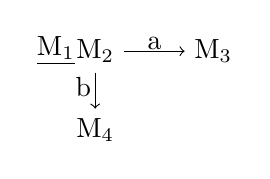
\begin{tikzpicture}
\node (M1) at (0,1) {\underline{M$_1$}};
\node (M2) at (0.5,1) {M$_2$};
\node (M3) at (2,1) {M$_3$};
\node (M4) at (0.5,0) {M$_4$};
\draw[->] (M2) -- (M3);
\draw[->] (M2) -- (M4);
\node (a) at (1.25,1.1) {a};
\node (b) at (0.35,0.55) {b};
\end{tikzpicture}
\end{center}

\item<1-> \texttt{M$_{\texttt{1--4}}$} are descriptions of Turing machines

\item<2-> Starts by executing \texttt{M$_{\texttt{1}}$}

\item<2-> When \texttt{M$_{\texttt{1}}$} halts \texttt{M$_{\texttt{2}}$} is executed starting in the machine's configuration after \texttt{M$_{\texttt{1}}$} halts
    
\item<3-> When \texttt{M$_{\texttt{2}}$} halts a decision is made

\item<3-> If an \texttt{a} is read then \texttt{M$_{\texttt{3}}$} is executed and the machine halts given that there is nothing more to execute
    
\item<3-> If a \texttt{b} is read then \texttt{M$_{\texttt{4}}$} is executed and the machine halts for the same reason
    
\item<3-> Observe that in this example a conditional jump is required to either execute \texttt{M$_{\texttt{3}}$} or \texttt{M$_{\texttt{4}}$}

\end{itemize}
\end{scriptsize}
\end{frame}

\begin{frame}[fragile]
\frametitle{Turing Machine Composition}
%\framesubtitle{HOMEWORK}
\begin{tiny}
\begin{itemize}
\item<1-> A \texttt{ctmd} is a list defined as follows:
\begin{enumerate}
 \item \tiny empty list
 \item \tiny (cons \texttt{m} \texttt{ctmd}), where \texttt{m} is either a \tm{} or a \texttt{ctmd}
 \item \tiny (cons LABEL \texttt{ctmd})
 \item \tiny (cons (list GOTO LABEL) \texttt{ctmd})
 \item \tiny (cons (BRANCH (listof (list symbol (list GOTO LABEL)))) \texttt{ctmd})
 \item \tiny (cons ((VAR symbol) \texttt{ctmd}) \texttt{ctmd})
 \item \tiny (cons variable \texttt{ctmd})
\end{enumerate}

\item<2->
\mbox{}\\
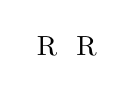
\begin{tikzpicture}
\node (R1) at (0,1) {R};
\node (R2) at (0.5,1) {R};
\end{tikzpicture}

\item<2->
\begin{alltt}
     ;; PRE:  tape = (LM w) AND i=k>0 AND w in (a b)\(\sp{*}\)
     ;; POST: tape = (LM w) AND i=k+2 AND w in (a b)\(\sp{*}\)
     (define RR (combine-tms (list R R) \quot{}(a b)))

     (check-equal? (ctm-run RR \qquot{}(,LM b a a) 1)
                   \qquot{}(F 3 (,LM b a a)))
     (check-equal? (ctm-run RR \qquot{}(,LM a a a) 2)
                   \qquot{}(F 4 (,LM a a a ,BLANK)))
     (check-equal? (ctm-run RR \qquot{}(,LM a b b a) 3)
                   \qquot{}(F 5 (,LM a b b a ,BLANK)))
     (check-equal? (ctm-run RR \qquot{}(,LM b) 1)
                   \qquot{}(F 3 (,LM b ,BLANK ,BLANK)))
\end{alltt}


\end{itemize}
\end{tiny}
\end{frame}

\begin{frame}[fragile]
\frametitle{Turing Machine Composition}
%\framesubtitle{HOMEWORK}
\begin{tiny}
\begin{itemize}
\item<1->
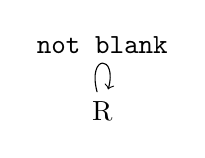
\begin{tikzpicture}
\node (R) at (0,1) {R};
\draw (R) edge[loop above] node {\tt not blank} (q2);
\end{tikzpicture}

\item<2->
\begin{alltt}
;; PRE:  tape = (LM w) AND i=k>0 AND w in (a b BLANK)\(\sp{*}\)
;; POST: tape = (LM w) AND i>k AND tape[i] = BLANK
;;       AND tape[k+1..i-1] \(\neq\) BLANK
(define FBR (combine-tms
              (list 0
                     R
                     (cons BRANCH
                           (list (list \quot{}a (list GOTO 0))
                                 (list \quot{}b (list GOTO 0))
                                 (list BLANK (list GOTO 10))))
                    10)
             (list \quot{}a \quot{}b)))

(check-equal? (ctm-run FBR \qquot{}(,LM ,BLANK) 1)
              \qquot{}(F 2 (,LM ,BLANK ,BLANK)))
(check-equal? (ctm-run FBR \qquot{}(,LM a a b b b ,BLANK a a) 2)
              \qquot{}(F 6 (,LM a a b b b ,BLANK a a)))
(check-equal? (ctm-run FBR \qquot{}(,LM ,BLANK ,BLANK b b) 3)
              \qquot{}(F 5 (,LM ,BLANK ,BLANK b b ,BLANK)))
\end{alltt}

\end{itemize}
\end{tiny}
\end{frame}

\begin{frame}[fragile]
\frametitle{Turing Machine Composition}
%\framesubtitle{HOMEWORK}
\begin{tiny}
\begin{itemize}
\item<1->
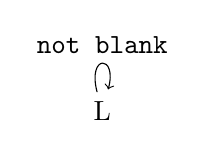
\begin{tikzpicture}
\node (R) at (0,1) {L};
\draw (R) edge[loop above] node {\tt not blank} (q2);
\end{tikzpicture}

\item<2->
\begin{alltt}
;; PRE:  tape = (LM w) AND i=k>0 AND w in (a b BLANK)\(\sp{*}\)
;; POST: tape = (LM w) AND i<k AND tape[i]=BLANK
;;       AND tape[i+1..|w|] != BLANK
(define FBL (combine-tms
              (list 0
                     L
                     (cons BRANCH
                           (list (list \quot{}a (list GOTO 0))
                                 (list \quot{}b (list GOTO 0))
                                 (list BLANK (list GOTO 1))
                                 (list LM (list GOTO 0))))
                    1)
              (list \quot{}a \quot{}b)))

(check-equal? (ctm-run FBL \qquot{}(,LM ,BLANK a a b) 4)
              \qquot{}(H 1 (,LM ,BLANK a a b)))
(check-equal?
  (ctm-run FBL \qquot{}(,LM a ,BLANK a b ,BLANK b a b b) 8)
  \qquot{}(H 5 (,LM a ,BLANK a b ,BLANK b a b b)))
\end{alltt}

\item<2-> The \texttt{BRANCH} statement in this case has a branch for processing \texttt{LM}, because \texttt{LM} may be read as it moves left

\end{itemize}
\end{tiny}
\end{frame}

\begin{frame}[fragile]
\frametitle{Turing Machine Composition}
%\framesubtitle{HOMEWORK}
\begin{scriptsize}
\begin{itemize}
\item<1-> HOMEWORK: 6, 7, 9, 10

\end{itemize}
\end{scriptsize}
\end{frame}

\begin{frame}[fragile]
\frametitle{Turing Machine Composition}
%\framesubtitle{HOMEWORK}
\begin{scriptsize}
\begin{itemize}
\item<1-> Consider the problem of adding two natural numbers

\item<1-> Must define how to represent natural numbers

\item<1-> Must define how to add two natural numbers represented using the chosen notation
    
\item<2-> Representation
\begin{alltt}
     A natural number in unary notation (nn) is either:
       1. (BLANK)
       2. (d nn)
\end{alltt}

\item<3-> Given two \texttt{nn} separated on a tape by a blank:
\begin{enumerate}
  \item \tiny Mutate the blank between the two given natural numbers to d
  \item \tiny Mutate the last i in the second argument, if any, to a blank
\end{enumerate}

\item<4-> Specification
\begin{alltt}
     ;;  PRE: tape = (LM BLANK a BLANK b) AND i = 1
     ;; POST: tape = (LM BLANK a b) AND
     ;;       i = 3                      if a = b = 0
     ;;         = numd(a) + numd(b) + 2  otherwise,
     ;;       where numd(x) = the number of d\textrm{s} in x
\end{alltt}

\end{itemize}
\end{scriptsize}
\end{frame}

\begin{frame}[fragile]
\frametitle{Turing Machine Composition}
%\framesubtitle{HOMEWORK}
\begin{tiny}
\begin{itemize}
\item<1-> Algorithm phases:
\begin{enumerate}
 \item \tiny Skip \texttt{a} and write \texttt{d} in blank after \texttt{a}
 \item \tiny Skip \texttt{b} and move head left
 \item \tiny Mutate the position under the head to a blank
 \item \tiny Move the head left and decide if the result is empty:
   \begin{enumerate}
     \item \tiny If a \texttt{d} is read move right and halt
     \item \tiny Otherwise, move to the head right twice to the blank after the blank representing 0 (the result) and halt
   \end{enumerate}
\end{enumerate}

\item<1-> These steps suggest 8 states are needed: the starting state, the final state, and 6 additional states for the steps above

\item<2-> Starting state
\begin{alltt}
     S: i = 1 and tape = (LM BLANK a BLANK b)
\end{alltt}

\item<3-> Skip \texttt{a}
\begin{alltt}
     A: i <= numd(a) + 2 and tape = (LM BLANK a BLANK b)
\end{alltt}

\item<4-> Mutate middle blank and skip \texttt{b}
\begin{alltt}
     B: i <= numd(a) + numd(b) + 3 and tape = (LM BLANK a d b)
\end{alltt}

\item<5-> Move left to mutate last \texttt{d}
\begin{alltt}
     C: i = numd(a) + numd(b) + 2 and tape = (LM BLANK a d b)
\end{alltt}

\item<6-> After mutating the last \texttt{d}
\begin{alltt}
     D: i = numd(a) + numd(b) + 2 and tape = (LM BLANK a b)
\end{alltt}

\item<7-> Move left to determine if sum is 0
\begin{alltt}
     E: i = numd(a) + numd(b) + 1 and tape = (LM BLANK a b)
\end{alltt}

\item<8-> Place head to meet postcondition
\begin{alltt}
     G: i = numd(a) + numd(b) + 2 and tape = (LM BLANK)
     F: i = 3                      if a = b = 0
          = numd(a) + numd(b) + 2  otherwise
        and tape = (LM BLANK a b)
\end{alltt}

\end{itemize}
\end{tiny}
\end{frame}

\begin{frame}[fragile]
\frametitle{Turing Machine Composition}
%\framesubtitle{HOMEWORK}
\begin{tiny}
\begin{itemize}
\item<1->
\begin{alltt}
     ;;  PRE: tape = (LM BLANK a BLANK b) AND i = 1
     ;; POST: tape = (LM BLANK a b) AND
     ;;       i = 3                     if a = b = 0
     ;;         = numd(a) + numd(b) + 2 otherwise,
     ;;       where numd(x) = the number of d\textrm{s} in x
     (define ADD (make-tm \quot{}(S A B C D E F G)
                          \quot{}(d)
\end{alltt}

\item<3->
\begin{alltt}
                          \qquot{}(((S ,BLANK) (A ,RIGHT))
\end{alltt}

\item<4->
\begin{alltt}
                            ((A d) (A ,RIGHT))
                            ((A ,BLANK) (B d))
\end{alltt}

\item<5->
\begin{alltt}
                            ((B d) (B ,RIGHT))
                            ((B ,BLANK) (C ,LEFT))
\end{alltt}

\item<6->
\begin{alltt}
                            ((C d) (D ,BLANK))
\end{alltt}

\item<7->
\begin{alltt}
                            ((D ,BLANK) (E ,LEFT))
\end{alltt}

\item<8->
\begin{alltt}
                            ((E d) (F ,RIGHT))
                            ((E ,BLANK) (G ,RIGHT))
\end{alltt}

\item<9->
\begin{alltt}
                            ((G ,BLANK) (F ,RIGHT)))
\end{alltt}

\item<1->
\begin{alltt}
                          \quot{}S
                          \quot{}(F)))
\end{alltt}

\item<2->
\begin{alltt}
     (check-equal?
      (last (sm-showtransitions ADD \qquot{}(,LM ,BLANK ,BLANK ,BLANK) 1))
      \qquot{}(F 3 (,LM ,BLANK ,BLANK ,BLANK)))
     (check-equal?
      (last (sm-showtransitions ADD \qquot{}(,LM ,BLANK ,BLANK d d d ,BLANK) 1))
      \qquot{}(F 5 (,LM ,BLANK d d d ,BLANK ,BLANK)))
     (check-equal?
      (last (sm-showtransitions ADD \qquot{}(,LM ,BLANK d d ,BLANK ,BLANK) 1))
      \qquot{}(F 4 (,LM ,BLANK d d ,BLANK ,BLANK)))
     (check-equal?
      (last (sm-showtransitions ADD \qquot{}(,LM ,BLANK d d ,BLANK d d d) 1))
      \qquot{}(F 7 (,LM ,BLANK d d d d d ,BLANK ,BLANK)))
\end{alltt}

\end{itemize}
\end{tiny}
\end{frame}

\begin{frame}[fragile]
\frametitle{Turing Machine Composition}
%\framesubtitle{HOMEWORK}
\begin{scriptsize}
\begin{itemize}
\item<1-> To establish correctness we use Hoare Logic (if you have read \emph{Animated Program Design} then you are familiar with it)
    
\item<2-> To establish the correctness of mutation-based computations use a triple for each rule:
\begin{alltt}
     ((X i) (Y a))
\end{alltt}

\item<2-> The corresponding triple is:
\begin{alltt}
     <Assertion about X's role>
     ((X i) (Y a))
     <Assertion about Y's role>
\end{alltt}

\item<2-> A triple is valid if assuming the precondition and the execution of the transition implies the postcondition
    
\end{itemize}
\end{scriptsize}
\end{frame}

\begin{frame}[fragile]
\frametitle{Turing Machine Composition}
%\framesubtitle{HOMEWORK}
\begin{tiny}

\begin{theorem}
ADD computes the addition of two natural numbers and leaves the head on the first blank after the result.
\end{theorem}

\begin{proof}
\begin{itemize}
\item<1-> Proof by induction on the number of transitions performed by a computation

\item<2-> \underline{Base case (n = 0)}: The machine starts in S and, by assumption, the precondition is true. Therefore, the role of S is satisfied.

\item<2-> \underline{Inductive Step}:\\
\noindent  Assume: State roles satisfied for n = k\\
\noindent Show: that State roles satisfied for n = k + 1

\item<3->
\begin{alltt}
     \emph{i = 1 and tape = (LM BLANK a BLANK b)}
     ((S ,BLANK) (A ,RIGHT))
     \emph{i <= numd(a) + 2 and tape = (LM BLANK a BLANK b)}
\end{alltt}

\item<4->
\begin{alltt}
     \emph{i <= numd(a) + 2 and tape = (LM BLANK a BLANK b)}
     ((A d) (A ,RIGHT))
     \emph{i <= numd(a) + 2 and tape = (LM BLANK a BLANK b)}
\end{alltt}

\item<5->
\begin{alltt}
     \emph{i <= numd(a) + 2 and tape = (LM BLANK a BLANK b)}
     ((A ,BLANK) (B d))
     \emph{i <= numd(a) + numd(b) + 3 and tape = (LM BLANK a d b)}
\end{alltt}

\item<6->
\begin{alltt}
     \emph{i <= numd(a) + numd(b) + 3 and tape = (LM BLANK a d b)}
     ((B d) (B ,RIGHT))
     \emph{i <= numd(a) + numd(b) + 3 and tape = (LM BLANK a d b)}
\end{alltt}

\item<7->
\begin{alltt}
     \emph{i <= numd(a) + numd(b) + 3 and tape = (LM BLANK a d b)}
     ((B ,BLANK) (C ,LEFT))
     \emph{i = numd(a) + numd(b) + 2 and tape = (LM BLANK a d b)}
\end{alltt}

\end{itemize}
\end{proof}

\end{tiny}
\end{frame}

\begin{frame}[fragile]
\frametitle{Turing Machine Composition}
%\framesubtitle{HOMEWORK}
\begin{tiny}

\begin{theorem}
ADD computes the addition of two natural numbers and leaves the head on the first blank after the result.
\end{theorem}

\begin{proof}
\begin{itemize}
\item<1-> \underline{Inductive Step}:\\
\noindent  Assume: State roles satisfied for n = k\\
\noindent Show: that State roles satisfied for n = k + 1\\
\vdotss{}

\item<1->
\begin{alltt}
     \emph{i = numd(a) + numd(b) + 2 and tape = (LM BLANK a d b)}
     ((C d) (D ,BLANK))
     \emph{i = numd(a) + numd(b) + 2 and tape = (LM BLANK a b)}
\end{alltt}

\item<2->
\begin{alltt}
     \emph{i = numd(a) + numd(b) + 2 and tape = (LM BLANK a b)}
     ((D ,BLANK) (E ,LEFT))
     \emph{i = numd(a) + numd(b) + 1 and tape = (LM BLANK a b)}
\end{alltt}

\item<3->
\begin{alltt}
     \emph{i = numd(a) + numd(b) + 1 and tape = (LM BLANK a b)}
     ((E d) (F ,RIGHT))
     \emph{i = 3                     if a = b = 0
       = numd(a) + numd(b) + 2 otherwise
     \(\wedge\) tape = (LM BLANK a b)}
\end{alltt}

\item<4->
\begin{alltt}
     \emph{i = numd(a) + numd(b) + 1 and tape = (LM BLANK a b)}
     ((E ,BLANK) (G ,RIGHT))
     \emph{i = numd(a) + numd(b) + 2 and tape = (LM BLANK BLANK)}
\end{alltt}

\item<5->
\begin{alltt}
     \emph{i = numd(a) + numd(b) + 2 and tape = (LM BLANK BLANK)}
     ((G ,BLANK) (F ,RIGHT))
     \emph{i = 3                     if a = b = 0
       = numd(a) + numd(b) + 2 otherwise
     \(\wedge\) tape = (LM BLANK a b)}
\end{alltt}

\end{itemize}
\end{proof}

\end{tiny}
\end{frame}

\begin{frame}[fragile]
\frametitle{Turing Machine Composition}
%\framesubtitle{HOMEWORK}
\begin{tiny}
\begin{itemize}
\item<1-> \tiny Copy machine
\begin{alltt}
;PRE: tape=(LM BLANK w BLANK) && i=|w|+2
;POST: tape=(LM BLANK w BLANK w BLANK) && i=2|w|+3
\end{alltt}

\item<2-> \tiny Move to the first blank to the left and then move right

\item<3-> \tiny Branch on the element read
  \begin{itemize}
    \item<3-> \tiny the next element to copy
    \item<3-> \tiny the blank after \texttt{w}
  \end{itemize}

\item<4-> \tiny If a blank is read then the tape contains two copies of \texttt{w} separated by a blank and the machine must place the head correctly to satisfy the postcondition
    
    \begin{itemize}
      \item<4-> \tiny The head must be moved to the first blank to the right and then moved left
      \item<4-> \tiny A second branch is needed to determine if \texttt{w} is empty
      \item<4-> \tiny If a blank is read then \texttt{w} is empty and the head is moved twice to the right to satisfy the postcondition
      
      \item<4-> \tiny Otherwise, the head is moved once to the right to satisfy the postcondition
    \end{itemize}

\item<5-> \tiny If an alphabet element is read at the first branching point then the machine must make a copy of the element and loop to repeat the process for any remaining elements to copy
    \begin{itemize}
      \item<5-> \tiny The read value is captured in a variable and then overwritten with a blank as a placeholder to remember the read element's position
          
      \item<5-> \tiny The machine moves to the second blank to the right and mutates this blank to be the value of the variable
          
      \item<5-> \tiny It then moves to the second blank to the left and restores the value previously overwritten with a blank
          
      \item<5-> \tiny The machine loops to move right and reach the first branching point again
    \end{itemize}

\end{itemize}
\end{tiny}
\end{frame}

\begin{frame}[fragile]
\frametitle{Turing Machine Composition}
%\framesubtitle{HOMEWORK}
\begin{scriptsize}
\begin{itemize}
\item<1->
\includegraphics[scale=0.20]{COPYv2.png}

\end{itemize}
\end{scriptsize}
\end{frame}

\begin{frame}[fragile]
\frametitle{Turing Machine Composition}
%\framesubtitle{HOMEWORK}
\begin{tiny}
\begin{itemize}
\item<1-> Correctness
\begin{alltt}
 \emph{(LM BLANK a\(\sb{1}\)\dotss{}a\(\sb{n}\) \underline{BLANK}) \(\vee\) (LM BLANK BLANK \underline{BLANK})}
 FBL
 \emph{(LM \underline{BLANK} a\(\sb{1}\)\dotss{}a\(\sb{n}\) BLANK) \(\vee\) (LM BLANK \underline{BLANK} BLANK)}
\end{alltt}

\item<2->
\begin{alltt}
\emph{(LM \underline{BLANK} a\(\sb{1}\)\dotss{}a\(\sb{n}\) BLANK) \(\vee\) (LM BLANK \underline{BLANK} BLANK)}
\(\vee\) (LM BLANK a\(\sb{1}\)\dotss{}\underline{a\(\sb{i}\)}\dotss{}a\(\sb{n}\) BLANK a\(\sb{1}\)\dotss{}a\(\sb{i-1}\))
R
\emph{(LM BLANK a\(\sb{1}\)\dotss{}\underline{a\(\sb{j}\)}\dotss{}a\(\sb{n}\) BLANK)
\(\vee\) (LM BLANK BLANK \underline{BLANK})}
\end{alltt}

\item<3->
\begin{alltt}
\emph{(LM BLANK a\(\sb{1}\)\dotss{}\underline{a\(\sb{i}\)}\dotss{}a\(\sb{n}\) BLANK a\(\sb{1}\)\dotss{}a\(\sb{i-1}\))}
(list VAR \quot{}k)
\emph{(LM BLANK a\(\sb{1}\)\dotss{}\underline{a\(\sb{i}\)}\dotss{}a\(\sb{n}\) BLANK a\(\sb{1}\)\dotss{}a\(\sb{i-1}\)) \(\wedge\) k=a\(\sb{i}\)}
\end{alltt}

\item<4->
\begin{alltt}
FBR
\emph{(LM BLANK a\(\sb{1}\)\dotss{}a\(\sb{i}\)\dotss{}a\(\sb{n}\) \underline{BLANK} a\(\sb{1}\)\dotss{}a\(\sb{i-1}\)) \(\wedge\) k=a\(\sb{i}\)}
\end{alltt}

\item<5->
\begin{alltt}
FBR
\emph{(LM BLANK a\(\sb{1}\)\dotss{}BLANK\dotss{}a\(\sb{n}\) BLANK a\(\sb{1}\)\dotss{}a\(\sb{i-1}\) \underline{BLANK}) \(\wedge\) k=a\(\sb{i}\)}
\end{alltt}

\item<6->
\begin{alltt}
\quot{}k
\emph{(LM BLANK a\(\sb{1}\)\dotss{}BLANK\dotss{}a\(\sb{n}\) BLANK a\(\sb{1}\)\dotss{}a\(\sb{i-1}\) \underline{a\(\sb{i}\)}) \(\wedge\) k=a\(\sb{i}\)}
\end{alltt}

\item<7>
\begin{alltt}
FBL
\emph{(LM BLANK a\(\sb{1}\)\dotss{}BLANK\dotss{}a\(\sb{n}\) \underline{BLANK} a\(\sb{1}\)\dotss{}a\(\sb{i-1}\) a\(\sb{i}\)) && k=a\(\sb{i}\)}
\end{alltt}

\end{itemize}
\end{tiny}
\end{frame}

\begin{frame}[fragile]
\frametitle{Turing Machine Composition}
%\framesubtitle{HOMEWORK}
\begin{tiny}
\begin{itemize}
\item<1->
\begin{alltt}
FBL
\emph{(LM BLANK a\(\sb{1}\)\dotss{}BLANK\dotss{}a\(\sb{n}\) \underline{BLANK} a\(\sb{1}\)\dotss{}a\(\sb{i-1}\) a\(\sb{i}\)) && k=a\(\sb{i}\)}
\end{alltt}

\item<1->
\begin{alltt}
FBL
\emph{(LM BLANK a\(\sb{1}\)\dotss{}\underline{BLANK}\dotss{}a\(\sb{n}\) BLANK a\(\sb{1}\)\dotss{}a\(\sb{i-1}\) a\(\sb{i}\)) && k=a\(\sb{i}\)}
\end{alltt}

\item<2->
\begin{alltt}
\quot{}k
\emph{(LM BLANK a\(\sb{1}\)\dotss{}\underline{a\(\sb{i}\)}\dotss{}a\(\sb{n}\) BLANK a\(\sb{1}\)\dotss{}a\(\sb{i-1}\) a\(\sb{i}\))}
\end{alltt}

\item<2-> Precondition for label 0, starting with \texttt{R}, is met

\item<3-> Label 2 is only reached by reading a blank in the branch of the machine at label 0
\begin{alltt}
\emph{(LM BLANK a\(\sb{1}\)\dotss{}a\(\sb{n}\) \underline{BLANK} a\(\sb{1}\)\dotss{}a\(\sb{n}\)) \(\vee\)
(LM BLANK BLANK \underline{BLANK})}
FBR
\emph{(LM BLANK a\(\sb{1}\)\dotss{}a\(\sb{n}\) BLANK a\(\sb{1}\)\dotss{}a\(\sb{n}\) \underline{BLANK}) \(\vee\)
(LM BLANK BLANK BLANK \underline{BLANK})}
\end{alltt}

\item<4->
\begin{alltt}
L
\emph{(LM BLANK a\(\sb{1}\)\dotss{}a\(\sb{n}\) BLANK a\(\sb{1}\)\dotss{}\underline{a\(\sb{n}\)} BLANK) \(\vee\)
(LM BLANK BLANK \underline{BLANK} BLANK)}
\end{alltt}

\item<5-> Label 3 is only reached if a blank is read at the end of the machine, \texttt{L}, at label 2: input word is empty and the head is over it:
\begin{alltt}
\emph{(LM BLANK BLANK \underline{BLANK} BLANK)}
RR
\emph{(LM BLANK BLANK BLANK BLANK \underline{BLANK})}
\end{alltt}

\item<6-> Label 4 is only reached if the head is over the last element of the nonempty input word's copy at the end of label 2:
\begin{alltt}
\emph{(LM BLANK a\(\sb{1}\)\dotss{}a\(\sb{n}\) BLANK a\(\sb{1}\)\dotss{}\underline{a\(\sb{n}\)} BLANK)}
R
\emph{(LM BLANK a\(\sb{1}\)\dotss{}a\(\sb{n}\) BLANK a\(\sb{1}\)\dotss{}a\(\sb{n}\) \underline{BLANK})}
\end{alltt}

\end{itemize}
\end{tiny}
\end{frame}

\begin{frame}[fragile]
\frametitle{Turing Machine Composition}
%\framesubtitle{HOMEWORK}
\begin{scriptsize}
\begin{itemize}
\item<1-> HOMEWORK: 12--15

\end{itemize}
\end{scriptsize}
\end{frame}


\section{Turing Machine Extensions}

\begin{frame}[fragile]
\frametitle{Turing Machine Extensions}
%\framesubtitle{HOMEWORK}
\begin{scriptsize}
\begin{itemize}
\item<1-> Turing machines are powerful enough to recognize languages that are not context-free and to compute arbitrary functions

\item<1-> Hard to program! 

\item<2-> An unanswered question in Computer Science is whether or not there are (undiscovered) machines that are more powerful

\item<2-> Many attempts to strengthen Turing machines akin to strengthening \ndfa{}'s with a stack 

\item<2-> None have been successful

\item<2-> Many computer scientists today believe that the Turing machine is the most powerful computational device 

\item<3-> Why study new automata models that are not more powerful than the Turing machine? 

\item<4-> Make problem solving easier

\end{itemize}
\end{scriptsize}
\end{frame}

\begin{frame}[fragile]
\frametitle{Turing Machine Extensions}
%\framesubtitle{HOMEWORK}
\begin{scriptsize}
\begin{itemize}
\item<1->
\begin{figure}[t!]
\begin{center}
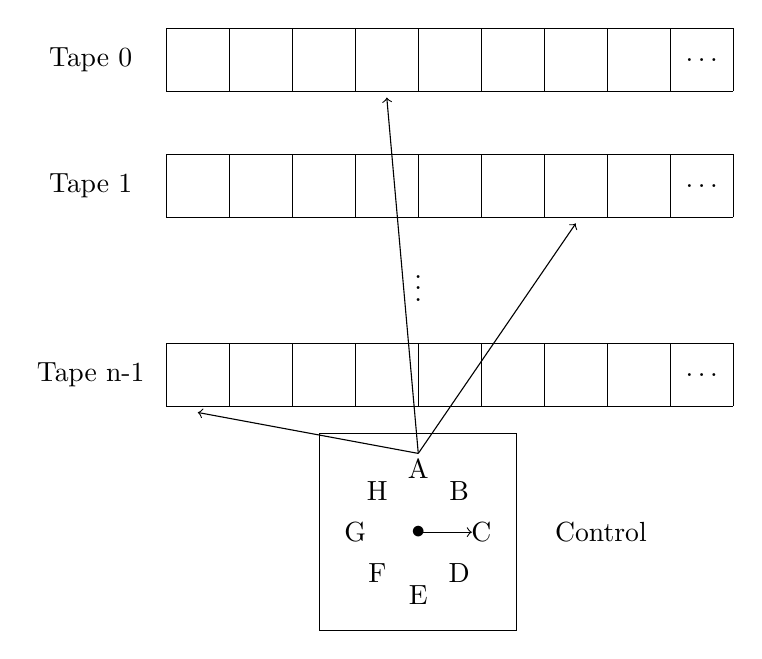
\begin{tikzpicture}[scale=0.8]
\draw (5,10) grid (6,11); %input tape n-1
\draw (6,10) grid (7,11);
\draw (7,10) grid (8,11);
\draw (8,10) grid (9,11);
\draw (9,10) grid (10,11);
\draw (10,10) grid (11,11);
\draw (11,10) grid (12,11);
\draw (12,10) grid (13,11);
\draw (13,10) grid (14,11);
\draw (5,13) grid (6,14); %input tape 1
\draw (6,13) grid (7,14);
\draw (7,13) grid (8,14);
\draw (8,13) grid (9,14);
\draw (9,13) grid (10,14);
\draw (10,13) grid (11,14);
\draw (11,13) grid (12,14);
\draw (12,13) grid (13,14);
\draw (13,13) grid (14,14);
\draw (5,15) grid (6,16); %input tape 0
\draw (6,15) grid (7,16);
\draw (7,15) grid (8,16);
\draw (8,15) grid (9,16);
\draw (9,15) grid (10,16);
\draw (10,15) grid (11,16);
\draw (11,15) grid (12,16);
\draw (12,15) grid (13,16);
\draw (13,15) grid (14,16);
%\draw (5.5,10.5) node {a}; %tape contents
%\draw (6.5,10.5) node {a};
%\draw (7.5,10.5) node {a};
%\draw (8.5,10.5) node {a};
%\draw (9.5,10.5) node {a};
%\draw (10.5,10.5) node {b};
%\draw (11.5,10.35) node {--};
%\draw (12.5,10.35) node {--};
\draw (9,12) node {\vdotss};
\draw (13.5,10.5) node {\dotss};
\draw (13.5,13.5) node {\dotss};
\draw (13.5,15.5) node {\dotss};
\draw (9,8) node[minimum size=2.5cm,draw] {$\bullet$}; %control
\draw (9,9) node {A};
\draw (9.65,8.65) node {B};
\draw (10,8) node {C};
\draw (9.65,7.35) node {D};
\draw (9,7) node {E};
\draw (8.35,7.35) node {F};
\draw (8,8) node {G};
\draw (8.35,8.65) node {H};
\draw[->] (9,8) -- (9.85,8); %control arrow
\draw[->] (9,9.25) -- (5.5,9.9); %head arrow
\draw[->] (9,9.25) -- (11.5,12.9); %head arrow
\draw[->] (9,9.25) -- (8.5,14.9); %head arrow
\draw (3.8,10.5) node {Tape n-1};
\draw (3.8,13.5) node {Tape 1};
\draw (3.8,15.5) node {Tape 0};
\draw (11.9,8) node {Control};
%\draw (9.85,9.58) node {Head};
\end{tikzpicture}
\end{center}
\end{figure}

\end{itemize}
\end{scriptsize}
\end{frame}

\begin{frame}[fragile]
\frametitle{Turing Machine Extensions}
%\framesubtitle{HOMEWORK}
\begin{scriptsize}
\begin{itemize}
\item<1-> A multitape Turing machine (\mttm) with \texttt{n}-tapes is an instance of:
\begin{alltt}
     (make-mttm K \sig S F \delt n [Y])
\end{alltt}

\item<2-> \underline{\texttt{K}}: A list of states. Each state is denoted by a symbol that represents a capital letter in the Roman alphabet
\item<2-> \underline{\texttt{\sig}}: A list of symbols or digits. Each symbol represents a lowercase letter in the Roman alphabet.
\item<2-> \underline{\texttt{S}}: The starting state. It must be a member of \texttt{K}.
\item<2-> \underline{\texttt{F}}: A list of final states. Each state must be a member of \texttt{K}.
\item<3-> \underline{\texttt{\delt}}:] A list of transition rules defining a transition relation. Each transition rule has the following type:
      \begin{alltt}
         (list (list state (list symbol\(\sp{\texttt{n}}\)))
               (list state (list action\(\sp{\texttt{n}}\))))
      \end{alltt}
\item<4-> \underline{\texttt{n}}: A natural number greater than or equal to 1 representing the number of tapes.
\item<4-> \underline{\texttt{Y}}: An optional argument representing the accepting state for a language recognizer

\end{itemize}
\end{scriptsize}
\end{frame}

\begin{frame}[fragile]
\frametitle{Turing Machine Extensions}
%\framesubtitle{HOMEWORK}
\begin{scriptsize}
\begin{itemize}
\item<1-> A configuration
\begin{alltt}
     \qquot{}(D
       (9 (,LM ,BLANK a a b b c c d d ,BLANK))
       (3 (,BLANK b b ,BLANK))
       (3 (,BLANK c c ,BLANK))
       (3 (,BLANK d d ,BLANK)))
\end{alltt}

\item<1-> The machine is in state \texttt{D}. On tape 0 the head is on position 9 and on tapes 1--3 the heads are on position 3

\item<2-> A transition made by the machine is denoted using \step

\item<2-> \texttt{C$_i$} \step \ \texttt{C$_{j}$} is valid for \texttt{M} if and only if \texttt{M} can move from \texttt{C$_i$} to \texttt{C$_{j}$} using a single transition
    
\item<3-> Zero or more moves by \texttt{M} is denoted using \steps

\item<3-> \texttt{C$_{i}$} \steps{} \texttt{C$_{j}$} is valid for \texttt{M} if and only if \texttt{M} can move from \texttt{C$_i$} to \texttt{C$_{j}$} using zero or more transitions
    
\item<4-> An \mttm{} language recognizer accepts a word, \texttt{w}, if there is a computation that reaches its accepting state

\end{itemize}
\end{scriptsize}
\end{frame}


\begin{frame}[fragile]
\frametitle{Turing Machine Extensions}
%\framesubtitle{HOMEWORK}
\begin{scriptsize}
\begin{itemize}
\item<1-> L = \{w $|$ w has equal number of \texttt{a}s, \texttt{b}s, and \texttt{c}s\texttt{\}}

\item<2-> Step 1

\item<2-> The machine is named \texttt{EQABC} and \sig{} = \{\texttt{a} \texttt{b} \texttt{c}\}.

\item<3-> Let \texttt{t0h} be the position of the head on tape 0

\item<3-> The precondition for \texttt{EQABC} is:
\begin{alltt}
  ;; PRE: (LM BLANK w) AND t0h = 1 AND tapes 1-3 are empty AND
  ;;      t1h-t3h = 0
\end{alltt}
\end{itemize}
\end{scriptsize}
\end{frame}



\begin{frame}[fragile]
\frametitle{Turing Machine Extensions}
%\framesubtitle{HOMEWORK}
\begin{scriptsize}
\begin{itemize}
\item<1-> Step 2
\begin{alltt}
  (check-equal? (sm-apply EQABC \qquot{}(,LM ,BLANK a a b b a c c) 1)
                \quot{}reject)
  (check-equal? (sm-apply EQABC \qquot{}(,LM ,BLANK a a a) 1)
                \quot{}reject)
  (check-equal? (sm-apply EQABC \qquot{}(,LM ,BLANK c c a b b) 1)
                \quot{}reject)
  (check-equal? (sm-apply EQABC \qquot{}(,LM ,BLANK) 1) \quot{}accept)
  (check-equal? (sm-apply EQABC \qquot{}(,LM ,BLANK a c c b a b) 1)
                \quot{}accept)
  (check-equal?
   (sm-apply EQABC
             \qquot{}(,LM ,BLANK c c c a b b a a c b a b b c a) 1)
   \quot{}accept)
\end{alltt}

\end{itemize}
\end{scriptsize}
\end{frame}

\begin{frame}[fragile]
\frametitle{Turing Machine Extensions}
%\framesubtitle{HOMEWORK}
\begin{scriptsize}
\begin{itemize}
\item<1-> Step 3: Conditions and States

\item<2-> Design Idea

\item<2-> A 4-tape machine

\item<2-> \texttt{T0}, contains the input word and is never mutated

\item<2-> \texttt{T1}, \texttt{T2}, and \texttt{T3}, are used to store copies, respectively, of the \texttt{a}s, \texttt{b}s, and \texttt{c}s 

\item<3-> The machine operates in two phases

\item<3-> First phase, the input word elements are copied to the auxiliary tapes

\item<4-> Second phase, the auxiliary tapes are simultaneously traversed to determine if for each \texttt{a} there is a matching \texttt{b} and a matching \texttt{c}
    
\item<5-> If a blank is read on all three auxiliary tapes then the machine moves to accept

\item<5-> If a blank is read on any tape, but not all tapes, then the machines moves to reject

\item<5-> Otherwise, the machine moves the heads on each auxiliary tape to the left. 

\end{itemize}
\end{scriptsize}
\end{frame}

\begin{frame}[fragile]
\frametitle{Turing Machine Extensions}
%\framesubtitle{HOMEWORK}
\begin{scriptsize}
\begin{itemize}
\item<1-> In more detail \dotss{}

\item<1-> The machine starts by moving all 4 heads to the right: \texttt{T0} over the next element, if any, to copy and auxiliary heads on the next position to copy to
    
\item<2-> Phase 1 that operates as follows:
\begin{enumerate}
  \item If a blank is read on \texttt{T0} then move the heads on the auxiliary tapes to the left and goto to Phase 2.
  \item Otherwise, copy the read symbol on \texttt{T0} to the respective auxiliary tape.
  \item Move the head of the auxiliary tape copied to and move \texttt{T0}'s head to the right and goto Phase 1's first step.
\end{enumerate}

\item<3-> Phase 2 operates as follows:
\begin{enumerate}
  \item If a blank is read on all tapes move to accept
  \item If an \texttt{a} is read on \texttt{T1}, a \texttt{b} is read on \texttt{T2}, and a \texttt{c} is read on \texttt{T3} then move the heads on all auxiliary tapes to the left and goto Phase 2's second step.
  \item Otherwise, halt and reject.
\end{enumerate}

\end{itemize}
\end{scriptsize}
\end{frame}

\begin{frame}[fragile]
\frametitle{Turing Machine Extensions}
%\framesubtitle{HOMEWORK}
\begin{tiny}
\begin{itemize}
\item<1-> 
\begin{alltt}
S: 
   tape 0 = (LM BLANK w) AND t0h = 1
   tape 1-3 = (BLANK) AND t1h = t2h = t3h = 0
   starting state
\end{alltt}

\item<2->
\begin{alltt}
C:
   tape 0 = (LM BLANK w)
   t0h >= 2
\end{alltt}

\item<3->
\begin{alltt}  
   tape 1 = (BLANK a\(\sp{*}\) BLANK)
   tape 1 num a = if (eq? tape1[t1h] BLANK)
                     num a in tape0[2..t0h-1]
                     num a in tape0[2..t0h]
   t1h = if (eq? tape1[t1h] BLANK)
            num a in tape1[2..t0h-1] + 1
            num a in tape1[2..t0h] + 1
\end{alltt}

\item<4->
\begin{alltt}  
   tape 2 = (BLANK b\(\sp{*}\) BLANK)
   tape 2 num b = if (eq? tape2[t2h] BLANK)
                     num b in tape0[2..t0h-1]
                     num b in tape0[2..t0h]
   t2h = if (eq? tape2[t2h] BLANK)
            num b in tape2[2..t0h-1] + 1
            num b in tape2[2..t0h] + 1
\end{alltt}

\item<5->
\begin{alltt}  
   tape 3 = (BLANK c\(\sp{*}\) BLANK)
   tape 3 num c = if (eq? tape3[t3h] BLANK)
                     num c in tape0[2..t0h-1]
                     num c in tape0[2..t0h]
   t3h = if (eq? tape3[t3h] BLANK)
            num c in tape3[2..t0h-1] + 1
            num c in tape3[2..t0h] + 1
\end{alltt}

\end{itemize}
\end{tiny}
\end{frame}



\begin{frame}[fragile]
\frametitle{Turing Machine Extensions}
%\framesubtitle{HOMEWORK}
\begin{scriptsize}
\begin{itemize}
\item<1->
\begin{alltt}
G: 
   tape 0 = (LM BLANK w)
   t1 = (BLANK a*)
   t2 = (BLANK b*)
   t3 = (BLANK c*)
   num a in t0 = num a in t1
   num b in t0 = num b in t2
   num c in t0 = num c in t3
   (= |as matched| |bs matched| |cs matched|)
\end{alltt}

\item<2->
\begin{alltt}
Y: 
   num a in t0 = num a in t1
   num b in t0 = num b in t2
   num c in t0 = num c in t3
   num a in t1 = num b in t2 = num c in t3
   final and accepting state
\end{alltt}

\end{itemize}
\end{scriptsize}
\end{frame}

\begin{frame}[fragile]
\frametitle{Turing Machine Extensions}
%\framesubtitle{HOMEWORK}
\begin{scriptsize}
\begin{itemize}
\item<1-> Step 4: Transition Relation

\item<1->
\begin{alltt}
     (list (list \quot{}S (list BLANK BLANK BLANK BLANK))
           (list \quot{}C (list RIGHT RIGHT RIGHT RIGHT)))
\end{alltt}

\item<2->
\begin{alltt}
;; read a on t0, copy to t1 and then move R on t0 and t1
(list (list \quot{}C (list \quot{}a BLANK BLANK BLANK))
      (list \quot{}C (list \quot{}a \quot{}a BLANK BLANK)))
(list (list \quot{}C (list \quot{}a \quot{}a BLANK BLANK))
      (list \quot{}C (list RIGHT RIGHT BLANK BLANK)))
\end{alltt}
      
\item<3->
\begin{alltt}
(list (list \quot{}C (list \quot{}b BLANK BLANK BLANK))
      (list \quot{}C (list \quot{}b BLANK \quot{}b BLANK)))
(list (list \quot{}C (list \quot{}b BLANK \quot{}b BLANK))
      (list \quot{}C (list RIGHT BLANK RIGHT BLANK)))
\end{alltt}
      
\item<4->
\begin{alltt}
(list (list \quot{}C (list \quot{}c BLANK BLANK BLANK))
      (list \quot{}C (list \quot{}c BLANK BLANK \quot{}c)))
(list (list \quot{}C (list \quot{}c BLANK BLANK \quot{}c))
      (list \quot{}C (list RIGHT BLANK BLANK RIGHT)))
\end{alltt}

\item<5->
\begin{alltt}
(list (list \quot{}C (list BLANK BLANK BLANK BLANK))
      (list \quot{}G (list BLANK LEFT LEFT LEFT)))
\end{alltt}

\end{itemize}
\end{scriptsize}
\end{frame}

\begin{frame}[fragile]
\frametitle{Turing Machine Extensions}
%\framesubtitle{HOMEWORK}
\begin{scriptsize}
\begin{itemize}
\item<1-> 
\begin{alltt}
(list (list \quot{}G (list BLANK \quot{}a \quot{}b \quot{}c))
      (list \quot{}G (list BLANK LEFT LEFT LEFT)))
\end{alltt}

\item<2->
\begin{alltt}
(list (list \quot{}G (list BLANK BLANK BLANK BLANK))
      (list \quot{}Y (list BLANK BLANK BLANK BLANK)))
\end{alltt}

\end{itemize}
\end{scriptsize}
\end{frame}

\begin{frame}[fragile]
\frametitle{Turing Machine Extensions}
%\framesubtitle{HOMEWORK}
\begin{tiny}
\begin{itemize}
\item<1-> Steps 5 \& 6: Implement and test
\begin{alltt}
     #lang fsm
     ;; L = {w | w has an equal number of a, b, and c}  PRE: t0 = (LM BLANK w) AND i = 1
     (define EQABC (make-mttm \quot{}(S C G Y)
                              \quot{}(a b c)
                              \quot{}S
                              \quot{}(Y)
                              (list 
                               (list (list \quot{}S (list BLANK BLANK BLANK BLANK))
                                     (list \quot{}C (list RIGHT RIGHT RIGHT RIGHT)))
                               (list (list \quot{}C (list \quot{}a BLANK BLANK BLANK))
                                     (list \quot{}C (list \quot{}a \quot{}a BLANK BLANK)))
                               (list (list \quot{}C (list \quot{}a \quot{}a BLANK BLANK))
                                     (list \quot{}C (list RIGHT RIGHT BLANK BLANK)))
                               (list (list \quot{}C (list \quot{}b BLANK BLANK BLANK))
                                     (list \quot{}C (list \quot{}b BLANK \quot{}b BLANK)))
                               (list (list \quot{}C (list \quot{}b BLANK \quot{}b BLANK))
                                     (list \quot{}C (list RIGHT BLANK RIGHT BLANK)))
                               (list (list \quot{}C (list \quot{}c BLANK BLANK BLANK))
                                     (list \quot{}C (list \quot{}c BLANK BLANK \quot{}c)))
                               (list (list \quot{}C (list \quot{}c BLANK BLANK \quot{}c))
                                     (list \quot{}C (list RIGHT BLANK BLANK RIGHT)))
                               (list (list \quot{}C (list BLANK BLANK BLANK BLANK))
                                     (list \quot{}G (list BLANK LEFT LEFT LEFT)))
                               (list (list \quot{}G (list BLANK BLANK BLANK BLANK))
                                     (list \quot{}Y (list BLANK BLANK BLANK BLANK)))
                               (list (list \quot{}G (list BLANK \quot{}a \quot{}b \quot{}c))
                                     (list \quot{}G (list BLANK LEFT LEFT LEFT))))
                              4
                              \quot{}Y))
     (check-equal? (sm-apply EQABC \qquot{}(,LM ,BLANK a a b b a c c) 1) \quot{}reject)
     (check-equal? (sm-apply EQABC \qquot{}(,LM ,BLANK a a a) 1) \quot{}reject)
     (check-equal? (sm-apply EQABC \qquot{}(,LM ,BLANK c c a b b) 1) \quot{}reject)
     (check-equal? (sm-apply EQABC \qquot{}(,LM ,BLANK) 1) \quot{}accept)
     (check-equal? (sm-apply EQABC \qquot{}(,LM ,BLANK a b c) 1) \quot{}accept)
     (check-equal? (sm-apply EQABC \qquot{}(,LM ,BLANK a c c b a b) 1) \quot{}accept)
     (check-equal? (sm-apply EQABC \qquot{}(,LM ,BLANK c c c a b b a a c b a b b c a) 1) \quot{}accept)
\end{alltt}
\end{itemize}
\end{tiny}
\end{frame}

\begin{frame}[fragile]
\frametitle{Turing Machine Extensions}
%\framesubtitle{HOMEWORK}
\begin{scriptsize}
\begin{itemize}
\item<1-> Step 7: Invariant Predicates

\item<1-> For \mttm{}s, an invariant predicate takes a (listof tape-config)

\item<1-> Tape 0--Tape N-1

\item<2-> A tape configuration: (tape-head tape-value)

\end{itemize}
\end{scriptsize}
\end{frame}

\begin{frame}[fragile]
\frametitle{Turing Machine Extensions}
%\framesubtitle{HOMEWORK}
\begin{tiny}
\begin{itemize}
\item<1-> Step 7: Invariant Predicates
\begin{alltt}
S: tape 0 = (LM BLANK w) AND t0h = 1
   tape 1-3 = (BLANK) AND t1h = t2h = t3h = 0
   starting state
\end{alltt}

\item<2->
\begin{alltt}
;; (listof tape-config) \arrow{} Boolean
;; Purpose: Determine if S's conditions are met
(define (S-INV tape-configs)
  (let* [(t0c (first tape-configs))
         (t1c (second tape-configs))
         (t2c (third tape-configs))
         (t3c (fourth tape-configs))
         (t0h (first t0c))
         (t0 (second t0c))
         (t1h (first t1c))
         (t1 (second t1c))
         (t2h (first t2c))
         (t2 (second t2c))
         (t3h (first t3c))
         (t3 (second t3c))]
\end{alltt}

\item<3->
\begin{alltt}
    (and (= t0h 1)
         (= t1h 0)
         (= t2h 0)
         (= t3h 0)
         (eq? (list-ref t0 t0h) BLANK)
         (equal? \qquot{}(,BLANK) t1)
         (equal? \qquot{}(,BLANK) t2)
         (equal? \qquot{}(,BLANK) t3))))
\end{alltt}


\end{itemize}
\end{tiny}
\end{frame}

\begin{frame}[fragile]
\frametitle{Turing Machine Extensions}
%\framesubtitle{HOMEWORK}
\begin{tiny}
\begin{itemize}
\item<1->
\begin{alltt}
C: tape 0 = (LM BLANK w)
   t0h >= 2

   tape 1 = (BLANK a\(\sp{*}\) BLANK)
   tape 1 num a = if (eq? tape1[t1h] BLANK)
                     num a in tape0[2..t0h-1]
                     num a in tape0[2..t0h]
   t1h = if (eq? tape1[t1h] BLANK)
            num a in tape1[2..t0h-1] + 1
            num a in tape1[2..t0h] + 1

   tape 2 = (BLANK b\(\sp{*}\) BLANK)
   tape 2 num b = if (eq? tape2[t2h] BLANK)
                     num b in tape0[2..t0h-1]
                     num b in tape0[2..t0h]
   t2h = if (eq? tape2[t2h] BLANK)
            num b in tape2[2..t0h-1] + 1
            num b in tape2[2..t0h] + 1

   tape 3 = (BLANK c\(\sp{*}\) BLANK)
   tape 3 num c = if (eq? tape3[t3h] BLANK)
                     num c in tape0[2..t0h-1]
                     num c in tape0[2..t0h]
   t3h = if (eq? tape3[t3h] BLANK)
            num c in tape3[2..t0h-1] + 1
            num c in tape3[2..t0h] + 1
\end{alltt}

\end{itemize}
\end{tiny}
\end{frame}

\begin{frame}[fragile]
\frametitle{Turing Machine Extensions}
%\framesubtitle{HOMEWORK}
\begin{tiny}
\begin{itemize}
\item<1-> 
\begin{alltt}
(define (C-INV tape-configs)
  (let* [\dotss
         (readt0 (if (or (eq? (list-ref t0 t0h) (list-ref t1 t1h))
                         (eq? (list-ref t0 t0h) (list-ref t2 t2h))
                         (eq? (list-ref t0 t0h) (list-ref t3 t3h)))
                     (take (rest (rest t0)) (- t0h 1))   ;; head over read element
                     (take (rest (rest t0)) (- t0h 2)))) ;; head over unread element
         (written-t1 (if (eq? (list-ref t1 t1h) BLANK)
                         (rest (drop-right t1 1))
                         (rest t1)))
         (written-t2 (if (eq? (list-ref t2 t2h) BLANK)
                         (rest (drop-right t2 1))
                         (rest t2)))
         (written-t3 (if (eq? (list-ref t3 t3h) BLANK)
                         (rest (drop-right t3 1))
                         (rest t3)))] 
\end{alltt}

\item<2->
\begin{alltt}
    (and (>= t0h 2)
         (or (eq? (list-ref t1 t1h) BLANK)
             (eq? (list-ref t1 t1h) (list-ref t0 t0h)))
         (or (eq? (list-ref t2 t2h) BLANK)
             (eq? (list-ref t2 t2h) (list-ref t0 t0h)))
         (or (eq? (list-ref t3 t3h) BLANK)
             (eq? (list-ref t3 t3h) (list-ref t0 t0h)))
\end{alltt}

\item<3->
\begin{alltt}
         (andmap (\lamb{} (s) (eq? s \quot{}a)) written-t1)
         (andmap (\lamb{} (s) (eq? s \quot{}b)) written-t2)
         (andmap (\lamb{} (s) (eq? s \quot{}c)) written-t3)
\end{alltt}

\item<4->
\begin{alltt}
         (eq? (list-ref t1 0) BLANK) (eq? (list-ref t2 0) BLANK)
         (eq? (list-ref t3 0) BLANK)
\end{alltt}

\item<5->
\begin{alltt}
         (equal? (filter (\lamb{} (s) (eq? s \quot{}a)) readt0)
                 (filter (\lamb{} (s) (eq? s \quot{}a)) t1)) ;;same other tapes
         (equal? (filter (\lamb{} (s) (eq? s \quot{}b)) readt0)
                 (filter (\lamb{} (s) (eq? s \quot{}b)) t2))
         (equal? (filter (\lamb{} (s) (eq? s \quot{}c)) readt0)
                 (filter (\lamb{} (s) (eq? s \quot{}c)) t3)))))
\end{alltt}

\end{itemize}
\end{tiny}
\end{frame}

\begin{frame}[fragile]
\frametitle{Turing Machine Extensions}
%\framesubtitle{HOMEWORK}
\begin{tiny}
\begin{itemize}
\item<1-> 
\begin{alltt}
G: tape 0 = (LM BLANK w)
   t1 = (BLANK a*)
   t2 = (BLANK b*)
   t3 = (BLANK c*)
   num a in t0 = num a in t1
   num b in t0 = num b in t2
   num c in t0 = num c in t3
   (= |as matched| |bs matched| |cs matched|)
\end{alltt}

\item<2->
\begin{alltt}
(define (G-INV tape-configs)
  (let* [\dotss{}
         (as-matched (if (= (length t1) 2)
                         '()
                         (drop-right (drop t1 (add1 t1h)) 1)))
         (bs-matched (if (= (length t2) 2)
                         '()
                         (drop-right (drop t2 (add1 t2h)) 1)))
         (cs-matched (if (= (length t3) 2)
                         '()
                         (drop-right (drop t3 (add1 t3h)) 1)))]
\end{alltt}

\item<2->
\begin{alltt}
    (and (>= t0h 2)
         (< t1h (length t1))
         (< t2h (length t2))
         (< t3h (length t3))
         (andmap (\lamb{} (s) (eq? s 'a)) (rest (drop-right t1 1)))
         (andmap (\lamb{} (s) (eq? s 'b)) (rest (drop-right t2 1)))
         (andmap (\lamb{} (s) (eq? s 'c)) (rest (drop-right t3 1)))
         (equal? (filter (\lamb{} (s) (eq? s 'a)) t0)
                 (filter (\lamb{} (s) (eq? s 'a)) t1))
         (equal? (filter (\lamb{} (s) (eq? s 'b)) t0)
                 (filter (\lamb{} (s) (eq? s 'b)) t2))
         (equal? (filter (\lamb{} (s) (eq? s 'c)) t0)
                 (filter (\lamb{} (s) (eq? s 'c)) t3))
         (= (length as-matched) (length bs-matched) (length cs-matched)))))
\end{alltt}


\end{itemize}
\end{tiny}
\end{frame}

\begin{frame}[fragile]
\frametitle{Turing Machine Extensions}
%\framesubtitle{HOMEWORK}
\begin{tiny}
\begin{itemize}
\item<1-> 
\begin{alltt}
Y: num a in t0 = num a in t1
   num b in t0 = num b in t2
   num c in t0 = num c in t3
   num a in t1 = num b in t2 = num c in t3
   final and accepting state
\end{alltt}

\item<2->
\begin{alltt}
(define (Y-INV tape-configs)
  (let* [\dotss
         (t0as (filter (\lamb{} (s) (eq? s 'a)) t0))
         (t0bs (filter (\lamb{} (s) (eq? s 'b)) t0))
         (t0cs (filter (\lamb{} (s) (eq? s 'c)) t0))]
    (and (>= t0h 2)
         (eq? (list-ref t0 t0h) BLANK)
         (= (length t0as) (length t0bs) (length t0cs)))))
\end{alltt}

\end{itemize}
\end{tiny}
\end{frame}

\begin{frame}[fragile]
\frametitle{Turing Machine Extensions}
%\framesubtitle{HOMEWORK}
\begin{scriptsize}
\begin{itemize}
\item<1-> Before attempting the proof validate!

\item<2-> Machine correctness is achieved in two steps

\item<3-> Prove that invariants always hold

\item<4-> Prove L = L(EQABC)

\end{itemize}
\end{scriptsize}
\end{frame}

\begin{frame}[fragile]
\frametitle{Turing Machine Extensions}
%\framesubtitle{HOMEWORK}
\begin{tiny}
\begin{itemize}
\item<1->
\begin{theorem}
For \texttt{EQABC} state invariant predicates hold
\end{theorem}

\item<2->
Base case: n = 0.
By assumption, when the machine starts, the precondition holds and it is in state \texttt{S}. This means that tape 0 = (LM BLANK w) and tape 0's head position = 1. In addition, the heads on the auxiliary tapes start at position 0. This configuration suffices to establish that \texttt{S-INV} holds.

\item<3->
Inductive Step:\\
Assume: State invariant predicates hold for n = k.\\
Show: State invariant predicates hold for n = k+1.\\

For every transition rule, \texttt{(A a B)}, we must show that \texttt{A-INV} and the execution of the rule establish \texttt{B-INV}.

\end{itemize}
\end{tiny}
\end{frame}

\begin{frame}[fragile]
\frametitle{Turing Machine Extensions}
%\framesubtitle{HOMEWORK}
\begin{tiny}
\begin{itemize}
\item<1-> 
\noindent \texttt{((S (\_ \_ \_ \_)) (C (R R R R)))}\\
By inductive hypothesis, S-INV holds. This means that head positions are [1,0,0,0] and that [BLANK,BLANK,BLANK,BLANK] are read. Using this rule moves all heads to the right. C-INV holds, because tape 0's head position is 2, at t1-t3's
head positions a BLANK is read, position 0 on the auxiliary tapes contains a blank, all the \texttt{a}s (i.e., 0) in t0[1..t0h-1] are copied to t1, all the \texttt{b}s in t0[1..t0h-1] are copied to t2, and all the \texttt{c}s in t0[1..t0h-1] are copied to t3.\\

\end{itemize}
\end{tiny}
\end{frame}

\begin{frame}[fragile]
\frametitle{Turing Machine Extensions}
%\framesubtitle{HOMEWORK}
\begin{tiny}
\begin{itemize}
\item<1-> 
\noindent \texttt{((C (a \_ \_ \_)) (C (a a \_ \_)))}\\
By inductive hypothesis, C-INV holds. This means tape 0's head position is greater than or equal to 2, the head position on tape 0 contains an \texttt{a} (by use of this rule), the head position on every auxiliary tape contains a blank (by use of this rule), after the initial blank tape 1 only contains \texttt{a}s, after the initial blank tape 2 only contains \texttt{b}s, after the initial blank tape 3 only contains \texttt{c}s, and the number of elements on each auxiliary tape equals the number of corresponding elements in the read part of tape 0. Using this rule copies tape 0's a to tape 1. C-INV holds, because t0h \(\geq\) 2, the elements read on tapes 0 and 1 match,  the element read on both tapes 2 and 3 is a blank, each auxiliary tape starts with a blank, after the initial blank tape 1 only contains \texttt{a}s, after the initial blank tape 2 only contains \texttt{b}s, after the initial blank tape 3 only contains \texttt{c}s, and the number of elements on each auxiliary tape equals the number of corresponding elements in the read part of tape 0 (including the newly read \texttt{a}).

\item<2->
\noindent \texttt{((C (a a \_ \_)) (C (R R \_ \_)))}\\
By inductive hypothesis, C-INV holds. This means tape 0's head position is greater than or equal to 2, the head positions on tape 0 and tape 1 contain an \texttt{a} (by use of this rule), the head position on tapes 2 and 3 contain a blank (by use of this rule), after the initial blank tape 1 only contains \texttt{a}s, after the initial blank tape 2 only contains \texttt{b}s, after the initial blank tape 3 only contains \texttt{c}s, and the number of elements on each auxiliary tape equals the number of corresponding elements in the read part of tape 0. Using this rules moves the heads on tapes 0 and 1 to the right. C-INV holds, because t0h \(\geq\) 2, a blank is read on all auxiliary tapes, after the initial blank tape 1 only contains \texttt{a}s, after the initial blank tape 2 only contains \texttt{b}s, after the initial blank tape 3 only contains \texttt{c}s, and the number of elements on each auxiliary tape equals the number of corresponding elements in the read part of tape 0 (that does not contain the current element under the head).

\item<3->
The correctness for copying \texttt{b}s and \texttt{c}s from tape 0 to, respectively, tapes 2 and 3 and for subsequently moving the corresponding heads is the same as done for an \texttt{a} and are in the textbook.

\end{itemize}
\end{tiny}
\end{frame}

\begin{frame}[fragile]
\frametitle{Turing Machine Extensions}
%\framesubtitle{HOMEWORK}
\begin{tiny}
\begin{itemize}
\item<1-> 
\noindent \texttt{((C (\_ \_ \_ \_)) (G (\_ L L L)))}\\
By inductive hypothesis, C-INV holds. This means tape 0's head position is greater than or equal to 2, under the head of each tape there is a blank (by use of this rule), after the initial blank tape 1 only contains \texttt{a}s, after the initial blank tape 2 only contains \texttt{b}s, after the initial blank tape 3 only contains \texttt{c}s, and the number of elements on each auxiliary tape equals the number of corresponding elements in the read part of tape 0. Using this rule means that all word elements on tape 0 have been copied to the corresponding auxiliary tapes and that the heads on tapes 1--3 are moved left to the last element copied or to the initial blank if no elements have been copied. G-INV holds, because tape 0's head position is greater than or equal to 2, the head position on each auxiliary tape is less than the tape's length, between the initial blank and the ending blank tape 1 only contains \texttt{a}s, between the initial blank and the ending blank tape 2 only contains \texttt{b}s, between the initial blank and the ending blank tape 3 only contains \texttt{c}s, the auxiliary tapes contain the number of corresponding elements found of tape 0 (which is the read part of tape 0), and the length of matched \texttt{a}s, \texttt{b}s, and \texttt{c}s (i.e., 0) on tapes 1--3 is the same.

\item<2->
\noindent \texttt{((G (\_ a b c)) (G (\_ L L L)))}\\
By inductive hypothesis, G-INV holds. This means tape 0's head position is greater than or equal to 2, the head position on each auxiliary tape is less than the tape's length, between the initial blank and the ending blank tape 1 only contains \texttt{a}s, between the initial blank and the ending blank tape 2 only contains \texttt{b}s, between the initial blank and the ending blank tape 3 only contains \texttt{c}s, the auxiliary tapes contain the number of corresponding elements found of tape 0 (which is the read part of tape 0), and the length of matched \texttt{a}s, \texttt{b}s, and \texttt{c}s on tapes 1--3 is the same. These facts and reading a blank on tape 0 establishes that all word elements on tape 0 have been copied to the corresponding auxiliary tapes.  Using this rule means that one more \texttt{a}, \texttt{b}, and \texttt{c} are matched on tapes 1--3 and the heads are moved to the left. Therefore, G-INV golds after using this rule.

\item<3-> \texttt{((G (\_ \_ \_ \_)) (Y (\_ \_ \_ \_)))}\\
By IH, G-INV holds. Tape 0's head position $\geq$ 2, the head position on each auxiliary tape is less than the tape's length, between the initial blank and the ending blank: tape 1 only contains \texttt{a}s, tape 2 only contains \texttt{b}s, tape 3 only contains \texttt{c}s, the auxiliary tapes contain the number of corresponding elements found of tape 0 (which is the read part of tape 0), and the length of matched \texttt{a}s, \texttt{b}s, and \texttt{c}s on tapes 1--3 is the same. Using this rule means that all elements on the auxiliary tapes have been matched. Given that all word elements on tape 0 have been copied to the corresponding auxiliary tapes, the word has an equal number of \texttt{a}s, \texttt{b}s, and \texttt{c}s. In addition, the head on tape 0 remains greater than or equal to 2, and a blank is read on tape 0. Thus, Y-INV holds.

\end{itemize}
\end{tiny}
\end{frame}

\begin{frame}[fragile]
\frametitle{Turing Machine Extensions}
%\framesubtitle{HOMEWORK}
\begin{tiny}
\begin{itemize}
\item<1->
\begin{lemma}
\label{L1}
w$\in$L $\Leftrightarrow$ w$\in$L(EQABC)
\end{lemma}

\item<2->
\begin{proof}
\noindent ($\Rightarrow$) Assume w$\in$L\\
\noindent This means that w has the same number of \texttt{a}s, \texttt{b}s, and \texttt{c}s. Given that invariants always hold, there is a computation on w that copies all its elements to the corresponding auxiliary tapes, matches the elements, and ends in Y. Thus, w in L(EQABC).\\

\noindent ($\Leftarrow$) Assume w$\in$L(EQABC)
This means that, after processing w, EQABC halts in Y. Given that invariants always hold, w has the same number of \texttt{a}s, \texttt{b}s, and \texttt{c}s. Thus, w$\in$L.
\end{proof}

\end{itemize}
\end{tiny}
\end{frame}

\begin{frame}[fragile]
\frametitle{Turing Machine Extensions}
%\framesubtitle{HOMEWORK}
\begin{tiny}
\begin{itemize}
\item<1-> 
\begin{lemma}
\label{L2}
w\(\notin{}\)L \(\Leftrightarrow\) w\(\notin{}\)L(EQABC)
\end{lemma}

\item<2->
\begin{proof}
\noindent ($\Rightarrow$) Assume w\(\notin{}\)L \\
\noindent This means that w does not have the same number of \texttt{a}s, \texttt{b}s, and \texttt{c}s. Given that invariants always hold, there is no EQABC computation that halts in Y. Thus, w\(\notin{}\)L(EQABC).\\

\noindent ($\Leftarrow$) Assume w\(\notin{}\)L(EQABC)\\
\noindent This means there is no EQABC computation that ends in Y. Given that invariants always hold assuming the precondition holds, there must be at least one \texttt{a}, \texttt{b}, or \texttt{c} that cannot be matched and the machine halts in G. Thus, w\(\notin{}\)L.
\end{proof}

\end{itemize}
\end{tiny}
\end{frame}

\begin{frame}[fragile]
\frametitle{Turing Machine Extensions}
%\framesubtitle{HOMEWORK}
\begin{tiny}
\begin{itemize}
\item<1-> 
\begin{theorem}
L = L(EQABC)
\end{theorem}

\begin{proof}
The proof follows from the previous two lemmas.
\end{proof}

\end{itemize}
\end{tiny}
\end{frame}

\begin{frame}[fragile]
\frametitle{Turing Machine Extensions}
%\framesubtitle{HOMEWORK}
\begin{scriptsize}
\begin{itemize}
\item<1-> HOMEWORK: 1, 3, 4

\end{itemize}
\end{scriptsize}
\end{frame}

\begin{frame}[fragile]
\frametitle{Turing Machine Extensions}
%\framesubtitle{HOMEWORK}
\begin{scriptsize}
\begin{itemize}
\item<1-> Are multitape Turing machines more powerful than standard Turing machines?
    
\item<2-> The answer is no.

\item<2-> This means that a standard Turing machine can simulate any multitape Turing machine
    
\item<2-> We shall sketch how to build a standard Turing machine from a multitape Turing machine 

\end{itemize}
\end{scriptsize}
\end{frame}

\begin{frame}[fragile]
\frametitle{Turing Machine Extensions}
%\framesubtitle{HOMEWORK}
\begin{scriptsize}
\begin{center}
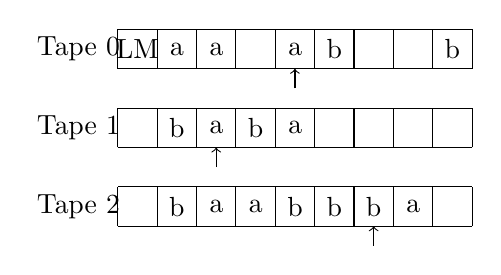
\begin{tikzpicture}[scale=0.5]
\draw (5,10) grid (6,11); %tape 0
\draw (6,10) grid (7,11);
\draw (7,10) grid (8,11);
\draw (8,10) grid (9,11);
\draw (9,10) grid (10,11);
\draw (10,10) grid (11,11);
\draw (11,10) grid (12,11);
\draw (12,10) grid (13,11);
\draw (13,10) grid (14,11);
\draw (5.5,10.5) node {LM}; %tape 0 contents
\draw (6.5,10.5) node {a};
\draw (7.5,10.5) node {a};
%\draw (8.5,10.5) node {a};
\draw (9.5,10.5) node {a};
\draw (10.5,10.5) node {b};
%\draw (11.5,10.35) node {--};
%\draw (12.5,10.35) node {--};
\draw (13.5,10.5) node {b};

\draw[->] (9.5,9.5) -- (9.5,10); %tape 0 head
\draw (4,10.5) node {Tape 0};

\draw (5,8) grid (6,9); %tape 1
\draw (6,8) grid (7,9);
\draw (7,8) grid (8,9);
\draw (8,8) grid (9,9);
\draw (9,8) grid (10,9);
\draw (10,8) grid (11,9);
\draw (11,8) grid (12,9);
\draw (12,8) grid (13,9);
\draw (13,8) grid (14,9);
%\draw (5.5,10.5) node {}; %tape 1 contents
\draw (6.5,8.5) node {b};
\draw (7.5,8.5) node {a};
\draw (8.5,8.5) node {b};
\draw (9.5,8.5) node {a};
%\draw (10.5,10.5) node {b};
%\draw (11.5,10.35) node {--};
%\draw (12.5,10.35) node {--};
%\draw (13.5,8.5) node {\dotss};

\draw[->] (7.5,7.5) -- (7.5,8); %tape 1 head
\draw (4,8.5) node {Tape 1};

\draw (5,6) grid (6,7); %tape 2
\draw (6,6) grid (7,7);
\draw (7,6) grid (8,7);
\draw (8,6) grid (9,7);
\draw (9,6) grid (10,7);
\draw (10,6) grid (11,7);
\draw (11,6) grid (12,7);
\draw (12,6) grid (13,7);
\draw (13,6) grid (14,7);
\draw (5.5,6.5) node {}; %tape 2 contents
\draw (6.5,6.5) node {b};
\draw (7.5,6.5) node {a};
\draw (8.5,6.5) node {a};
\draw (9.5,6.5) node {b};
\draw (10.5,6.5) node {b};
\draw (11.5,6.5) node {b};
\draw (12.5,6.5) node {a};
%\draw (13.5,6.5) node {\dotss};

\draw[->] (11.5,5.5) -- (11.5,6); %tape 2 head
\draw (4,6.5) node {Tape 2};
\end{tikzpicture}
\end{center}
\begin{itemize}
\item<1-> A \tm{} must represent all the information contained in the \mttm{}'s tape configurations

\item<2-> How can this information be represented on a single tape? 

\item<3-> We shall draw inspiration from hard disk technology and imagine that a standard \tm{}'s tape is divided into tracks
    
\item<3-> A k--tape \mttm{} is simulated using 2k tracks

\item<3-> The even tracks, numbered 2j, represent tape j's content in the \mttm{}
    
\item<3-> The odd tracks, numbered 2j+1, capture the head's position on tape j

\end{itemize}
\end{scriptsize}
\end{frame}

\begin{frame}[fragile]
\frametitle{Turing Machine Extensions}
%\framesubtitle{HOMEWORK}
\begin{scriptsize}
\begin{center}
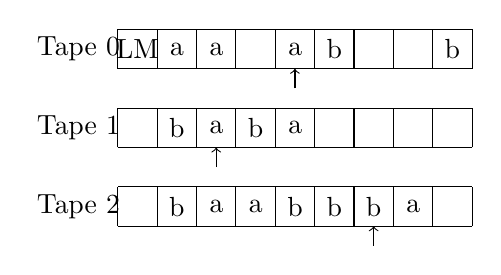
\begin{tikzpicture}[scale=0.5]
\draw (5,10) grid (6,11); %tape 0
\draw (6,10) grid (7,11);
\draw (7,10) grid (8,11);
\draw (8,10) grid (9,11);
\draw (9,10) grid (10,11);
\draw (10,10) grid (11,11);
\draw (11,10) grid (12,11);
\draw (12,10) grid (13,11);
\draw (13,10) grid (14,11);
\draw (5.5,10.5) node {LM}; %tape 0 contents
\draw (6.5,10.5) node {a};
\draw (7.5,10.5) node {a};
%\draw (8.5,10.5) node {a};
\draw (9.5,10.5) node {a};
\draw (10.5,10.5) node {b};
%\draw (11.5,10.35) node {--};
%\draw (12.5,10.35) node {--};
\draw (13.5,10.5) node {b};

\draw[->] (9.5,9.5) -- (9.5,10); %tape 0 head
\draw (4,10.5) node {Tape 0};

\draw (5,8) grid (6,9); %tape 1
\draw (6,8) grid (7,9);
\draw (7,8) grid (8,9);
\draw (8,8) grid (9,9);
\draw (9,8) grid (10,9);
\draw (10,8) grid (11,9);
\draw (11,8) grid (12,9);
\draw (12,8) grid (13,9);
\draw (13,8) grid (14,9);
%\draw (5.5,10.5) node {}; %tape 1 contents
\draw (6.5,8.5) node {b};
\draw (7.5,8.5) node {a};
\draw (8.5,8.5) node {b};
\draw (9.5,8.5) node {a};
%\draw (10.5,10.5) node {b};
%\draw (11.5,10.35) node {--};
%\draw (12.5,10.35) node {--};
%\draw (13.5,8.5) node {\dotss};

\draw[->] (7.5,7.5) -- (7.5,8); %tape 1 head
\draw (4,8.5) node {Tape 1};

\draw (5,6) grid (6,7); %tape 2
\draw (6,6) grid (7,7);
\draw (7,6) grid (8,7);
\draw (8,6) grid (9,7);
\draw (9,6) grid (10,7);
\draw (10,6) grid (11,7);
\draw (11,6) grid (12,7);
\draw (12,6) grid (13,7);
\draw (13,6) grid (14,7);
\draw (5.5,6.5) node {}; %tape 2 contents
\draw (6.5,6.5) node {b};
\draw (7.5,6.5) node {a};
\draw (8.5,6.5) node {a};
\draw (9.5,6.5) node {b};
\draw (10.5,6.5) node {b};
\draw (11.5,6.5) node {b};
\draw (12.5,6.5) node {a};
%\draw (13.5,6.5) node {\dotss};

\draw[->] (11.5,5.5) -- (11.5,6); %tape 2 head
\draw (4,6.5) node {Tape 2};
\end{tikzpicture}
\end{center}

\begin{center}
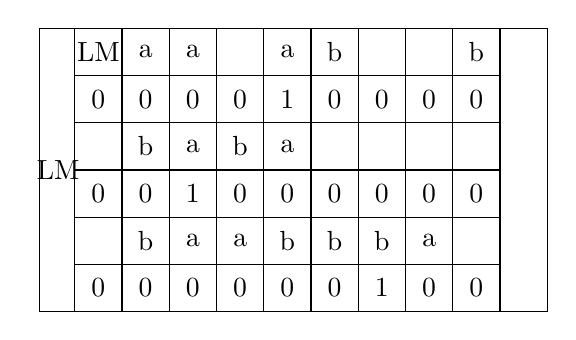
\begin{tikzpicture}[scale=0.6]
\draw (5,10) grid (6,11); %tape 0
\draw (6,10) grid (7,11);
\draw (7,10) grid (8,11);
\draw (8,10) grid (9,11);
\draw (9,10) grid (10,11);
\draw (10,10) grid (11,11);
\draw (11,10) grid (12,11);
\draw (12,10) grid (13,11);
\draw (13,10) grid (14,11);
\draw (5.5,10.5) node {LM}; %tape 0 contents
\draw (6.5,10.5) node {a};
\draw (7.5,10.5) node {a};
%\draw (8.5,10.5) node {a};
\draw (9.5,10.5) node {a};
\draw (10.5,10.5) node {b};
%\draw (11.5,10.35) node {--};
%\draw (12.5,10.35) node {--};
\draw (13.5,10.5) node {b};

\draw (5,9) grid (6,10); %tape 0 head
\draw (6,9) grid (7,10);
\draw (7,9) grid (8,10);
\draw (8,9) grid (9,10);
\draw (9,9) grid (10,10);
\draw (10,9) grid (11,10);
\draw (11,9) grid (12,10);
\draw (12,9) grid (13,10);
\draw (13,9) grid (14,10);
\draw (5.5,9.5) node {0}; %tape 0 heads contents
\draw (6.5,9.5) node {0};
\draw (7.5,9.5) node {0};
\draw (8.5,9.5) node {0};
\draw (9.5,9.5) node {1};
\draw (10.5,9.5) node {0};
\draw (11.5,9.5) node {0};
\draw (12.5,9.5) node {0};
\draw (13.5,9.5) node {0};



\draw (5,8) grid (6,9); %tape 1
\draw (6,8) grid (7,9);
\draw (7,8) grid (8,9);
\draw (8,8) grid (9,9);
\draw (9,8) grid (10,9);
\draw (10,8) grid (11,9);
\draw (11,8) grid (12,9);
\draw (12,8) grid (13,9);
\draw (13,8) grid (14,9);
%\draw (5.5,10.5) node {}; %tape 1 contents
\draw (6.5,8.5) node {b};
\draw (7.5,8.5) node {a};
\draw (8.5,8.5) node {b};
\draw (9.5,8.5) node {a};
%\draw (10.5,10.5) node {b};
%\draw (11.5,10.35) node {--};
%\draw (12.5,10.35) node {--};
%\draw (13.5,8.5) node {\dotss};

\draw (5,7) grid (6,8); %tape 1 head
\draw (6,7) grid (7,8);
\draw (7,7) grid (8,8);
\draw (8,7) grid (9,8);
\draw (9,7) grid (10,8);
\draw (10,7) grid (11,8);
\draw (11,7) grid (12,8);
\draw (12,7) grid (13,8);
\draw (13,7) grid (14,8);
\draw (5.5,7.5) node {0}; %tape 1 heads contents
\draw (6.5,7.5) node {0};
\draw (7.5,7.5) node {1};
\draw (8.5,7.5) node {0};
\draw (9.5,7.5) node {0};
\draw (10.5,7.5) node {0};
\draw (11.5,7.5) node {0};
\draw (12.5,7.5) node {0};
\draw (13.5,7.5) node {0};



\draw (5,6) grid (6,7); %tape 2
\draw (6,6) grid (7,7);
\draw (7,6) grid (8,7);
\draw (8,6) grid (9,7);
\draw (9,6) grid (10,7);
\draw (10,6) grid (11,7);
\draw (11,6) grid (12,7);
\draw (12,6) grid (13,7);
\draw (13,6) grid (14,7);
\draw (5.5,6.5) node {}; %tape 2 contents
\draw (6.5,6.5) node {b};
\draw (7.5,6.5) node {a};
\draw (8.5,6.5) node {a};
\draw (9.5,6.5) node {b};
\draw (10.5,6.5) node {b};
\draw (11.5,6.5) node {b};
\draw (12.5,6.5) node {a};
%\draw (13.5,6.5) node {\dotss};

\draw (5,5) grid (6,6); %tape 1 head
\draw (6,5) grid (7,6);
\draw (7,5) grid (8,6);
\draw (8,5) grid (9,6);
\draw (9,5) grid (10,6);
\draw (10,5) grid (11,6);
\draw (11,5) grid (12,6);
\draw (12,5) grid (13,6);
\draw (13,5) grid (14,6);
\draw (5.5,5.5) node {0}; %tape 1 heads contents
\draw (6.5,5.5) node {0};
\draw (7.5,5.5) node {0};
\draw (8.5,5.5) node {0};
\draw (9.5,5.5) node {0};
\draw (10.5,5.5) node {0};
\draw (11.5,5.5) node {1};
\draw (12.5,5.5) node {0};
\draw (13.5,5.5) node {0};

\draw (4.25,5) rectangle (5,11);
\draw (4.65,8) node {LM};

\draw (14,5) rectangle (15,11);
%\draw (14.75,5) rectangle (15.5,11);

\end{tikzpicture}
\end{center}
\end{scriptsize}
\end{frame}

\begin{frame}[fragile]
\frametitle{Turing Machine Extensions}
%\framesubtitle{HOMEWORK}
\begin{scriptsize}
\begin{center}
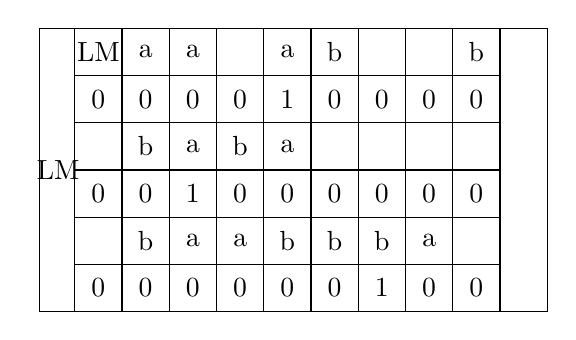
\begin{tikzpicture}[scale=0.6]
\draw (5,10) grid (6,11); %tape 0
\draw (6,10) grid (7,11);
\draw (7,10) grid (8,11);
\draw (8,10) grid (9,11);
\draw (9,10) grid (10,11);
\draw (10,10) grid (11,11);
\draw (11,10) grid (12,11);
\draw (12,10) grid (13,11);
\draw (13,10) grid (14,11);
\draw (5.5,10.5) node {LM}; %tape 0 contents
\draw (6.5,10.5) node {a};
\draw (7.5,10.5) node {a};
%\draw (8.5,10.5) node {a};
\draw (9.5,10.5) node {a};
\draw (10.5,10.5) node {b};
%\draw (11.5,10.35) node {--};
%\draw (12.5,10.35) node {--};
\draw (13.5,10.5) node {b};

\draw (5,9) grid (6,10); %tape 0 head
\draw (6,9) grid (7,10);
\draw (7,9) grid (8,10);
\draw (8,9) grid (9,10);
\draw (9,9) grid (10,10);
\draw (10,9) grid (11,10);
\draw (11,9) grid (12,10);
\draw (12,9) grid (13,10);
\draw (13,9) grid (14,10);
\draw (5.5,9.5) node {0}; %tape 0 heads contents
\draw (6.5,9.5) node {0};
\draw (7.5,9.5) node {0};
\draw (8.5,9.5) node {0};
\draw (9.5,9.5) node {1};
\draw (10.5,9.5) node {0};
\draw (11.5,9.5) node {0};
\draw (12.5,9.5) node {0};
\draw (13.5,9.5) node {0};



\draw (5,8) grid (6,9); %tape 1
\draw (6,8) grid (7,9);
\draw (7,8) grid (8,9);
\draw (8,8) grid (9,9);
\draw (9,8) grid (10,9);
\draw (10,8) grid (11,9);
\draw (11,8) grid (12,9);
\draw (12,8) grid (13,9);
\draw (13,8) grid (14,9);
%\draw (5.5,10.5) node {}; %tape 1 contents
\draw (6.5,8.5) node {b};
\draw (7.5,8.5) node {a};
\draw (8.5,8.5) node {b};
\draw (9.5,8.5) node {a};
%\draw (10.5,10.5) node {b};
%\draw (11.5,10.35) node {--};
%\draw (12.5,10.35) node {--};
%\draw (13.5,8.5) node {\dotss};

\draw (5,7) grid (6,8); %tape 1 head
\draw (6,7) grid (7,8);
\draw (7,7) grid (8,8);
\draw (8,7) grid (9,8);
\draw (9,7) grid (10,8);
\draw (10,7) grid (11,8);
\draw (11,7) grid (12,8);
\draw (12,7) grid (13,8);
\draw (13,7) grid (14,8);
\draw (5.5,7.5) node {0}; %tape 1 heads contents
\draw (6.5,7.5) node {0};
\draw (7.5,7.5) node {1};
\draw (8.5,7.5) node {0};
\draw (9.5,7.5) node {0};
\draw (10.5,7.5) node {0};
\draw (11.5,7.5) node {0};
\draw (12.5,7.5) node {0};
\draw (13.5,7.5) node {0};



\draw (5,6) grid (6,7); %tape 2
\draw (6,6) grid (7,7);
\draw (7,6) grid (8,7);
\draw (8,6) grid (9,7);
\draw (9,6) grid (10,7);
\draw (10,6) grid (11,7);
\draw (11,6) grid (12,7);
\draw (12,6) grid (13,7);
\draw (13,6) grid (14,7);
\draw (5.5,6.5) node {}; %tape 2 contents
\draw (6.5,6.5) node {b};
\draw (7.5,6.5) node {a};
\draw (8.5,6.5) node {a};
\draw (9.5,6.5) node {b};
\draw (10.5,6.5) node {b};
\draw (11.5,6.5) node {b};
\draw (12.5,6.5) node {a};
%\draw (13.5,6.5) node {\dotss};

\draw (5,5) grid (6,6); %tape 1 head
\draw (6,5) grid (7,6);
\draw (7,5) grid (8,6);
\draw (8,5) grid (9,6);
\draw (9,5) grid (10,6);
\draw (10,5) grid (11,6);
\draw (11,5) grid (12,6);
\draw (12,5) grid (13,6);
\draw (13,5) grid (14,6);
\draw (5.5,5.5) node {0}; %tape 1 heads contents
\draw (6.5,5.5) node {0};
\draw (7.5,5.5) node {0};
\draw (8.5,5.5) node {0};
\draw (9.5,5.5) node {0};
\draw (10.5,5.5) node {0};
\draw (11.5,5.5) node {1};
\draw (12.5,5.5) node {0};
\draw (13.5,5.5) node {0};

\draw (4.25,5) rectangle (5,11);
\draw (4.65,8) node {LM};

\draw (14,5) rectangle (15,11);
%\draw (14.75,5) rectangle (15.5,11);

\end{tikzpicture}
\end{center}

\begin{center}
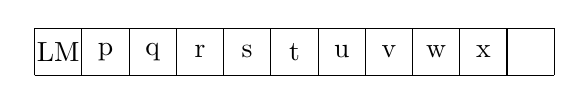
\begin{tikzpicture}[scale=0.6]
\draw (4,10) grid (5,11);
\draw (5,10) grid (6,11); %tape
\draw (6,10) grid (7,11);
\draw (7,10) grid (8,11);
\draw (8,10) grid (9,11);
\draw (9,10) grid (10,11);
\draw (10,10) grid (11,11);
\draw (11,10) grid (12,11);
\draw (12,10) grid (13,11);
\draw (13,10) grid (14,11);
\draw (14,10) grid (15,11);
\draw (4.5,10.5) node {LM};
\draw (5.5,10.5) node {p}; %tape contents
\draw (6.5,10.5) node {q};
\draw (7.5,10.5) node {r};
\draw (8.5,10.5) node {s};
\draw (9.5,10.5) node {t};
\draw (10.5,10.5) node {u};
\draw (11.5,10.5) node {v};
\draw (12.5,10.5) node {w};
\draw (13.5,10.5) node {x};
\end{tikzpicture}
\end{center}
\begin{itemize}
\item<1-> The division into tracks, of course, is an abstraction that must be implemented
     
\item<1-> The simulating \tm{} must contain the \mttm{}'s alphabet to receive the same 
    
\item<1-> Each position in the simulating \tm{}'s tape is either \texttt{LM}, \texttt{BLANK}, or a symbol representing an element in (\sig $\times$ \{0 1\})$^{\texttt{k}}$,
    
\item<1-> The simulating \tm{}'s alphabet must have a symbol for each possible column in the track representation of the multiple tapes

\end{itemize}
\end{scriptsize}
\end{frame}

\begin{frame}[fragile]
\frametitle{Turing Machine Extensions}
%\framesubtitle{HOMEWORK}
\begin{tiny}
\begin{itemize}
\begin{theorem}
\label{mttm-thm}
Let M = (make-mttm K \sig{} S F R n [Y]). There exists a Turing machine, M\quot{} = (make-tm K\quot{} \sig{}\quot{} S\quot{} F R\quot{} [Y]), that simulates M.
\end{theorem}

\item<2->
\begin{proof} 
\begin{itemize}
\item<2-> \tiny Assume the precondition for M is: PRE: tape 0 = (LM BLANK w) and t0h = 1

\item<3-> \tiny Three primary phases M\quot{} operates in:
\begin{alltt}
1. Make M\quot{}'s tape represent M's initial configuration.
   a. Shift w to the right one space
   b. To represent the beginning of the k tapes and write \sig{}\quot{}'s symbol for:
      LM
      0
      BLANK
      1
      \vdotss
   This symbol captures: head on tape 0 is not on the left-end marker 
   c. Move right to capture tape 0's head position by writing symbol for:
      BLANK
      1
      BLANK
      0
      \vdotss
   d. Move right until a blank is read. For each e\(\in\)\sig{} read, write \sig{}\quot{}'s symbol for:
      e
      0
      BLANK
      0
      \vdotss
\end{alltt}

\end{itemize}
\end{proof}

\end{itemize}
\end{tiny}
\end{frame}

\begin{frame}[fragile]
\frametitle{Turing Machine Extensions}
%\framesubtitle{HOMEWORK}
\begin{tiny}
\begin{itemize}
\begin{theorem}
\label{mttm-thm}
Let M = (make-mttm K \sig{} S F R n [Y]). There exists a Turing machine, M\quot{} = (make-tm K\quot{} \sig{}\quot{} S\quot{} F R\quot{} [Y]), that simulates M.
\end{theorem}

\item<1->
\begin{proof} 
\begin{itemize}
\item<1-> \tiny Assume the precondition for M is: PRE: tape 0 = (LM BLANK w) and t0h = 1

\item<1-> \tiny Three primary phases M\quot{} operates in:
\begin{alltt}
2. Simulate M. For each transition that would be made by M, M\quot{} starts on the 
   first blank that is not encoded into tracks and performs the 
   following operations:

        1. Move left and determine what would be read by each of M's head as 
           described in the design idea and return the head to the first
           blank that is not encoded into tracks.
        
        2. Move left to update the tracks as M would update its tapes 
           and heads.
\end{alltt}

\end{itemize}
\end{proof}

\item<2-> \tiny Many design choices are  not described for phase 2, but it ought to be clear that M\quot{} simulates M
     
\item<2-> \tiny M\quot{} performs many transitions to simulate one transition performed by M
\end{itemize}
\end{tiny}
\end{frame}

\begin{frame}[fragile]
\frametitle{Turing Machine Extensions}
%\framesubtitle{HOMEWORK}
\begin{tiny}
\begin{itemize}
\begin{theorem}
\label{mttm-thm}
Let M = (make-mttm K \sig{} S F R n [Y]). There exists a Turing machine, M\quot{} = (make-tm K\quot{} \sig{}\quot{} S\quot{} F R\quot{} [Y]), that simulates M.
\end{theorem}

\item<1->
\begin{proof} 
\begin{itemize}
\item<1-> \tiny Assume the precondition for M is: PRE: tape 0 = (LM BLANK w) and t0h = 1

\item<1-> \tiny Three primary phases M\quot{} operates in:
\begin{alltt}
3. If M would halt, convert the contents of the tape (i.e., M\quot{}'s tape) to 
   single track
  a. Ignores all tracks except tracks 0 and 1
  b. The content of track 0 is written to the tape
  c. the head is placed at the position indicated by track 1
  d. M\quot{} moves to the state M would halt in and halts itself.
\end{alltt}

\end{itemize}
\end{proof}

\end{itemize}
\end{tiny}
\end{frame}


\begin{frame}[fragile]
\frametitle{Turing Machine Extensions}
%\framesubtitle{HOMEWORK}
\begin{scriptsize}
\begin{itemize}
\item<1-> Does a Turing machine with one tape and multiple heads operating on the tape provide us with more computational power? 
    
\item<1-> Each head operates independently of the others

\item<1-> If a head moves right or left it does not interfere with other heads
    
\item<1-> A synchronization mechanism must be implemented when two or more heads try to write to the same tape position (assume it exists)

\item<1-> How can a standard \tm{} simulate a Turing machine with one tape and multiple heads? 
    
\item<2-> A representation strategy similar to the one used to simulate multiple tapes may be used
    
\item<2-> The standard Turing machine operates on an encoded multiple track tape
    
\item<2-> The first track represents the input tape and the rest of the tracks record each head's position
    
\item<3-> To simulate one step of the multiple heads machine, the standard \tm{} scans the tape twice
    
\item<3-> The first to determine the elements read by each of the multiple heads
    
\item<3-> The second to simulate the action of each head (i.e., mutate the first track or move the head)

\end{itemize}
\end{scriptsize}
\end{frame}

\begin{frame}[fragile]
\frametitle{Turing Machine Extensions}
%\framesubtitle{HOMEWORK}
\begin{scriptsize}
\begin{itemize}
\item<1-> Is a Turing machine with a tape that is infinite both to the right and the left more powerful than a standard Turing machine? 
    
\item<1-> In such a machine, at the beginning only the input is written on the tape and the rest of the positions are blank
    
\item<1-> There is no left-end marker in such a machine.

\item<2-> A two-way infinite input tape Turing machine may be simulated by a 2-tape \mttm{}
    
\item<2-> Initially, the first tape contains the input and the second tape is blank
    
\item<2-> During a computation, if the head of the two-way infinite input tape Turing machine is on the first element of the input or to right of it then the standard \tm{} operates on tape 0
    
\item<2-> Otherwise, it operates on tape 1 where the elements are written in reversed order (right and left moves are simulated, respectively, by left and right moves on tape 1)

\end{itemize}
\end{scriptsize}
\end{frame}


\begin{frame}[fragile]
\frametitle{Turing Machine Extensions}
\framesubtitle{FINAL EXAM PROJECT}
\begin{scriptsize}
\begin{itemize}
\item<1-> Design, build, validate, and verify a constructor that given a \pda{} builds a \mttm{} that simulates it
    
\item<1-> Problems: 6--12

\end{itemize}
\end{scriptsize}
\end{frame}

\section{Context-Sensitive Grammars}

\begin{frame}[fragile]
\frametitle{Context-Sensitive Grammars}
%\framesubtitle{HOMEWORK}
\begin{scriptsize}
\begin{itemize}
\item<1-> Turing machines are automata that are capable of deciding languages that are not context-free
    
\item<1-> We have seen that less powerful automata, \dfa{}s and \pda{}s, have language generator counterparts called, respectively, regular grammars/expressions and context-free grammars
    
\item<1-> Are there grammars for the languages that Turing machines decide or semidecide?

\item<2-> We shall now explore \emph{context-sensitive grammars} (\csg{}s). 
    
    
\item<2-> Unlike previous grammars, the left hand side of a rule may consist of any number of terminal and nonterminal symbols as long as there is at least one nonterminal symbol
    
\item<2-> The length of a partially generated word may arbitrarily decrease in a single step

\end{itemize}
\end{scriptsize}
\end{frame}

\begin{frame}[fragile]
\frametitle{Context-Sensitive Grammars}
%\framesubtitle{HOMEWORK}
\begin{scriptsize}
\begin{itemize}
\item<1-> Formally:
\begin{alltt}
  A context-free grammar is an instance of (make-csg N \sig R S)
\end{alltt}

\item<2-> Each production rule is of the form:
\begin{alltt}
     (N \(\cup\) \sig{})\(\sp{*}\)N(N \(\cup\) \sig{})\(\sp{*}\) \arrow{} (N \(\cup\) \sig{})\(\sp{*}\)

     (N \(\cup\) \sig{})\(\sp{*}\)N(N \(\cup\) \sig{})\(\sp{*}\) \arrow{} EMP
\end{alltt}

\item<2-> The set of regular grammars and the set of context-free grammars are both proper subsets of the set of context-sensitive grammars

\item<3-> \texttt{L(G)} denotes the language generated by \texttt{G}: \texttt{\{w $|$ w$\in$\sig$^*$ $\wedge$ S \arrow$^*_G$ w\}}
     
\item<3-> A language, \texttt{L}, is context-sensitive if \texttt{L = L(G)} for some context-sensitive grammar \texttt{G}

\end{itemize}
\end{scriptsize}
\end{frame}

\begin{frame}[fragile]
\frametitle{Context-Sensitive Grammars}
%\framesubtitle{HOMEWORK}
\begin{scriptsize}
\begin{itemize}
\item<1-> \texttt{L} = \texttt{a$^{\texttt{n}}$b$^{\texttt{n}}$c$^{\texttt{n}}$}
    
\item<2-> We shall design the grammar following the steps of the design recipe
     
\item<2-> The syntactic category represented by a nonterminal may be less clear-cut than their counterparts in \cfg{}s and \rg{}s
    
\item<2-> For instance, a nonterminal may not represent a syntactic category on its own given that it may only generate something in the proper context
    
\item<2-> It is sometimes useful to think of a nonterminal as a promise to generate a desired subword in the proper context or as partially defining a syntactic category
    
\item<3-> Finding a derivation may take very long making some tests unpractical
    
\item<3-> Attempting to find derivations for a word not in the language may take forever. Again, this is especially true when the grammar uses nondeterminism
    
\item<3-> Unlike for \rg{}s and \cfg{}s, there is no algorithm to distinguish when a search has become futile. This has rather important consequences for us as programmers
    
\item<3-> Careful design is of paramount importance

\end{itemize}
\end{scriptsize}
\end{frame}

\begin{frame}[fragile]
\frametitle{Context-Sensitive Grammars}
%\framesubtitle{HOMEWORK}
\begin{scriptsize}
\begin{itemize}
\item<1-> Design Idea

\item<1-> \texttt{A}, \texttt{B}, and \texttt{C} represent promises to generate \texttt{a}s, \texttt{b}s, and \texttt{c}s in the proper context
    
\item<1-> This generation ends with a nonterminal, say \texttt{G}, that represents a promise to generate \texttt{c}s in the proper context
     
\item<1-> The proper context, of course, is that all the \texttt{A}s must be before the all the \texttt{B}s which must be before all the \texttt{C}s with the \texttt{G} at the end
     
\item<2-> Before generating terminal symbols, the grammar nondeterministically rearranges the \texttt{A}s, \texttt{B}s, and \texttt{C}s in the right order 
    
\item<3-> Finally, the grammar traverses the partially generated word, from right to left, to generate the \texttt{c}s
    
\item<3-> If there is \texttt{CG} in the partially generated word then the \texttt{G} may be moved left and a \texttt{c} is generated: \texttt{CG} generates \texttt{Gc}
    
\item<4-> After the last \texttt{c} is generated, the grammar generates a nonterminal, say \texttt{H}, that represents a promise to generate the \texttt{b}s in the proper context and continues the traversal to generate all the \texttt{b}s

\item<5-> When the last \texttt{b} is generated, the grammar generates a nonterminal, say \texttt{I}, that represents a promise to generate the \texttt{a}s in the proper context and continues the traversal to generate all the \texttt{a}s
     
\item<6-> When the last \texttt{a} is generated \texttt{I} generates \texttt{EMP} and the derivation is done

\end{itemize}
\end{scriptsize}
\end{frame}

\begin{frame}[fragile]
\frametitle{Context-Sensitive Grammars}
%\framesubtitle{HOMEWORK}
\begin{tiny}
\begin{itemize}
\item<1-> Design Idea

\item<1-> Consider the derivation for \texttt{aaabbbccc}

\item<1-> Nondeterministically generate \texttt{ABC} three times ending with \texttt{G}:
\begin{alltt}
     ABCABCABCG
\end{alltt}


\item<2-> Rearrange the \texttt{A}s, \texttt{B}s, and \texttt{C}s to be in the right order:
\begin{alltt}
     AAABBBCCCG
\end{alltt}

\item<3-> Generate the \texttt{c}s:
\begin{alltt}
     AAABBBCCGc
     AAABBBCGcc
     AAABBBGccc
\end{alltt}

\item<4-> Nondeterministically generates an \texttt{H} from \texttt{G}:
\begin{alltt}
     AAABBBHccc
\end{alltt}

\item<5-> Generate \texttt{b}s:
\begin{alltt}
     AAABBHbccc
     AAABHbbccc
     AAAHbbbccc
\end{alltt}


\item<6-> Nondeterministically generates an \texttt{I}:
\begin{alltt}
     AAAIbbbccc
\end{alltt}

\item<7-> Generate \texttt{a}s:
\begin{alltt}
     AAIabbbccc
     AIaabbbccc
     Iaaabbbccc
\end{alltt}

\item<8-> Nondeterministically generate \texttt{EMP}:
\begin{alltt}
     aaabbbccc
\end{alltt}

\end{itemize}
\end{tiny}
\end{frame}

\begin{frame}[fragile]
\frametitle{Context-Sensitive Grammars}
%\framesubtitle{HOMEWORK}
\begin{scriptsize}
\begin{itemize}
\item<1-> A descriptive name for the grammar is \texttt{anbncn}

\item<1-> The alphabet is \texttt{\{a b c\}}.

\item<2-> \texttt{A} and \texttt{I} together may generate an \texttt{a} in the context \texttt{AI}
    
\item<3-> \texttt{B} and \texttt{H} together may generate a \texttt{b} in the context \texttt{BH}
    
\item<4-> \texttt{C} and \texttt{G} together may generate an \texttt{a} in the context \texttt{CG}
    
\item<5-> We document the syntactic categories as follows:
\begin{alltt}
     ;; Syntactic Categories
     ;; S: generates words in a^nb^nc^n
     ;; A,I: A promise to generate an a in the context AI
     ;; B,H: A promise to generate an b in the context BH
     ;; C,G: A promise to generate an c in the context CG
\end{alltt}

\end{itemize}
\end{scriptsize}
\end{frame}

\begin{frame}[fragile]
\frametitle{Context-Sensitive Grammars}
%\framesubtitle{HOMEWORK}
\begin{scriptsize}
\begin{itemize}
\item<1-> Production Rules

\item<1-> \texttt{S} needs to generate an arbitrary number of \texttt{ABC} and needs to generate \texttt{G}:
\begin{alltt}
     (S ,ARROW ,EMP)
     (S ,ARROW ABCS)  \textcolor{blue}{S \(\Rightarrow\) |A|=|B|=|C|}
     (S ,ARROW G)     
\end{alltt}

\item<2-> To rearrange the \texttt{A}s, \texttt{B}s, and \texttt{C}s, nonterminals out of order are put in the right order:
\begin{alltt}
     (BA ,ARROW AB)
     (CA ,ARROW AC)
     (CB ,ARROW BC)
\end{alltt}

\item<3-> \texttt{C} and \texttt{G} are used to generate \texttt{c}s, move \texttt{G} right to left, and nondeterministically generate an \texttt{H}:
\begin{alltt}
     (CG ,ARROW Gc)  \textcolor{blue}{G \(\Rightarrow\) only c\(\sp{*}\) to the right}
     (BG  ,ARROW BH)
\end{alltt}

\item<4-> \texttt{B} and \texttt{H} are used to generate \texttt{b}s, move \texttt{H} right to left, and nondeterministically generate an \texttt{I}:
\begin{alltt}
     (BH ,ARROW Hb)  \textcolor{blue}{H \(\Rightarrow\) only b\(\sp{*}\)c\(\sp{+}\) to the right}
     (AH ,ARROW AI)
\end{alltt}

\item<5-> \texttt{A} and \texttt{I} are used to generate \texttt{a}s, move \texttt{I} right to left, and nondeterministically generate \texttt{EMP}:
\begin{alltt}
     (AI ,ARROW Ia)  \textcolor{blue}{I \(\Rightarrow\) only a\(\sp{*}\)b\(\sp{+}\)c\(\sp{+}\) to the right}
     (I ,ARROW ,EMP)
\end{alltt}

\end{itemize}
\end{scriptsize}
\end{frame}

\begin{frame}[fragile]
\frametitle{Context-Sensitive Grammars}
%\framesubtitle{HOMEWORK}
\begin{tiny}
\begin{itemize}
\item<1-> Some trial and error may be needed to make sure tests run in a reasonable amount of time
     
\item<1-> A good heuristic is to test relatively short words that are in the language:
\begin{alltt}
     (check-derive? anbncn \quot{}(a b c) \quot{}(a a b b c c) \quot{}())
     ;; (check=not=derive? anbncn \quot{}(a) \quot{}(b) \quot{}(c) \quot{}(c b a) \quot{}(a a b b c c c))
\end{alltt}

\end{itemize}
\end{tiny}
\end{frame}

\begin{frame}[fragile]
\frametitle{Context-Sensitive Grammars}
%\framesubtitle{HOMEWORK}
\begin{scriptsize}
\begin{itemize}
\item<1-> Writing tests using words that are not in \texttt{L} is ill-advised in this case
     
\item<1-> The search space for finding a derivation may be visualized as a tree
    
\item<1-> Consider trying to find a derivation for \texttt{aa}:
\begin{center}
\scalebox{0.7}{ 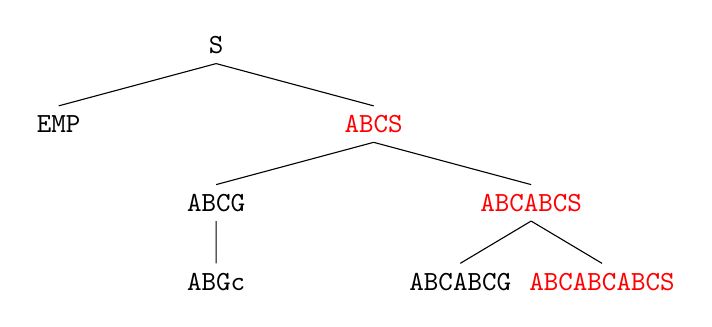
\begin{tikzpicture}[level distance=1.0cm,level 1/.style={sibling distance=4cm},level 2/.style={sibling distance=4cm},level 3/.style={sibling distance=1.8cm}]
    \node {\texttt{S}}
      child {node {\texttt{EMP}}}
      child {node {\texttt{\textcolor{red}{ABCS}}}
        child {node {\texttt{ABCG}}
          child {node {\texttt{ABGc}}}}
        child {node {\texttt{\textcolor{red}{ABCABCS}}}
          child {node {\texttt{ABCABCG}}}
          child {node {\texttt{\textcolor{red}{ABCABCABCS}}}}}};
    \end{tikzpicture}}
\end{center}

\item<1-> The partially generated word down rightmost branches is always made longer and leads to an infinite search
    
\item<1-> We are unable to write tests using words that are not in \texttt{L}
    
\item<2-> \texttt{grammar-test} may easily be caught in an infinite recursion when used to test a \csg{}
    
\item<2-> Its use with \csg{}s is disabled in \fsm

\end{itemize}
\end{scriptsize}
\end{frame}

\begin{frame}[fragile]
\frametitle{Context-Sensitive Grammars}
%\framesubtitle{HOMEWORK}
\begin{scriptsize}
\begin{itemize}
\item<1-> To prove correctness think of the derivation process as follows:
\begin{alltt}
     while (contains-nonterminals? yield)
         apply-rule()
\end{alltt}

\item<2-> Develop a predicate for the loop invariant

\item<3->
\begin{itemize}
 \item $|$\texttt{A} and \texttt{a}$|$=$|$\texttt{B} and \texttt{b}$|$=$|$\texttt{C} and \texttt{c}$|$
 \item \texttt{S}$\in$\texttt{yield} $\Rightarrow$ \texttt{yield} ends with \texttt{S}
 \item \texttt{G}$\in$\texttt{yield} $\Rightarrow$ \texttt{yield} ends with \texttt{G}\texttt{c}$^{\texttt{*}}$
 \item \texttt{H}$\in$\texttt{yield} $\Rightarrow$ \texttt{yield} ends with \texttt{H}\texttt{b}$^{\texttt{*}}$\texttt{c}$^{\texttt{+}}$
 \item \texttt{I}$\in$\texttt{yield} $\Rightarrow$ \texttt{yield} ends with \texttt{I}\texttt{a}$^{\texttt{*}}$\texttt{b}$^{\texttt{+}}$\texttt{c}$^{\texttt{+}}$
 \item \texttt{yield}$\in$$\Sigma^{\texttt{*}}$ $\Rightarrow$ \texttt{yield}$\in$L
\end{itemize}

\end{itemize}
\end{scriptsize}
\end{frame}



\begin{frame}[fragile]
\frametitle{Context-Sensitive Grammars}
%\framesubtitle{HOMEWORK}
\begin{scriptsize}
\begin{itemize}
\item<1-> 
\begin{alltt}
;; (listof (N \(\cup{}\) \(\Sigma\)) \(\rightarrow\) Boolean
;; Purpose: Determine if loop invariant holds for the given yield
(define (anbncn-inv yield)
  (and (equal-num-abc? yield) \textcolor{blue}{equal number A/a,B/b,C/c}
       (implies (member \quot{}S yield) (S-INV yield))
       (implies (member \quot{}G yield) (G-INV yield))
       (implies (member \quot{}H yield) (H-INV yield))
       (implies (member \quot{}I yield) (I-INV yield))
       (implies (no-nt? yield)    (in-lang? yield))))
\end{alltt}

\item<2->
\begin{alltt}
(define (S-INV yield) (eq? (last yield) \quot{}S))
\end{alltt}

\item<3->
\begin{alltt}
(define (G-INV yield) \textcolor{blue}{Only c's right of G}
    (= (count (lambda (x) (not (eq? \quot{}c x)))
              (rest (dropf yield (lambda (x) (not (eq? \quot{}G x))))))
       0))
\end{alltt}

\item<4->
\begin{alltt}
(define (H-INV yield) \textcolor{blue}{Only b's and c's right of H}
    (let* ([bs-and-cs (rest (dropf yield 
                                   (lambda (x) (not (eq? \quot{}H x)))))]
           [cs (dropf bs-and-cs (lambda (x) (eq? x \quot{}b)))])
      (andmap (lambda (x) (eq? x \quot{}c)) cs)))
\end{alltt}

\end{itemize}
\end{scriptsize}
\end{frame}

\begin{frame}[fragile]
\frametitle{Context-Sensitive Grammars}
%\framesubtitle{HOMEWORK}
\begin{scriptsize}
\begin{itemize}
\item<1-> 
\begin{alltt}
(define (I-INV yield)
    (let* ([as-bs-cs (rest (dropf yield (lambda (x) (not (eq? \quot{}I x)))))]
           [bs-and-cs (dropf as-bs-cs (lambda (x) (eq? \quot{}a x)))]
           [cs (dropf bs-and-cs (lambda (x) (eq? x \quot{}b)))])
      (andmap (lambda (x) (eq? \quot{}c x)) cs)))
\end{alltt}

\item<2-> 
\begin{alltt}
(define (in-lang? yield)
    (let* ([as (takef yield (lambda (x) (eq? \quot{}a x)))]
           [bs-and-cs (dropf yield (lambda (x) (eq? \quot{}a x)))]
           [bs (takef bs-and-cs (lambda (x) (eq? \quot{}b x)))]
           [cs (takef (dropf bs-and-cs (lambda (x) (eq? x \quot{}b))) (lambda (x) (eq? \quot{}c x)))])
      (= (length as) (length bs) (length cs))))
\end{alltt}

\item<3-> 
\begin{alltt}
(define (equal-num-abc? word)
    (= (+ (count (lambda (x) (eq? \quot{}A x)) word)
          (count (lambda (x) (eq? \quot{}a x)) word))
       (+ (count (lambda (x) (eq? \quot{}B x)) word)
          (count (lambda (x) (eq? \quot{}b x)) word))
       (+ (count (lambda (x) (eq? \quot{}C x)) word)
          (count (lambda (x) (eq? \quot{}c x)) word))))
\end{alltt}

\item<4-> 
\begin{alltt}
(define (no-nt? yield)
    (andmap (lambda (x) (member x (grammar-sigma anbncn))) yield))
\end{alltt}

\end{itemize}
\end{scriptsize}
\end{frame}


\begin{frame}[fragile]
\frametitle{Context-Sensitive Grammars}
%\framesubtitle{HOMEWORK}
\begin{scriptsize}
\begin{itemize}
\item<1-> Proof by induction on n=number of derivation steps
\begin{alltt}
Base case:
When derivation starts, yield=S. 
S-INV holds a S is the rightmost element of the yield) \(\wedge\)
the number of As, as, Bs, bs, Cs, and cs are all  0 \(\wedge\)
other implications are true (i.e., false \(\Rightarrow\) X is true)
\end{alltt}

\item<2-> Inductive Step
\begin{alltt}
Assume: INV holds for n=k
  Show: INV holds for n=k+1
\end{alltt}

\item<3-> S $\rightarrow$ EMP
\begin{alltt}
By inductive hypothesis INV holds
After applying this production rule: 
the number of As, as, Bs, bs, Cs, and cs are all  0 \(\wedge\)
(implies (no-nt? yield) (in-lang? yield)) holds \(\wedge\)
other implications are true (i.e., false \(\Rightarrow\) X is true)
\end{alltt}

\item<4-> S $\rightarrow$ ABCS
\begin{alltt}
By inductive hypothesis INV holds
After applying this production rule: 
|A \& a|=|B & b|=|C \& c| \(\wedge\)
S ends the yield \(\wedge\)
other implications are true (i.e., false \(\Rightarrow\) X is true)
\end{alltt}

\end{itemize}
\end{scriptsize}
\end{frame}

\begin{frame}[fragile]
\frametitle{Context-Sensitive Grammars}
%\framesubtitle{HOMEWORK}
\begin{scriptsize}
\begin{itemize}
\item<1-> BA \(\rightarrow\) AB, CB \(\rightarrow\) BC, CA \(\rightarrow\) AC
\begin{alltt}
By inductive hypothesis INV holds
After applying any of these production rules: 
INV holds because only the ordering of A, B, \& C change
\end{alltt}

\item<2-> S \(\rightarrow\) G
\begin{alltt}
By inductive hypothesis INV holds
After applying this production rule: 
|A \& a|=|B & b|=|C \& c| \(\wedge\)
Everything to the right of G is c \(\wedge\)
other implications are true (i.e., false \(\Rightarrow\) X is true)
\end{alltt}

\item<3-> CG \(\rightarrow\) Gc
\begin{alltt}
By inductive hypothesis INV holds
After applying this production rule: 
|A \& a|=|B & b|=|C \& c| \(\wedge\)
Everything to the right of G is c\(\sp{+}\) \(\wedge\)
other implications are true (i.e., false \(\Rightarrow\) X is true)
\end{alltt}

\item<4-> BG \(\rightarrow\) BH
\begin{alltt}
By inductive hypothesis INV holds
After applying this production rule: 
|A \& a|=|B & b|=|C \& c| \(\wedge\)
Everything to the right of H is b\(\sp{*}\)c\(\sp{+}\) \(\wedge\)
other implications are true (i.e., false \(\Rightarrow\) X is true)
\end{alltt}

\end{itemize}
\end{scriptsize}
\end{frame}


\begin{frame}[fragile]
\frametitle{Context-Sensitive Grammars}
%\framesubtitle{HOMEWORK}
\begin{scriptsize}
\begin{itemize}
\item<1-> BH \(\rightarrow\) Hb
\begin{alltt}
By inductive hypothesis INV holds
After applying this production rule: 
|A \& a|=|B & b|=|C \& c| \(\wedge\)
Everything to the right of H is b\(\sp{+}\)c\(\sp{+}\) \(\wedge\)
other implications are true (i.e., false \(\Rightarrow\) X is true)
\end{alltt}

\item<2-> AH \(\rightarrow\) AI
\begin{alltt}
By inductive hypothesis INV holds
After applying this production rule: 
|A \& a|=|B & b|=|C \& c| \(\wedge\)
Everything to the right of I is a\(\sp{*}\)b\(\sp{+}\)c\(\sp{+}\) \(\wedge\)
other implications are true (i.e., false \(\Rightarrow\) X is true)
\end{alltt}

\item<3-> AI \(\rightarrow\) Ia
\begin{alltt}
By inductive hypothesis INV holds
After applying this production rule: 
|A \& a|=|B & b|=|C \& c| \(\wedge\)
Everything to the right of I is a\(\sp{+}\)b\(\sp{+}\)c\(\sp{+}\) \(\wedge\)
other implications are true (i.e., false \(\Rightarrow\) X is true)
\end{alltt}

\item<4-> I \(\rightarrow\) EMP
\begin{alltt}
After applying this production rule: 
|a|=|b|=|c| \(\wedge\)
yield is a\(\sp{+}\)b\(\sp{+}\)c\(\sp{+}\) \(\wedge\)
other implications are true (i.e., false \(\Rightarrow\) X is true)
\end{alltt}

\end{itemize}
\end{scriptsize}
\end{frame}


\begin{frame}[fragile]
\frametitle{Context-Sensitive Grammars}
%\framesubtitle{HOMEWORK}
\begin{scriptsize}
\begin{itemize}
\item<1-> Proof that L=L(anbncn)
\begin{alltt}
w\(\in\)L \(\Leftrightarrow\) w\(\in\)L(anbncn)
(\(\Rightarrow\)) Assume w\(\in\)L
This means w=a\(\sp{\texttt{n}}\)b\(\sp{\texttt{n}}\)c\(\sp{\texttt{n}}\). Given that INV always holds, there is a 
derivation such that S generates n ABC, rearranges ABCs to A\(\sp{\texttt{n}}\)B\(\sp{\texttt{n}}\)C\(\sp{\texttt{n}}\), 
and generates w.

(\(\Leftarrow)\)) Assume w\(\in\)L(anbncn)
This means anbncn generated w. Since INV always holds w=a\(\sp{\texttt{n}}\)b\(\sp{\texttt{n}}\)c\(\sp{\texttt{n}}\).
Thus, w\(\in\)L.
\end{alltt}

\item<2-> w\(\notin\)L \(\Leftrightarrow\) w\(\notin\)L(anbncn)
\begin{alltt}
Contraposition
\end{alltt}

\end{itemize}
\end{scriptsize}
\end{frame}


\begin{frame}[fragile]
\frametitle{Context-Sensitive Grammars}
\framesubtitle{DOUBLE BONUS QUIZ}
\begin{scriptsize}
\begin{itemize}
\item<1-> Design and implement a \csg{} for \texttt{L} = \texttt{a$^{\texttt{n}}$b$^{\texttt{n}}$c$^{\texttt{n}}$d$^{\texttt{n}}$}. \textbf{Follow all the steps of the DR to get credit}.
\end{itemize}
\end{scriptsize}
\end{frame}




\begin{frame}[fragile]
\frametitle{Context-Sensitive Grammars}
%\framesubtitle{HOMEWORK}
\begin{scriptsize}
\begin{itemize}
\item<1-> Consider verifying valid adding expressions for numbers in unary notation:
\begin{alltt}
     L = \{AbBbAB | A,B\(\in\)i\(\sp{*}\)\}
\end{alltt}

\item<1-> Valid arithmetic expressions:
\begin{alltt}
     iibibiii     bb     iiibiibiiiii
\end{alltt}

\item<2-> Observe that in \texttt{L} context matters

\item<2-> An expression is valid only if it ends with a number of \texttt{i}s that is equal to the number of \texttt{i}s before the second \texttt{b}
    
\item<2-> Suggests implementing a \csg{}

\end{itemize}
\end{scriptsize}
\end{frame}

\begin{frame}[fragile]
\frametitle{Context-Sensitive Grammars}
%\framesubtitle{HOMEWORK}
\begin{scriptsize}
\begin{itemize}
\item<1-> Design Idea

\item<1-> The grammar starts by generating \texttt{AbBbE}

\item<1-> The \texttt{A} and \texttt{B} are used to nondeterministically generate the unary numbers in the sum
    
\item<1-> For every \texttt{i} in these, \texttt{I}, a promise to generate an \texttt{i} for the result is generated
     
\item<2-> Every \texttt{I} may be bubbled to the right until it reaches \texttt{E}
    
\item<2-> Upon reaching \texttt{E}, an \texttt{I} becomes an \texttt{i} 
    
\item<2-> Nondeterministically, \texttt{E} generates \texttt{EMP}.

\end{itemize}
\end{scriptsize}
\end{frame}



\begin{frame}[fragile]
\frametitle{Context-Sensitive Grammars}
%\framesubtitle{HOMEWORK}
\begin{scriptsize}
\begin{itemize}
\item<1-> A descriptive name for the grammar is \texttt{ADD-CSG}

\item<1-> The alphabet in \texttt{\{b i\}}.

\item<2-> \texttt{S} generates three unary numbers separated by \texttt{b}s such that the sum of the first two numbers is equal to the third numbers:
\begin{alltt}
     ;;  S: generates words in i^nbi^mbi^ni^m
\end{alltt}

\item<3-> A nonterminal, \texttt{A}, is needed to generate a unary number:
\begin{alltt}
      ;; A: generates words in i^* and, for every i generated,
      ;;    a promise to generate a matching i for the result
\end{alltt}

\item<4-> Two nonterminals, \texttt{I} and \texttt{E}, are needed to generate the sum's result
    
\item<4-> \texttt{I} represents the promise to generate an \texttt{i} in, \texttt{IE}, the proper context:
\begin{alltt}
     ;;  I: generates an i for the result in the context IE
     ;;  E: generates zero i or generates one i for the result
     ;;     in the context IE
\end{alltt}

\end{itemize}
\end{scriptsize}
\end{frame}

\begin{frame}[fragile]
\frametitle{Context-Sensitive Grammars}
%\framesubtitle{HOMEWORK}
\begin{tiny}
\begin{itemize}
\item<1-> Production Rules

\item<1-> \texttt{S} must generate three numbers separated by \texttt{b}s such that the third number is the sum of the first two numbers:
\begin{alltt}
     (S ,ARROW AbAbE)
\end{alltt}

\item<2-> The nonterminal \texttt{A} must generate an arbitrary number of \texttt{i}s and a matching promise for each to generate an \texttt{i} for the number representing the result:
\begin{alltt}
     (A ,ARROW ,EMP)
     (A ,ARROW iIA)
\end{alltt}

\item<3-> To generate \texttt{i}s for the result number, the \texttt{I}s must be bubbled to the end of the partially generated word after the second \texttt{b} and before \texttt{E}:
\begin{alltt}
     (Ii ,ARROW iI)
     (Ib ,ARROW bI)
\end{alltt}

\item<4-> \texttt{E} nondeterministically generates 0 \texttt{i}s or an \texttt{i} in the context \texttt{IE}:
\begin{alltt}
     (IE ,ARROW Ei)
     (E ,ARROW ,EMP)
\end{alltt}

\end{itemize}
\end{tiny}
\end{frame}

\begin{frame}[fragile]
\frametitle{Context-Sensitive Grammars}
%\framesubtitle{HOMEWORK}
\begin{scriptsize}
\begin{itemize}
\item<1-> Tests
\begin{alltt}
 ;; Tests
 (check-equal? (grammar-derive ADD-CSG2 \quot{}(b b))
               \quot{}(S -> AbAbE -> AbAb -> Abb -> bb))
 (check-equal? (last (grammar-derive ADD-CSG2 \quot{}(b i b i)))
               \quot{}bibi)
 (check-equal? (last (grammar-derive ADD-CSG2 \quot{}(i b b i)))
               \quot{}ibbi)
 (check-equal?
   (last (grammar-derive ADD-CSG2 \quot{}(i i b i i b i i i i)))
   \quot{}iibiibiiii)
 (check-equal?
   (last (grammar-derive ADD-CSG2 \quot{}(i i b i i i b i i i i i)))
   \quot{}iibiiibiiiii)
\end{alltt}

\item<1-> The last test may take long to evaluate

\end{itemize}
\end{scriptsize}
\end{frame}

\begin{frame}[fragile]
\frametitle{Context-Sensitive Grammars}
%\framesubtitle{HOMEWORK}
\begin{scriptsize}
\begin{itemize}
\item<1-> Equivalence of \tm{}s and \csg{}s

\item<1-> If a derivation is found by the grammar simulated, the \tm{} halts

\item<1-> On the other hand, if a derivation is not found then the \tm{} never halts
    
\item<1-> The simulating \tm{} can only semi-decide \texttt{L}.

\item<2-> Given a \tm{}, \texttt{M}, that semi-decides \texttt{L}, how is a grammar to generate words in \texttt{L} be constructed? 
    
\item<2-> Intuitively, the grammar mimics any computation in reverse order 
    
\item<2-> We shall assume that \texttt{M} always erases its tape before halting: \texttt{(Y 1 \qquot{}(,LM ,BLANK))}

\item<3-> We shall only \emph{sketch} the proof that \texttt{L} is generated by a \csg{} if and only if \texttt{L} is semi-decided by a \tm{}
    
\item<3-> That is, we shall not implement the constructors

\item<3->
  \begin{itemize}
    \item<3-> implementation choices get messy fairly quickly and provide little insight into the equivalence of \csg{}s and \tm{}s
        
    \item<3-> The proof involves creating an \mttm{} and may require an unreasonably rich alphabet 
  \end{itemize}

\end{itemize}
\end{scriptsize}
\end{frame}


\begin{frame}[fragile]
\frametitle{Context-Sensitive Grammars}
%\framesubtitle{HOMEWORK}
\begin{tiny}
\begin{itemize}
\item<1-> \begin{theorem}
\label{mttm-thm}
L is generated by a \csg{} $\Leftrightarrow$ L is semi-decided by a \tm{}.
\end{theorem}

\begin{proof}
\mbox{}\\

\noindent ($\Rightarrow$) Assume L is generated by a \csg{}.\\

\noindent Let G = (make-csg N \sig{} R S) be the grammar that generates L. We shall design a nondeterministic 3-tape \mttm{}\\

\noindent Tape 0 contains, w, the input and is never mutated. Tape 1 is used to reconstruct a derivation for w starting with S. Therefore, M starts by writing S on tape 1. Tape 2 contains R and is never mutated.\\

\noindent M operates in steps as follows:
\begin{enumerate}
 \item<2-> \tiny M nondeterministically picks a rule, y $\rightarrow$ x, to apply from tape 2 or chooses to match the contents of tape 2 with w on tape 0.
 \item<3-> \tiny If a rule is chosen:
  \begin{enumerate}
   \item \tiny M scans tape 1 and nondeterministically stops at a symbol.
   \item \tiny M matches y and tape 1 is mutated to replace y with x. Tape 1's contents is shifted as necessary to fit x.
  \end{enumerate}
 \item<4-> \tiny If a rule is not chosen M matches w and accepts or it runs forever
     
 \item<4-> \tiny It is not difficult to see that M semi-decides L
\end{enumerate}


\end{proof}

\end{itemize}
\end{tiny}
\end{frame}

\begin{frame}[fragile]
\frametitle{Context-Sensitive Grammars}
%\framesubtitle{HOMEWORK}
\begin{tiny}
\begin{itemize}
\item<1-> \begin{theorem}
\label{mttm-thm}
L is generated by a \csg{} $\Leftrightarrow$ L is semi-decided by a \tm{}.
\end{theorem}

\begin{proof}

\noindent ($\Leftarrow$) Assume L is semi-decided by a \tm{}.\\

\noindent We shall construct a \csg{}, G, that generates L.\\

\noindent Let G = (make-csg N \sig{}\quot{} R\quot{} S\quot{}) such that N$\cap$\sig{}=$\varnothing$. The components are described as follows:
\begin{enumerate}
\item<2-> \tiny N contains K, a start symbol S\quot{}, a right-end marker \texttt{RM}, and nonterminals to represent an M configuration. The configuration \qquot{}(q i (,LM i ua\(\sb{i}\)v)) is represented by the symbol \texttt{LM}ua$_i$qv\texttt{RM}

\item<3-> \tiny \sig{}\quot{} = \sig{}
\item<4-> \tiny \(\forall\)k\(\in\)K and \(\forall\)a\(\in\)\sig{}, R\quot{} has rules built as follows:
    \begin{alltt}
     1.If ((Q a) (P b))\(\in\)R, where b\(\in\)\sig{}, then R has: Pb \arrow{} aQ
     2. If ((Q a) (P \texttt{RIGHT}))\(\in\)R then R\quot{} has the following rules:
      a. \(\forall\)b\(\in\)\sig{} R\quot{} has: abP \arrow{} aQb
      b. To reverse extending the touched part of the tape to the right, R\quot{} has: 
        a\texttt{BLANK}P \arrow{} aQ\texttt{RM}
    3. If ((Q a) (P \texttt{LEFT}))\(\in\)R and a\(\neq\)\texttt{BLANK} then R\quot{} has: Pa \arrow{} aQ
    4. If ((Q \texttt{BLANK}) (P \texttt{LEFT})) the R\quot{} has the following rules:
      a. \(\forall\) b\(\in\)\sig{} R\quot{} has: Pab \arrow{} aQb
      b. To reverse erasing blanks, R\quot{} has: P\texttt{RM} \arrow{} \texttt{BLANK}Q
    \end{alltt}
\item<5-> \tiny To start the derivation, R\quot{} has: S \arrow{} \texttt{BLANK}Y\texttt{RM} (i.e., the derivation starts where M halts)

\item<6-> \tiny To erase the start state when the derivation is completed, R\quot{} has:\\ \texttt{LMBLANK}s \arrow{} EMP

\item<7-> \tiny  To erase the right-end marker when the derivation is done, R\quot{} has: \\ RM \arrow{} EMP
    
\item<7-> \tiny It is not difficult to see that G only generates words that are accepted by M
\end{enumerate}

\end{proof}

\end{itemize}
\end{tiny}
\end{frame}

\begin{frame}[fragile]
\frametitle{Context-Sensitive Grammars}
%\framesubtitle{HOMEWORK}
\begin{scriptsize}
\begin{itemize}
\item<1-> HOMEWORK: 2--4

\end{itemize}
\end{scriptsize}
\end{frame}


\section{Church-Turing Thesis and Undecidability}

\begin{frame}[fragile]
\frametitle{Church-Turing Thesis and Undecidability}
%\framesubtitle{HOMEWORK}
\begin{scriptsize}
\begin{itemize}
\item<1-> What is an algorithm?

\item<2-> An algorithm is a Turing machine

\item<3-> Turing machines that decide a language or that compute a function are algorithms
    
\item<3-> Turing machines that may not halt are not considered algorithms

\item<4-> \emph{A Turing machine that halts on all inputs is the formal notion of an algorithm}
    
\item<4-> This principle is known as the \emph{Church-Turing thesis}

\item<5-> As exciting as having a formal definition of an algorithm is, why else should we care about reaching this intellectual milestone? 
    
\item<6-> Opens the door to proving that there are computational problems for which a solution does not exist
    
\item<6-> A problem for which a solution does not exists is known as an \emph{undecidable} or \emph{unsolvable} problem

\item<7-> Pondering the limitations of language representations may not be an every day primary concern in industrial Computer Science. 

\item<7-> Even industrial computer scientists may face an unsolvable problem and then it becomes important to be able to recognize such problems and to prove they are undecidable
    
\item<8-> For instance, would it not be wonderful to have a program that analyze a program we write and tells us if our program goes or does not go into an infinite recursion or an infinite loop? 

\item<8-> Can such a program be written?

\end{itemize}
\end{scriptsize}
\end{frame}

\begin{frame}[fragile]
\frametitle{Church-Turing Thesis and Undecidability}
%\framesubtitle{HOMEWORK}
\begin{tiny}
\begin{itemize}
\item<1-> The Halting Problem
\begin{alltt}
     ;; program value \arrow{} Boolean
     ;; Purpose: Determine if the given program halts on
     ;;          the given input
     (define (halts? a-prog an-input) \dotss{})
\end{alltt}

\item<2-> Let us assume that \texttt{halts?} can be implemented

\item<2-> Use it to write a predicate that takes as input a program, \texttt{p}, and that goes into an infinite recursion if \texttt{(halts? p p)} returns true. Otherwise, it returns a false
    
\item<3-> This ought to be reminiscent of a diagonalization proof

\item<3-> In essence, it is asking if \texttt{p} is not related to itself in terms of \texttt{halt?}
\begin{alltt}
     ;; program \arrow Boolean
     ;; Purpose: Return #f if the given program does not
     ;;          halt on itself
     (define (p-halts-on-p? p)
       (if (halts? p p)
           (p-halts-on-p? p)
           #f))
\end{alltt}

\item<3-> Why is \texttt{p-halts-on-p?} interesting? 

\item<4-> Consider calling \texttt{p-halts-on-p?} with \texttt{p-halts-on-p?} as input:
\begin{alltt}
     (p-halts-on-p? p-halts-on-p?)
\end{alltt}

\item<4-> When does \texttt{(p-halts-on-p? p-halts-on-p?)} return \texttt{\#f} and halt?  
    
\item<5-> It does so when \texttt{(p-halts-on-p? p-halts-on-p?)} does not halt
    
\item<6-> This is clearly a contradiction and we are forced to conclude that our initial assumption is wrong
    
\item<6-> The predicate \texttt{halts?} cannot be implemented

\item<6-> The Halting Problem is undecidable

\end{itemize}
\end{tiny}
\end{frame}

\begin{frame}[fragile]
\frametitle{Church-Turing Thesis and Undecidability}
%\framesubtitle{HOMEWORK}
\begin{scriptsize}
\begin{itemize}
\item<1-> Noteworthy that our discussion started by asking you to think about implementing a program in your favorite programming language

\item<1-> This programming language may be \fsm{}

\item<2-> The problem becomes to implement a Turing machine to determine if on a given input a given Turing machine halts
    
\item<2-> Such a machine may be encoded as a \ctm{}and is a language recognizer for:
\begin{alltt}
     L = \{(M w) | M=(make-tm K \sig{} R S Y) \(\wedge\) w\(\in\)\sig{}\(\sp{*}\) \(\wedge\) \textrm{M halts on w}\}
\end{alltt}

\item<2-> Based on the argument above we can formally prove that \texttt{L} is undecidable.

\end{itemize}
\end{scriptsize}
\end{frame}

\begin{frame}[fragile]
\frametitle{Church-Turing Thesis and Undecidability}
%\framesubtitle{HOMEWORK}
\begin{tiny} 
\begin{theorem}
The halting problem is undecidable.
\end{theorem}

\begin{proof}
\begin{itemize}
\item<2-> \tiny Assume L is decidable. This means that there is \texttt{M}, that decides \texttt{L}
    
\item<2-> \tiny Consider a \tm{}, \texttt{N}, that decides \texttt{L(N)}: PRE: tape = \qquot{}(,LM BLANK w) \(\wedge\) head position = 1

\item<3-> \tiny Easily edit \texttt{N} to create \texttt{R} that semidecides \texttt{L(N)}
    
\item<3-> \tiny We can build a \ctm{} that decides \texttt{L(N)} using \texttt{M} as follows:
\begin{alltt}
  1. Transform the input tape from \qquot{}(,LM BLANK w) to \qquot{}(,LM R ,BLANK w)
  2. Run M on the transformed input tape
\end{alltt}

\item<3-> \tiny By assumption, this \ctm{} returns \texttt{\quot{}accept} if \texttt{R} halts on \texttt{w} and \texttt{\quot{}reject} otherwise. 
   
%\item<3-> \tiny If \texttt{R} halts then this means \texttt{w$\in$L(N)}

%\item<3-> \tiny If \texttt{R} does not halt then this means \texttt{w$\notin$L(N)}

\item<4->\tiny  Consider the following language:
\begin{alltt}
     H = \{M | M is a \tm{} encoding that halts when given itself as input\}
\end{alltt}

\item<5-> \tiny The complement of \texttt{H} is:
\begin{alltt}
\^{H} = \{w|w not a \tm{} encoding \(\vee\) w does not halt when given itself as input\}
\end{alltt}

\item<6-> \tiny \texttt{\^{H}} is not decidable. Let \texttt{P} be a \tm{} encoding that semidecides \texttt{\^{H}}
     
\item<7-> \tiny Is \texttt{P} is in \texttt{\^{H}}?

\item<8-> \tiny \texttt{P}$\in$\texttt{\^{H}} if and only if \texttt{P} halts on itself: \texttt{P} does not halt on itself if and only if \texttt{P} halts on itself
     
\item<9-> \tiny If \texttt{\^{H}} is not semi-decidable then it is also not decidable
    
\item<9-> \tiny Thus, our assumption that \texttt{L} is decidable is wrong and \texttt{L} must be undecidable.
\end{itemize}
\end{proof}

\end{tiny}
\end{frame}

\begin{frame}[fragile]
\frametitle{Church-Turing Thesis and Undecidability}
%\framesubtitle{HOMEWORK}
\begin{scriptsize}
\begin{itemize}
\item<1-> HOMEWORK: 1--3

\end{itemize}
\end{scriptsize}
\end{frame}

\begin{frame}[fragile]
\frametitle{Church-Turing Thesis and Undecidability}
%\framesubtitle{HOMEWORK}
\begin{tiny}
\begin{itemize}
\item<1-> From the undecidability of the halting problem the undecidability of many other problems follow

\item<2-> A \emph{reduction proof} establishes that an undecidable language/problem, \texttt{L}, may be decided if some different language/problem, \texttt{L1}, is decidable
    
\item<2-> That is, the \tm{} that decides \texttt{L1} may be used to build a \tm{} that decides \texttt{L}, which is a contradiction

\item<3-> It is important to note the direction of the reduction

\item<5>
\begin{flushleft}
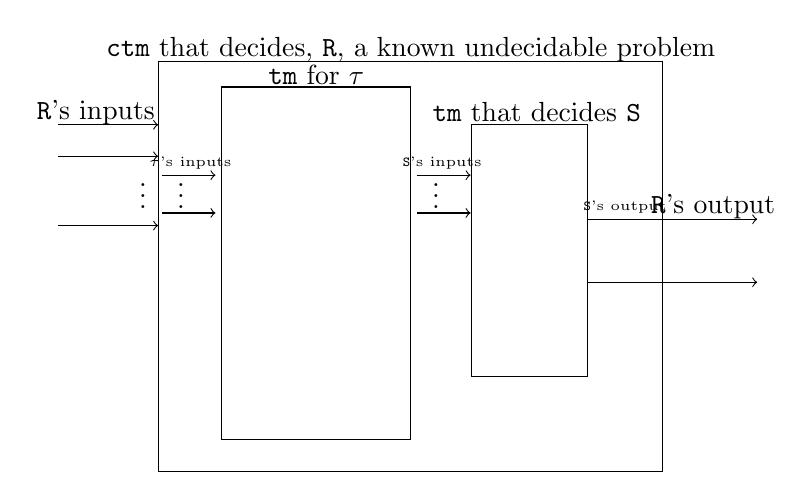
\begin{tikzpicture}[scale=0.8]
\draw (4,7.2) node {\ctm{} that decides, \texttt{R}, a known undecidable problem};
\draw (0,0.5) rectangle (8,7);
\draw (-1,6.2) node {\texttt{R}'s inputs};
\draw[->] (-1.6,6) -- (-0.01,6);
\draw[->] (-1.6,5.5) -- (-0.01,5.5);
\draw (-0.25,5) node {\vdotss};
\draw[->] (-1.6,4.4) -- (-0.01,4.4);
\draw (2.5,6.8) node {\tm{} for \texttt{$\tau$}};
\draw (1,1) rectangle (4,6.6);
\draw (0.5,5.4) node {\tiny{\texttt{$\tau$}'s inputs}};
%\draw[->] (0.05,6) -- (0.9,6);
\draw[->] (0.05,5.2) -- (0.9,5.2);
\draw (0.35,5) node {\vdotss};
\draw[->] (0.05,4.6) -- (0.9,4.6);

%\draw[->] (4.1,6) -- (4.95,6);
\draw[->] (4.1,5.2) -- (4.95,5.2);
\draw (4.4,5) node {\vdotss};
\draw[->] (4.1,4.6) -- (4.95,4.6);

\draw (6,6.2) node {\tm{} that decides \texttt{S}};
\draw (4.97,2) rectangle (6.8,6);
\draw (4.5,5.4) node {\tiny{\texttt{S}'s inputs}};

\draw[->] (6.8,4.5) -- (9.5,4.5);
\draw[->] (6.8,3.5) -- (9.5,3.5);
\draw (7.4,4.7) node {\tiny{\texttt{S}'s output}};

\draw (8.8,4.7) node {\texttt{R}'s output};
\end{tikzpicture}
\end{flushleft}

\end{itemize}
\end{tiny}
\end{frame}

\begin{frame}[fragile]
\frametitle{Church-Turing Thesis and Undecidability}
%\framesubtitle{HOMEWORK}
\begin{tiny}
\begin{itemize}
\item<1->
\begin{flushleft}
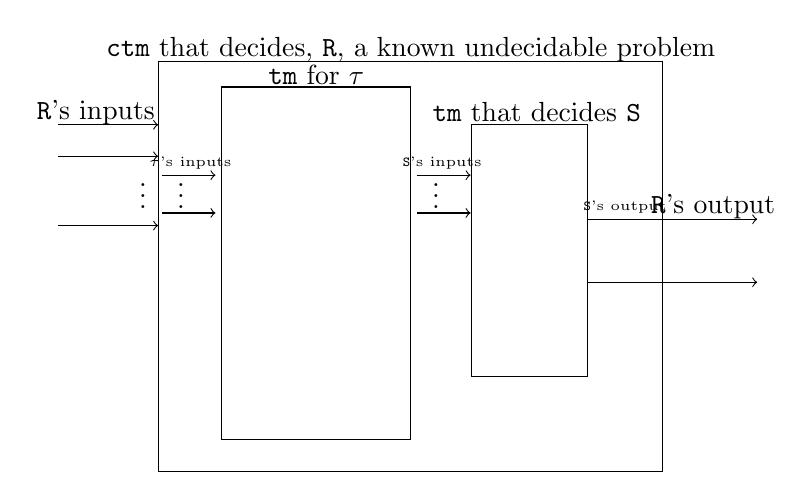
\begin{tikzpicture}[scale=0.8]
\draw (4,7.2) node {\ctm{} that decides, \texttt{R}, a known undecidable problem};
\draw (0,0.5) rectangle (8,7);
\draw (-1,6.2) node {\texttt{R}'s inputs};
\draw[->] (-1.6,6) -- (-0.01,6);
\draw[->] (-1.6,5.5) -- (-0.01,5.5);
\draw (-0.25,5) node {\vdotss};
\draw[->] (-1.6,4.4) -- (-0.01,4.4);
\draw (2.5,6.8) node {\tm{} for \texttt{$\tau$}};
\draw (1,1) rectangle (4,6.6);
\draw (0.5,5.4) node {\tiny{\texttt{$\tau$}'s inputs}};
%\draw[->] (0.05,6) -- (0.9,6);
\draw[->] (0.05,5.2) -- (0.9,5.2);
\draw (0.35,5) node {\vdotss};
\draw[->] (0.05,4.6) -- (0.9,4.6);

%\draw[->] (4.1,6) -- (4.95,6);
\draw[->] (4.1,5.2) -- (4.95,5.2);
\draw (4.4,5) node {\vdotss};
\draw[->] (4.1,4.6) -- (4.95,4.6);

\draw (6,6.2) node {\tm{} that decides \texttt{S}};
\draw (4.97,2) rectangle (6.8,6);
\draw (4.5,5.4) node {\tiny{\texttt{S}'s inputs}};

\draw[->] (6.8,4.5) -- (9.5,4.5);
\draw[->] (6.8,3.5) -- (9.5,3.5);
\draw (7.4,4.7) node {\tiny{\texttt{S}'s output}};

\draw (8.8,4.7) node {\texttt{R}'s output};
\end{tikzpicture}
\end{flushleft}

\item<1-> More formally, let \texttt{R} and \texttt{S} be two problems. A reduction from \texttt{R} to \texttt{S} is a transformation function, \texttt{$\tau$}, such that \texttt{x$\in$R $\Leftrightarrow$ $\tau$(x)$\in$S} and \texttt{x$\notin$R $\Leftrightarrow$ $\tau$(x)$\notin$S}
    
\item<2-> You may think of \texttt{$\tau$} as a function that is computable by a \tm{} that transforms a subset of inputs for \texttt{R} to inputs for \texttt{S} in such a manner that the answer returned by \texttt{S} means that we know the answer that \texttt{R} ought to return

\end{itemize}
\end{tiny}
\end{frame}

\begin{frame}[fragile]
\frametitle{Church-Turing Thesis and Undecidability}
%\framesubtitle{HOMEWORK}
\begin{scriptsize}
\begin{itemize}
\item<1->
\begin{theorem}
R is undecidable $\wedge \exists$ $\tau$ = a reduction function from R to S $\Rightarrow$ S is undecidable.
\end{theorem}

\item<2->
\begin{proof}
\mbox{}\\

\noindent Assume M$_{\texttt{S}}$ decides S and T computes $\tau$.\\

\noindent The \ctm{} T M$_{\texttt{S}}$ decides R. This is a contradiction. Therefore, S is undecidable.

\end{proof}

\item<3-> Alan Turing penned one of the great intellectual achievements of the 20$^{\texttt{th}}$ when in 1936 he proved that the halting problem was undecidable
    
\item<3-> It paved the way to prove that other problems are undecidable using reduction proofs
    
\item<3-> We shall explore undecidable problems about Turing machines

\end{itemize}
\end{scriptsize}
\end{frame}

\begin{frame}[fragile]
\frametitle{Church-Turing Thesis and Undecidability}
%\framesubtitle{HOMEWORK}
\begin{tiny}
\begin{itemize}
\item<1->
\begin{theorem}
Given a \tm{}, M, determining if M halts on \texttt{EMP} is undecidable.
\end{theorem}

\item<2->
\begin{proof}
\mbox{}\\

\noindent Assume \texttt{S} decides if M halts on \texttt{EMP}. That is, S decides the following language:
\begin{alltt}
     L = \{N | N is a tm{} or \ctm{} that halts on EMP\}
\end{alltt}
We shall use \texttt{S} to build a \ctm{}, \texttt{R}, that decides the halting problem.\\

\noindent The inputs for \texttt{R} are M and a word w. The reduction machine for \texttt{$\tau$} builds a \tm{}, \texttt{M}\quot{}, that operates as follows:
\begin{alltt}
 1. \texttt{M}\quot{}'s starting configuration is: (S 1 \qquot(,LM ,BLANK))
 2. \texttt{M}\quot{} writes w on the tape
 3. Moves the head to the first blank to the left (i.e., the
    first blank on the tape)
 4. Simulates M
\end{alltt}
Stated using the graphical \ctm{} notation, for w = a$_1$a$_2$\dotss{}$a_n$ \texttt{M}\quot{} is:
\begin{alltt}
     R a\(\sb{1}\) R a\(\sb{2}\)\dotss{}R a\(\sb{n}\) FBL M
\end{alltt}

\noindent \texttt{M}\quot{} is given as input to \texttt{S}. If \texttt{S} accepts then M halts on w and the \texttt{R}'s output is accept. Otherwise, if \texttt{S} rejects then M does not halt on w and the \texttt{R}'s output is reject. Given that the halting problem is undecidable, we have a contradiction and, therefore, \texttt{S} cannot exist.
\end{proof}

\end{itemize}
\end{tiny}
\end{frame}

\begin{frame}[fragile]
\frametitle{Church-Turing Thesis and Undecidability}
%\framesubtitle{HOMEWORK}
\begin{tiny}
\begin{itemize}
\item<1-> 
\begin{theorem}
Given a \tm{}, M, determining if their exists a word for which \texttt{M} halts is undecidable.
\end{theorem}

\item<2->
\begin{proof}
\mbox{}\\

\noindent Assume \texttt{S} decides if their exist any word for which a given \tm{} halts. That is, S decides the following language:
\begin{alltt}
     L = \{N | N is a tm{} or \ctm{} such that their exists a word
              for which \texttt{N} halts\}
\end{alltt}
We shall use \texttt{S} to build a \ctm{}, \texttt{R}, that decides if M halts on \texttt{EMP}. This language is proven undecidable in \Cref{tm-halts-emp}.\\

\noindent The input to \texttt{R} is, M, an arbitrary \tm{}. The reduction machine for \texttt{$\tau$} builds a \tm{}, \texttt{M}\quot{}, that operates as follows:
\begin{alltt}
 1. Erases its input
 2. Simulates M
\end{alltt}

\noindent \texttt{M}\quot{} is given as input to \texttt{S}. If \texttt{S} accepts this means that \texttt{M}\quot{} halts on some word if and only if it halts on all words. Therefore, M halts on \texttt{EMP}. Thus, \texttt{R} ought to accept. Otherwise, if \texttt{S} rejects this means that \texttt{M}\quot{} does not halt on any word if and only if it does not halt on all words. Therefore, M does not halt on \texttt{EMP}. Thus, \texttt{R} ought to reject. Given that determining if a \tm{} halts on \texttt{EMP} is undecidable, we have a contradiction and, therefore, \texttt{S} cannot exist.
\end{proof}

\end{itemize}
\end{tiny}
\end{frame}

\begin{frame}[fragile]
\frametitle{Church-Turing Thesis and Undecidability}
%\framesubtitle{HOMEWORK}
\begin{scriptsize}
\begin{itemize}
\item<1-> HOMEWORK: 6--8

\end{itemize}
\end{scriptsize}
\end{frame}

\begin{frame}[fragile]
\frametitle{Church-Turing Thesis and Undecidability}
%\framesubtitle{HOMEWORK}
\begin{scriptsize}
\begin{itemize}
\item<1-> 
\begin{theorem}
Given a \csg{}, G, determining if a word, w, is in the language generated by G is undecidable.
\end{theorem}

\item<2->
\begin{proof}
\mbox{}\\

\noindent Assume \texttt{S} decides if w$\in$L(G). That is, S decides the following language of doubles:
\begin{alltt}
     L = \{(G w) | G is a \csg{} and w\(\in\)L(G)\}
\end{alltt}
We shall use \texttt{S} to build a \ctm{}, \texttt{R}, that decides the halting problem.\\

\noindent The input to \texttt{R} is, M, an arbitrary \tm{}, and, w, an arbitrary word. The reduction machine for \texttt{$\tau$} builds a \csg{}, \texttt{G}\quot{}, using M and the construction algorithm sketched in \Cref{equiv-csg-tm}. \texttt{L(G\quot{})} is the language semidecided by M.\\

\noindent \texttt{G}\quot{} and w are given as input to \texttt{S}. If \texttt{S} accepts then we know that \texttt{G}\quot{} generates w. This means M halts and accepts w. Therefore, \texttt{R} ought to accept. If \texttt{S} rejects then we know that \texttt{G}\quot{} does not generate w. This means M does not halt on w. Therefore, \texttt{R} ought to reject. Given that the halting problem is undecidable, we have a contradiction and, therefore, \texttt{S} cannot exist.
\end{proof}

\end{itemize}
\end{scriptsize}
\end{frame}

\begin{frame}[fragile]
\frametitle{Church-Turing Thesis and Undecidability}
%\framesubtitle{HOMEWORK}
\begin{scriptsize}
\begin{itemize}
\item<1-> 
\begin{theorem}
Given a \csg{}, G, determining if L(G)=$\varnothing$ is undecidable.
\end{theorem}

\item<2->
\begin{proof}
\mbox{}\\

\noindent Assume \texttt{S} decides if L(G)=$\varnothing$. That is, S decides the following language of doubles:
\begin{alltt}
     L = \{G | G is a \csg{} and L(G)=\(\varnothing\)\}
\end{alltt}
We shall use \texttt{S} to build a \ctm{}, \texttt{R}, that decides if there is any word for which a \tm{} halts. This \tm{} problem is proven undecidable in \Cref{m-lang-not-empty}.\\

\noindent The input to \texttt{R} is, M, an arbitrary \tm{}. The reduction machine for \texttt{$\tau$} builds a \csg{}, \texttt{G}\quot{}, for M using the construction algorithm sketched in \Cref{equiv-csg-tm}. \texttt{L(G)}\quot{} is the language semidecided by M.\\

\noindent \texttt{G}\quot{} is given as input to \texttt{S}. If \texttt{S} accepts then we know that \texttt{L(G)\quot{}}=\texttt{$\varnothing$}. This means L(M) is empty. Therefore, \texttt{R} ought to reject. If \texttt{S} rejects then we know that \texttt{L(G)\quot{}}$\neq$\texttt{$\varnothing$}. This means L(M) is not empty. Therefore, \texttt{R} ought to accept. Given that determining if there is any word for which a \tm{} halts is undecidable, we have a contradiction and, therefore, \texttt{S} cannot exist.
\end{proof}

\end{itemize}
\end{scriptsize}
\end{frame}

\begin{frame}[fragile]
\frametitle{Church-Turing Thesis and Undecidability}
%\framesubtitle{HOMEWORK}
\begin{scriptsize}
\begin{itemize}
\item<1-> HOMEWORK: 11--12

\end{itemize}
\end{scriptsize}
\end{frame}

\section{Complexity}

\begin{frame}[fragile]
\frametitle{Complexity}
%\framesubtitle{HOMEWORK}
\begin{scriptsize}
\begin{itemize}
\item<1-> One of the principal threads in this book is nondeterminism

\item<2-> Are deterministic and nondeterministic Turing machines are equivalent?

\end{itemize}
\end{scriptsize}
\end{frame}

\begin{frame}[fragile]
\frametitle{Complexity}
%\framesubtitle{HOMEWORK}
\begin{scriptsize}
\begin{itemize}
\item<1-> A nondeterministic \tm{} may be simulated by a deterministic \tm{}

\item<2-> We shall develop an algorithm for a deterministic \tm{} to systematically simulate all the possible steps that a nondeterministic \tm{} may take--even those that do not lead to the machine halting or accepting
    
\item<2-> Exhaustive search of all the possible transitions the nondeterministic \tm{} can perform

\end{itemize}
\end{scriptsize}
\end{frame}

\begin{frame}[fragile]
\frametitle{Complexity}
%\framesubtitle{HOMEWORK}
\begin{scriptsize}
\begin{itemize}
\item<1->
\begin{center}
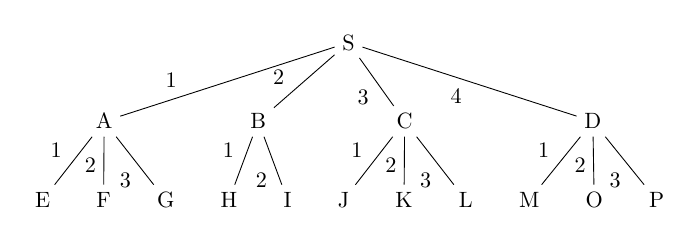
\begin{tikzpicture}[scale=0.8,level distance=1.25cm,sibling distance=.5cm,
   edge from parent path={(\tikzparentnode) -- (\tikzchildnode)}]
\Tree [.\node {S};
    \edge node[auto=right,pos=.7] {1};
    [.A
      \edge node[auto=right,pos=.6] {1};
      [.E ]
      \edge node[auto=right,pos=.6] {2};
      [.F ]
      \edge node[auto=right,pos=.6] {3};
      [.G ]
    ]
    \edge node[auto=right,pos=.7] {2};
    [.B
      \edge node[auto=right,pos=.6] {1};
      [.H ]
      \edge node[auto=right,pos=.6] {2};
      [.I ]
    ]
    \edge node[auto=right,pos=.5] {3};
    [.C
      \edge node[auto=right,pos=.6] {1};
      [.J ]
      \edge node[auto=right,pos=.6] {2};
      [.K ]
      \edge node[auto=right,pos=.6] {3};
      [.L ]
    ]
    \edge node[auto=right,pos=.5] {4};
    [.D
      \edge node[auto=right,pos=.6] {1};
      [.M ]
      \edge node[auto=right,pos=.6] {2};
      [.O ]
      \edge node[auto=right,pos=.6] {3};
      [.P ]
    ]
    ]
\end{tikzpicture}
\end{center}

\item<1-> Each node represents a configuration for \texttt{N}

\item<1-> The deterministic machine must simulate all paths

\item<1-> We need a systematic way to represent a computation

\item<1-> Number branches and encode branch chosen at each step

\item<1-> \texttt{(4 1)} = \texttt{S} \step{} \texttt{D} \step{} \texttt{M}

\end{itemize}
\end{scriptsize}
\end{frame}

\begin{frame}[fragile]
\frametitle{Complexity}
%\framesubtitle{HOMEWORK}
\begin{scriptsize}
\begin{itemize}
\item<1->
\begin{center}
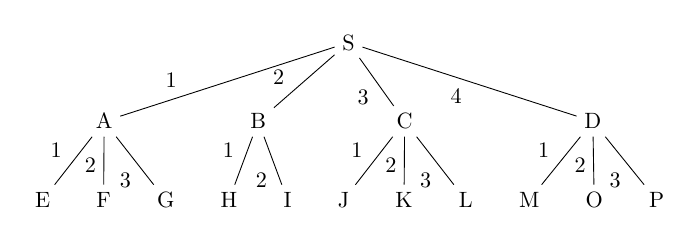
\begin{tikzpicture}[scale=0.8,level distance=1.25cm,sibling distance=.5cm,
   edge from parent path={(\tikzparentnode) -- (\tikzchildnode)}]
\Tree [.\node {S};
    \edge node[auto=right,pos=.7] {1};
    [.A
      \edge node[auto=right,pos=.6] {1};
      [.E ]
      \edge node[auto=right,pos=.6] {2};
      [.F ]
      \edge node[auto=right,pos=.6] {3};
      [.G ]
    ]
    \edge node[auto=right,pos=.7] {2};
    [.B
      \edge node[auto=right,pos=.6] {1};
      [.H ]
      \edge node[auto=right,pos=.6] {2};
      [.I ]
    ]
    \edge node[auto=right,pos=.5] {3};
    [.C
      \edge node[auto=right,pos=.6] {1};
      [.J ]
      \edge node[auto=right,pos=.6] {2};
      [.K ]
      \edge node[auto=right,pos=.6] {3};
      [.L ]
    ]
    \edge node[auto=right,pos=.5] {4};
    [.D
      \edge node[auto=right,pos=.6] {1};
      [.M ]
      \edge node[auto=right,pos=.6] {2};
      [.O ]
      \edge node[auto=right,pos=.6] {3};
      [.P ]
    ]
    ]
\end{tikzpicture}
\end{center}

\item<1-> The deterministic machine can perform a breadth-first search of the computation tree exploring shorter paths before longer paths
    
\item<2-> Key to making this process systematic is to define an increment function for a word (of encoded numbers) on the tape
    
\item<2-> The increment function may be described as follows:
\begin{enumerate}
  \item If the rightmost number is less than \texttt{r} add 1 to it.
  \item If the rightmost number is \texttt{r} make it 1 and propagate a 1 to the left.
  \item During left propagation if a number is less than \texttt{r} add 1 to it. If the number is \texttt{r} make it a 1 and propagate left. If the blank is read then make the blank a 1 and shift the number one space to the right.
\end{enumerate}

\end{itemize}
\end{scriptsize}
\end{frame}

\begin{frame}[fragile]
\frametitle{Complexity}
%\framesubtitle{HOMEWORK}
\begin{tiny}
\begin{itemize}
\item<1-> 
\begin{alltt}
     (1) represents the computation S \step{} A
     (2) represents the computation S \step{} B
     (3) represents the computation S \step{} C
     (4) represents the computation S \step{} D
\end{alltt}

\item<2-> At this point, the number equals \texttt{r} and the increment must propagate left:
\begin{alltt}
     (1 1) represents the computation S \step{} A \step{} E
     (1 2) represents the computation S \step{} A \step{} F
     (1 3) represents the computation S \step{} A \step{} G
     (1 4) represents a computation that does not exist
\end{alltt}

\item<3-> Once again, the number equals \texttt{r} and the increment must propagate left:
\begin{alltt}
     (2 1) represents the computation S \step{} B \step{} H
     (2 2) represents the computation S \step{} B \step{} I
     (2 3) represents a computation that does not exist
     (2 4) represents a computation that does not exist
\end{alltt}

\end{itemize}
\end{tiny}
\end{frame}

\begin{frame}[fragile]
\frametitle{Complexity}
%\framesubtitle{HOMEWORK}
\begin{scriptsize}
\begin{itemize}
\item<1-> We can now outline an algorithm for a \tm{} to systematically search a computation tree
    
\item<1-> It shall use an iterative deepening strategy

\item<1-> 3 main values (more values are needed in an actual implementation): the input word \texttt{w}, \texttt{N}'s current configuration \texttt{C}, and the encoded number, \texttt{I}, representing the current computation performed
    
\item<2-> The machine's operation is outlined as follows:
\begin{alltt}
     1. If N's starting state is a final state then halt.
     2. Start with N's starting configuration and I = (1).
     3. Perform the computation encoded by I if possible.
        If not possible ignore the rest of I and return C.
     4. Check the configuration returned by Step 3. If it is
        in one of N's halting  states then halt. Otherwise,
        increment I, restore N's starting configuration and
        go to step 3.
\end{alltt}

\end{itemize}
\end{scriptsize}
\end{frame}

\begin{frame}[fragile]
\frametitle{Complexity}
%\framesubtitle{HOMEWORK}
\begin{tiny}
\begin{itemize}
\item<1-> 
\begin{theorem}
A nondeterministic \tm{} semidecides L $\Rightarrow$ $\exists$ a deterministic \tm{} that semidecides L
\end{theorem}

\item<2->
\begin{proof} (Sketch)
\mbox{}\\

\noindent Assume N is a nondeterministic \tm{} that semidecides L.

\begin{itemize}
\item<3-> \tiny An \mttm{} with 5 main tapes shall simulate N. The purpose of each tape is described as follows:
\begin{alltt}
  Tape 0: Contains the input word, w, and is never mutated
  Tape 1: Used to simulate N by recording N's configuration
  Tape 2: Stores, I, the next computation number
  Tape 3: Stores N's rules
  Tape 4: Stores the rules applicable to the current
          configuration on Tape 1
\end{alltt}
More tapes may be needed to manage low-level details, but we shall not concern ourselves with these details at this time. Clearly, an \mttm{} may have as many tapes as needed.

\item<4-> \tiny The \mttm{} starts with the input word, w, on tape 0 and operates as follows:
\begin{alltt}
 1. Write the encoding for the computation number \quot{}(1) onto tape 3
 2. Write N's starting configuration on tape 2 using w on tape 1
 3. Read the rightmost unprocessed encoded element, k, in the computation 
    number on tape 3
 4. Extract the rules from tape 3 that may be used on the configuration on 
    tape 1 and copy them to tape 4
 5. Apply the k\(\sp{\textrm{th}}\) rule on tape 4 to configuration on tape 1 and mutate tape 1 
    to store this new configuration. If no such rule exists go to the next step.
 6. Check if tape 1 contains a halting configuration
    a. If so, halt
    b. Otherwise, increment the computation number on tape 3 and goto step 2
\end{alltt}
\end{itemize}
\end{proof}

\end{itemize}
\end{tiny}
\end{frame}

\begin{frame}[fragile]
\frametitle{Complexity}
%\framesubtitle{HOMEWORK}
\begin{scriptsize}
\begin{itemize}
\item<1-> HOMEWORK: 1

\end{itemize}
\end{scriptsize}
\end{frame}

\begin{frame}[fragile]
\frametitle{Complexity}
%\framesubtitle{HOMEWORK}
\begin{tiny}
\begin{itemize}
\item<1-> Is the solution to a solvable problem practical?

\item<2-> To explore whether or not solvable implies a practical solution, we shall discuss the traveling salesman problem (\texttt{TSP})

\item<2-> Given \texttt{k} cities and the distances between each pair of them, find the shortest itinerary that returns to its starting point and visits each other city exactly once along the way
    
\item<3-> This problem is clearly solvable:
\begin{alltt}
     1. List all possible itineraries that satisfy the
        constraint of visiting each city once
     2. Return the itinerary with the shortest distance
\end{alltt}


\item<4-> How many times must a sum be computed?
\begin{alltt}
                   City: A ___ ___ ___ \dotss{}  ___  ___ A
     Itinerary position: 0  1   2   3      k-2  k-1 k
\end{alltt}


\item<5-> The number of different itineraries is equal to \texttt{(k - 1)!}

\item<6-> What if our hypothetical salesman must travel to 50 cities?

\item<7-> 49! = 608281864034267560872252163321295376887552831379210240000000000

\item<7-> If 10 billion itineraries could be processed per second, faster than any computer in the 
          foreseeable future, then it would take about 1928849137602319764308257747721002590333437440 years to find the shortest itinerary

\item<8-> Grows faster than \texttt{2$^{\texttt{k}}$}

\item<8-> The growth function is an exponential function and renders the solution impractical

\end{itemize}
\end{tiny}
\end{frame}

\begin{frame}[fragile]
\frametitle{Complexity}
%\framesubtitle{HOMEWORK}
\begin{scriptsize}
\begin{itemize}
\item<1-> We need a way to characterize solutions that are practical (i.e., polynomial growth) 
    
\item<1-> This eliminates deterministic \tm{}s that simulate nondeterministic \tm{}s
    
\item<2-> We define the set of Turing machines (i.e., algorithms) that are practical as:
\begin{alltt}
  \p{} = \{M | M is a deterministic Turing machine that decides
           a language or computes a function in a number of
           steps proportional to n\(\sp{k}\)\}
\end{alltt}

\item<2-> We say that any problem solvable by a \tm$\in$\p{} is \emph{tractable}.

\item<3-> Not every practical algorithm (i.e., in \p{}) means it is suitable for use in every day computing
    
\item<3-> Consider a deterministic \tm{} whose number of steps is proportional to \texttt{n$^{\texttt{10}}$}
    
\item<3-> For a modest input size of 100, the number of operations is proportional to \texttt{10$^{\texttt{100}}$}
    
\item<3-> It is difficult to see how such an algorithm can be practical for other than the smallest instances of the problem solved
    
\item<3-> Thankfully, most algorithms of interest to industry programmers are solved in a number of steps proportional to \texttt{n$^{\texttt{3}}$} or less.

\end{itemize}
\end{scriptsize}
\end{frame}

\begin{frame}[fragile]
\frametitle{Complexity}
%\framesubtitle{HOMEWORK}
\begin{scriptsize}
\begin{itemize}
\item<1-> We can prove properties of \p{} just like we proved properties for other classes of languages
    
\item<2-> For instance, \p{} is closed under complement.

\item<3->
\begin{theorem}
\p{} is closed under complement.
\end{theorem}

\item<4->
\begin{proof}
\mbox{ }\\

\noindent Let M = (make-tm K \sig{} R S \quot{}(Y N) \quot{}Y) be deterministic and decide a language L in polynomial time. This means M$\in$\p{}. The interpretation of the final states is as you may expect: Y is for accept and N is for reject.\\

\noindent From M, we can build a deterministic Turing machine, \={M}, to decide L's complement in polynomial time. Every word accepted by M ought to be rejected by \={M} and every word rejected by M ought to be accepted by \={M}. To achieve this, \={M} is the same as M except that the roles of Y and N are swapped. In this manner, \={M} only accepts if M would have rejected and viceversa.
\end{proof}

\end{itemize}
\end{scriptsize}
\end{frame}

\begin{frame}[fragile]
\frametitle{Complexity}
%\framesubtitle{HOMEWORK}
\begin{scriptsize}
\begin{itemize}
\item<1-> 
\begin{alltt}
;; tm-language-recognizer \arrow{} tm-language-recognizer
;; Purpose: Build a deterministic tm-language-recognizer for
;;          the complement of the language decided by the 
;;          given deterministic tm-language-recognizer
;; Assumption: Given tm's final states are Y and N
;;             and Y is the accepting state
(define (dtm4L->dtm4notL M)
  (make-tm (sm-states M)
           (sm-sigma M)
           (sm-rules M)
           (sm-start M)
           (sm-finals M)
           \quot{}N))
\end{alltt}
\end{itemize}
\end{scriptsize}
\end{frame}

\begin{frame}[fragile]
\frametitle{Complexity}
%\framesubtitle{HOMEWORK}
\begin{tiny}
\begin{itemize}
\item<1-> A classical problem discussed to illustrate if a problem is or is not in \p{} is the Boolean satisfiability problem
    
\item<1-> The Boolean satisfiability problem takes as input a Boolean formula in conjunctive normal form and determines if the formula is satisfiable 

\item<2-> Consider:
\begin{alltt}
     (and (or x y) (not x) (or y z))
\end{alltt}

\item<3-> This formula is satisfiable. Make \texttt{x = \#f}:
\begin{alltt}
     (and (or \#f (not y)) \#t (y \(\vee\) z))
     (and (not y) (or y z)
\end{alltt}

\item<4-> Make \texttt{y = \#f}:
\begin{alltt}
     (and \#t (or \#f z)
     z
\end{alltt}

\item<5-> Making \texttt{z = \#t} establishes the formula is satisfiable

\item<6->  In contrast, the following formula is not satisfiable:
\begin{alltt}
   (and (or x y z)
        (or (not x) (not y) (not z))
        (or x (not y))
        (or y (not z))
        (or (not x) z))
\end{alltt}

\item<6-> \texttt{(or x y z)}, is satisfied if any variable is true

\item<6-> \texttt{(or (not x) (not y) (not z))} is satisfied if any variable is false

\item<6-> At least one variable must be true and at least one variable must be false
    
\item<7-> The remaining conjunction:
\begin{alltt}
     (and (or x (not y)) (or y (not z)) (or (not x) z))
\end{alltt}

\item<7-> Only satisfiable if the value of all three variables is the same

\end{itemize}
\end{tiny}
\end{frame}

\begin{frame}[fragile]
\frametitle{Complexity}
%\framesubtitle{HOMEWORK}
\begin{scriptsize}
\begin{itemize}
\item<1-> We shall now explore how to solve a simplified version of the Boolean satisfiability problem called the 2-satisfiability problem
    
\item<1-> In this simplified version every clause of a formula in disjunctive normal form is either a singleton or a 2-disjunction
    
\item<2-> The solution presented shall draw upon our knowledge of grammars to represent input formulae given by the user
    
\item<2-> In addition, the grammar for input formulae is used to develop a formula parser
    
\item<2-> As you may have learned in a Programming Languages course, parsers produce parse trees that eliminate the need for superfluous information like parentheses and keywords (e.g., \texttt{not} and \texttt{or})

\end{itemize}
\end{scriptsize}
\end{frame}

\begin{frame}[fragile]
\frametitle{Complexity}
%\framesubtitle{HOMEWORK}
\begin{tiny}
\begin{itemize}
\item<1-> Context-Free Grammar for the 2-Satisfiability Problem Formulae
\begin{alltt}
          iformula \arrow{} \quot{}(and iclauses)

          iclauses \arrow{} ()
                   \arrow{} (cons iclause iclauses)

           iclause \arrow{} isingleton
                   \arrow{} i2disjunction

        isingleton \arrow{} symbol
                   \arrow{} (not symbol)

     i2disjunction \arrow (or isingleton isingleton)
\end{alltt}

\item<2-> Representation for the abstract 

\item<2-> We define formula as follows:
\begin{alltt}
     ;; A formula \arrow{} \elist
     ;;           \arrow{} (cons clause formula)
\end{alltt}

\item<3-> A clause is defined as follows:
\begin{alltt}
     ;; clause \arrow{} singleton
     ;;        \arrow{} 2disjunction
\end{alltt}

\item<4-> A singleton is defined as follows:
\begin{alltt}
     ;; singleton \arrow{} (var symbol)
     ;;           \arrow{} (notvar symbol)

     (struct var (symb) #:transparent)
     (struct notvar (symb) #:transparent)
\end{alltt}

\item<5-> A disjunction is represented as follows:
\begin{alltt}
     ;; disjunction \arrow{} (2disjunction singleton singleton)

     (struct 2disjunction (s1 s2) #:transparent)
\end{alltt}

\end{itemize}
\end{tiny}
\end{frame}

\begin{frame}[fragile]
\frametitle{Complexity}
%\framesubtitle{HOMEWORK}
\begin{tiny}
\begin{itemize}
\item<1-> The parser
\begin{alltt}
     ;; iformula \arrow{} formula
     ;; Purpose: Parse the given iformula
     (define (parse-iformula an-iformula)
\end{alltt}

\item<2->
\begin{alltt}
       ;; icl \arrow{} clause
       ;; Purpose: Parse the given icl
       (define (parse-iclause an-icl)
\end{alltt}

\item<4->
\begin{alltt}
         ;; isingleton \arrow{} singleton
         ;; Purpose: Parse the given isingleton
         (define (parse-isingleton an-is)
           (if (symbol? an-is)
               (var an-is)
               (notvar (second an-is))))
\end{alltt}

\item<5->
\begin{alltt}
         ;; idisjunction \arrow{} disjunction
         ;; Parse: Parse the given idisjunction
         (define (parse-i2disjunction an-id)
           (2disjunction (parse-isingleton (first an-id))
                         (parse-isingleton (second an-id))))
\end{alltt}

\item<3->
\begin{alltt}
         ;; iclause \arrow{} Boolean
         ;; Purpose: Determine if the given iclause is an isingleton
         (define (isingleton? an-icl)
           (or (symbol? an-icl)
               (eq? (first an-icl) \quot{}not)))
\end{alltt}

\item<2->
\begin{alltt}
        (if (isingleton? an-icl)
            (parse-isingleton an-icl)
            (parse-i2disjunction (rest an-icl))))
\end{alltt}

\item<1->
\begin{alltt}
      (map parse-iclause (rest an-iformula)))
\end{alltt}

\end{itemize}
\end{tiny}
\end{frame}

\begin{frame}[fragile]
\frametitle{Complexity}
%\framesubtitle{HOMEWORK}
\begin{tiny}
\begin{itemize}
\item<1-> The 2-satisfiability solver searches for a set of assignments to satisfy a given \texttt{formula}
    
\item<1-> Returns \texttt{\quot{}accept} if variables may be assigned values that satisfy the formula. Otherwise, \texttt{\quot{}reject} is returned.

\item<2-> An accumulator to store the current variable assignments in a list is used
    
\item<2-> The accumulator invariant is that the accumulator contains the variable bindings made so far to satisfy the formula
    
\item<2-> The function first checks if any variable assignment is possible

\item<2-> If the given formula is empty then all needed variable assignments have been made and the accumulator is returned
     
\item<2-> If the formula has no solution then the empty list is returned

\item<2-> A formula has no solution when a variable and its complement are both clauses in the formula

\item<3-> If the formula contains one or more singletons the function assigns a value to a single variable, simplifies the formula based on the assignment made, and recursively searches for assignments using the simplified formula
    
\item<4-> If the formula does not contains any singleton clauses then it must only contain disjunctions
    
\item<4-> In this case, a backtracking strategy is used

\item<4-> The first clause's first singleton is assigned a value, the formula is simplified based on the assignment, and the simplified formula is solved
     
\item<4-> If this search is successful then the found list of bindings is returned 
    
\item<4-> Otherwise, the first clause's first singleton is assigned the complement of its first assignment, the formula is simplified based on this new assignment, and the simplified formula is solved
    
\item<4-> The result of this second search for assignments is returned.

\end{itemize}
\end{tiny}
\end{frame}

\begin{frame}[fragile]
\frametitle{Complexity}
%\framesubtitle{HOMEWORK}
\begin{scriptsize}
\begin{itemize}
\item<1-> The solver must distinguish between four properties the given formula may have:
\begin{enumerate}
\item The formula is empty.
\item The formula has no solution because it contains both a variable and its complement as clauses.
\item The formula contains a singleton.
\item The formula only contains disjunctions.
\end{enumerate}

\end{itemize}
\end{scriptsize}
\end{frame}

\begin{frame}[fragile]
\frametitle{Complexity}
%\framesubtitle{HOMEWORK}
\begin{tiny}
\begin{itemize}
\item<1-> The 2-Satisfiability Solver
\begin{alltt}
;; formula \arrow{} Boolean     Purpose: Determine if given formula is satisfiable
(define (2-satisfiability a-formula)
  \dotss{}
\end{alltt}

\item<2->
\begin{alltt}
  (define (solve a-formula acc)
\end{alltt}

\item<3->
\begin{alltt}
    (cond [(empty? a-formula) acc]
\end{alltt}

\item<4->
\begin{alltt}
          [(has-no-solution? (filter (\lamb{} (c) (not (2disjunction? c))) a-formula))
           \elist{}]
\end{alltt}

\item<5->
\begin{alltt}
          [(ormap (\lamb{} (c) (or (var? c) (notvar? c))) a-formula)
           (let [(form-vars (filter var? a-formula))
                 (form-notvars (filter notvar? a-formula))]
             (solve (remove-duplicates
                     (simplify-formula a-formula
                                       (if (null? form-notvars)
                                           (first form-vars)
                                           (first form-notvars))))
                    (if (null? form-notvars)
                        (cons (list (var-symb (first form-vars)) \#t) acc)
                        (cons (list (notvar-symb (first form-notvars)) \#f) acc))))]
\end{alltt}

\item<6->
\begin{alltt}
          [else ;; a-formula only has 2disjunctions
           (let* [(fsingleton (2disjunction-s1 (first a-formula)))
                  (fvar (if (var? fsingleton)
                            (var-symb fsingleton)
                            (notvar-symb fsingleton)))
                  (not-fsingleton (complement-singleton fsingleton))
                  (sol1 (solve (simplify-formula a-formula fsingleton)
                               (cons (list fvar (var? fsingleton)) acc)))]
             (if (not (null? sol1))
                 sol1
                 (solve (simplify-formula a-formula not-fsingleton)
                        (cons (list fvar (notvar? fsingleton)) acc))))]))
\end{alltt}

\item<1->
\begin{alltt}
  (if (not (null? (solve a-formula \elist{}))) \quot{}accept \quot{}reject))
\end{alltt}

\end{itemize}
\end{tiny}
\end{frame}

\begin{frame}[fragile]
\frametitle{Complexity}
%\framesubtitle{HOMEWORK}
\begin{scriptsize}
\begin{itemize}
\item<1-> Is the 2-Satisfiability Problem is in \p{}?

\item<2-> Number of variables in the given formula \texttt{n}

\item<3-> \texttt{complement-singleton} performs a constant number of operations

\item<4-> For \texttt{has-no-solution?}  the number of operations performed is proportional to \texttt{n$^{\texttt{2}}$}
    
\item<5-> For \texttt{simplify} the number of operations is proportional to \texttt{n}
    
\item<6-> For \texttt{simplify-formula}, that uses \texttt{simplify}, the number of operations performed is proportional to \texttt{n$^{\texttt{2}}$}
    
\item<7-> For \texttt{solve}, in the worst case 2\texttt{n} recursive calls are made and for each \texttt{n$^{\texttt{2}}$} operations are done.
    
\item<8-> In the worst case, the total number of operations is proportional to \texttt{n$^{\texttt{3}}$}
    
\item<8-> The 2-satisfiability problem is in \p{}. 

\end{itemize}
\end{scriptsize}
\end{frame}

\begin{frame}[fragile]
\frametitle{Complexity}
%\framesubtitle{HOMEWORK}
\begin{scriptsize}
\begin{itemize}
\item<1-> A primary goal of complexity theory is to discover mathematical approaches to establish that solutions to practical problems are not in \texttt{P}
    
\item<1-> One such problem we have discussed that appears not to be in \texttt{P} is the traveling salesman problem
     
\item<1-> We use the word \emph{appears}, because the best known algorithm implemented as a deterministic Turing machine takes an exponential number of steps to find the solution
     
\item<1-> A nondeterministic Turing machine finds the solution in a polynomial number of steps
    
\item<2-> Separating nondeterminism and determinism in terms of polynomial running time is one of the biggest and most profound problems in Computer Science
    
\item<2-> It is an open research question and remains unanswered

\item<3-> To explore problems not in \p{}, it helps to formally define what it means that a computation by a nondeterministic Turing machine is bounded by a polynomial number of steps
    
\item<3-> A nondeterministic Turing machine, \texttt{M}, is bounded by a polynomial, \texttt{p(n)}, if there is no (possible) computation that takes more than \texttt{p(n)} steps
    
\item<4-> We define the nondeterministic polynomial class of languages, \texttt{NP}, as those languages decided by a polynomially bounded nondeterministic Turing machine

\end{itemize}
\end{scriptsize}
\end{frame}

\begin{frame}[fragile]
\frametitle{Complexity}
%\framesubtitle{HOMEWORK}
\begin{scriptsize}
\begin{itemize}
\item<1->Computation tree for a nondeterministic Turing machine
\begin{center}
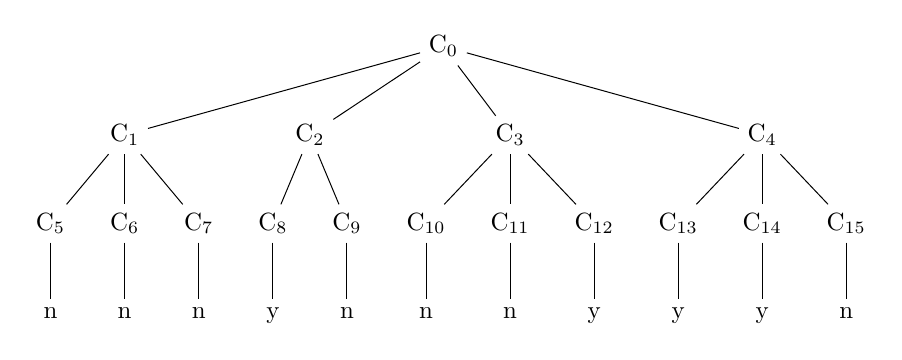
\begin{tikzpicture}[scale=0.9,level distance=1.25cm,sibling distance=.4cm,
   edge from parent path={(\tikzparentnode) -- (\tikzchildnode)}]
\Tree [.\node {C$_0$};
    \edge node[auto=right,pos=.7] {};
    [.C$_1$
      \edge node[auto=right,pos=.6] {};
      [.C$_5$
       \edge node[auto=right,pos=.6] {};
       [.n ]
      ]
      \edge node[auto=right,pos=.6] {};
      [.C$_6$
       \edge node[auto=right,pos=.6] {};
       [.n ]
      ]
      \edge node[auto=right,pos=.6] {};
      [.C$_7$
       \edge node[auto=right,pos=.6] {};
       [.n ]
      ]
    ]
    \edge node[auto=right,pos=.7] {};
    [.C$_2$
      \edge node[auto=right,pos=.6] {};
      [.C$_8$
       \edge node[auto=right,pos=.6] {};
       [.y ]
      ]
      \edge node[auto=right,pos=.6] {};
      [.C$_9$
       \edge node[auto=right,pos=.6] {};
       [.n ]
      ]
    ]
    \edge node[auto=right,pos=.5] {};
    [.C$_3$
      \edge node[auto=right,pos=.6] {};
      [.C$_{10}$
       \edge node[auto=right,pos=.6] {};
       [.n ]
      ]
      \edge node[auto=right,pos=.6] {};
      [.C$_{11}$
       \edge node[auto=right,pos=.6] {};
       [.n ]
      ]
      \edge node[auto=right,pos=.6] {};
      [.C$_{12}$
       \edge node[auto=right,pos=.6] {};
       [.y ]
      ]
    ]
    \edge node[auto=right,pos=.5] {};
    [.C$_4$
      \edge node[auto=right,pos=.6] {};
      [.C$_{13}$
       \edge node[auto=right,pos=.6] {};
       [.y ]
      ]
      \edge node[auto=right,pos=.6] {};
      [.C$_{14}$
       \edge node[auto=right,pos=.6] {};
       [.y ]
      ]
      \edge node[auto=right,pos=.6] {};
      [.C$_{15}$
       \edge node[auto=right,pos=.6] {};
       [.n ]
      ]
    ]
    ]
\end{tikzpicture}
\end{center}

\item<1-> Recall that a deterministic Turing machine may simulate a nondeterministic Turing machine by performing a breadth-first traversal 
    
\item<1-> Clear why nondeterminism in Turing machines is so powerful

\item<1-> Only the configurations on a single path to accept need to be visited 

\end{itemize}
\end{scriptsize}
\end{frame}

\begin{frame}[fragile]
\frametitle{Complexity}
%\framesubtitle{HOMEWORK}
\begin{tiny}
\begin{itemize}
\item<1-> Most computer scientists today believe that the Boolean satisfiability problem is not in \p{}
    
\item<1-> We shall demonstrate that it is \np{}

\item<1-> Specifically, we shall describe a nondeterministic 2-tape Turing machine that decides the Boolean satisfiability problem

\item<2-> Represent true as \texttt{T} and false as \texttt{F}

\item<2-> \texttt{n} denotes the number of (distinct) variables and \texttt{m} denotes the number of clauses

\item<3-> The machine operates in three stages:
\begin{enumerate}
\item \tiny For every distinct variable in the formula on tape 1 write an \texttt{x} on tape 2.
\item \tiny Nondeterministically, write an assignment on tape 2. Each \texttt{x} on tape 2 is nondeterministically substituted with a \texttt{T} or an \texttt{F}.
\item \tiny Check that each clause in the formula on tape 1 contains a singleton that is true given the assignment on tape 2. If this is the case, the formula is satisfiable and the machine accepts. Otherwise, it rejects.
\end{enumerate}

\item<4-> Stage 1 is accomplished deterministically in a polynomial number of steps: \texttt{n$^{\texttt{2}}$}

\item<5-> Stage 2 is accomplished nondeterministically in \texttt{n} steps by traversing the \texttt{x}s on tape 2
    
\item<6-> Stage 3 is done deterministically by processing the \texttt{m} clauses

\item<6->  For each clause, its singletons are traversed to determine if any evaluates to true
    
\item<6-> If all clauses are processed, then the machine accepts

\item<7-> To process a clause, the number of singletons is bounded by \texttt{2n} 
    
\item<7-> For each plug-in its value

\item<7-> If it evaluates to true, then the machine moves to the next clause

\item<7-> If it evaluates to false, then it moves to the next singleton in the clause
    
\item<7-> If none of the singletons evaluate to true then the machine moves to reject
    
\item<7-> The number of steps for stage 3 is proportional to \texttt{m*2n}

\item<8-> The toal number of operations is proportional to  \texttt{n$^{\texttt{2}}$} + \texttt{n} + \texttt{(max n m)$^{\texttt{2}}$} 
    
\item<8-> The Boolean satisfiability problem is in \np{}

\end{itemize}
\end{tiny}
\end{frame}

\begin{frame}[fragile]
\frametitle{Complexity}
%\framesubtitle{HOMEWORK}
\begin{scriptsize}
\begin{itemize}
\item<1-> Demonstrating that a problem is in \np{} requires solving a problem using a nondeterministic Turing machine that is bounded by a polynomial number of steps
    
\item<2-> An interesting question we may ask ourselves, is \np{} closed under complement? 
    
\item<3-> The answer to this question is currently unknown

\item<3-> Many properties of \np{} remain elusive to establish and this is an area of active research

\item<4-> One property that is immediately obvious, however, is that \p{}$\subseteq$\np{}
    
\item<4-> This follows by observing that a deterministic Turing machine is a nondeterministic Turing machine whose transition relation is a function
    
\item<5-> This observation suggests another question: Is \p{} = \np{}? 

\item<6-> This question remains unanswered and is one of the biggest unsolved problems in Computer Science
    
\end{itemize}
\end{scriptsize}
\end{frame}

\begin{frame}[fragile]
\frametitle{Complexity}
%\framesubtitle{HOMEWORK}
\begin{scriptsize}
\begin{itemize}
\item<1-> HOMEWORK: 6

\end{itemize}
\end{scriptsize}
\end{frame}

\section{Farewell and where to go from here?}

\begin{frame}[fragile]
\frametitle{Farewell and where to go from here?}
%\framesubtitle{HOMEWORK}
\begin{scriptsize}
\begin{itemize}
\item<1-> Congratulations! You have completed your first steps into the thought-provoking world of Theoretical Computer Science
     
\item<1-> You have learned about different models of computation: their powers and their limitations
    
\item<1-> You have also learned about nondeterminism and the role it plays in Computer Science and in programming
    
\item<1-> The models you have studied have varied applications across computer science. Explore them!
    
\item<2-> Most importantly, you now understand how machines compute functions, how decidability problems may be solved, and the meaning of the word \emph{algorithm}
    
\item<2-> Understanding what an algorithm is has naturally led to thinking about what can and can not be computed and what it means for a solution to be practical
    
\item<2-> You have become a better programmer and you have begun to explore some of humanity's limitations

\end{itemize}
\end{scriptsize}
\end{frame}

\begin{frame}[fragile]
\frametitle{Farewell and where to go from here?}
%\framesubtitle{HOMEWORK}
\begin{scriptsize}
\begin{itemize}
\item<1-> Believe it or not, you have only touched the tip of the iceberg when it comes to formal languages, automata theory, and complexity theory
    

\item<2-> Is it possible for a \cfg{} to always derive a word or state that the word is not in the language? 
    
\item<3-> It turns out that the answer to this question is almost always yes for ``long'' words by transforming to Chomsky normal form or Greibach normal form
    
\item<4-> Equally intriguing, there are many examples of undecidable problems you can explore
    
\item<4-> Consider a set of dominos such that each domino has two words on the same face (e.g., one of the top and one on the bottom)
    
\item<4-> Can dominos be placed in a row (repetitions allowed) such that the appending of top strings is the same as the appending of the bottom strings? 
    
\item<5-> This fun puzzle is known as the Post correspondence problem and it is an unsolvable problem

\end{itemize}
\end{scriptsize}
\end{frame}

\begin{frame}[fragile]
\frametitle{Farewell and where to go from here?}
%\framesubtitle{HOMEWORK}
\begin{scriptsize}
\begin{itemize}
\item<1-> There are also a myriad of topics you may explore that are not directly suggested by the topics covered in this textbook
    
\item<2-> Have you ever heard of quantum finite automata? 

\item<3-> Automata theory has applications in quantum computing

\item<4-> Automata theory also has applications in program verification

\item<4-> There is a special kind of invariant known as a \emph{preserved invariant}
    
\item<4-> A preserved invariant is one such that if it holds for some state \texttt{Q} then it also holds for any state reachable from \texttt{Q}
     
\item<4-> This fascinating type of invariant may be used to prove that software is correct
    
\item<5-> State-based machines also have alluring applications in artificial intelligence
    
\item<5-> \emph{neural} \tm{}s are used to model artificial neural networks that exhibit temporal dynamic behavior

\end{itemize}
\end{scriptsize}
\end{frame}

\begin{frame}[fragile]
\frametitle{Farewell and where to go from here?}
%\framesubtitle{HOMEWORK}
\begin{scriptsize}
\begin{itemize}
\item<1-> You are now well-equipped to explore formal languages and automata theory applications in many fields of Computer Science as well as to deepen your understanding of Computer Science's theoretical underpinnings
    
\item<1-> You may do so by either by taking more advanced courses or by personal inquiry
    
\item<1-> Regardless of your approach, you bring with you actual programming experience with state-based machines, grammars, and regular expressions
    
\item<1-> Mind what you have learned and apply it in your future intellectual endeavors
    
\item<2-> Above all, enjoy the challenges that come with process of discovery and the rigor required to prove your designs correct!
    
\item<2-> Adi\'{o}s!
\tikzsymbolsset{symbol-scale={ dCooley= 5 }}
\begin{center}
\dCooley
\end{center}

\end{itemize}
\end{scriptsize}
\end{frame}



\end{document} 